% This template mostly comes from Yiyang JIANG


\documentclass{beamer}
\usepackage{ctex, hyperref}
\usepackage[T1]{fontenc}

% other packages
\usepackage{latexsym,amsmath,xcolor,multicol,booktabs,calligra}
\usepackage{graphicx,pstricks,listings,stackengine}

\author{\href{}{Franciele Alba da Silva\\ 
Ruben Manso}}
\institute{\href{}{University of Applied Forest Sciences Rottenburg\\ Forest Research-UK }}
\title{Assessment of the Uncertainty from Different Sources in Forest Inventories}
\subtitle{}
\date{}
\usepackage{JYY_Beamer}

% defs
\def\cmd#1{\texttt{\color{green}\footnotesize $\backslash$#1}}
\def\env#1{\texttt{\color{blue}\footnotesize #1}}
\definecolor{deepblue}{rgb}{0,0,0.5}
\definecolor{deepred}{rgb}{0.6,0,0}
\definecolor{deepgreen}{rgb}{0,0.5,0}
\definecolor{halfgray}{gray}{0.55}

\lstset{
    basicstyle=\ttfamily\small,
    keywordstyle=\bfseries\color{deepblue},
    emphstyle=\ttfamily\color{deepred},   % Custom highlighting style
    stringstyle=\color{deepgreen},
    numbers=left,
    numberstyle=\small\color{halfgray},
    rulesepcolor=\color{red!20!green!20!blue!20},
    frame=shadowbox,
}


\begin{document}

\kaishu
\begin{frame}
    \titlepage
    \begin{figure}[htpb]
        \begin{center}
            
\includegraphics[width=0.5\linewidth]{polyu.png}
        \end{center}
    \end{figure}
\end{frame}

\begin{frame}
    \tableofcontents[sectionstyle=show,subsectionstyle=show/shaded/hide,subsubsectionstyle=show/shaded/hide]
\end{frame}

\section{Background}

\begin{frame}{Personal background}
Pesquisadora visitante
\begin{itemize}
    \item Hochschule Rottenburg - University of Applied Forest Sciences 
    \item modelling the growth and production of native forests
    \item Sustainable forest management 
    \item German-Brazilian collaboration
\end{itemize}
\begin{figure}
        \centering
        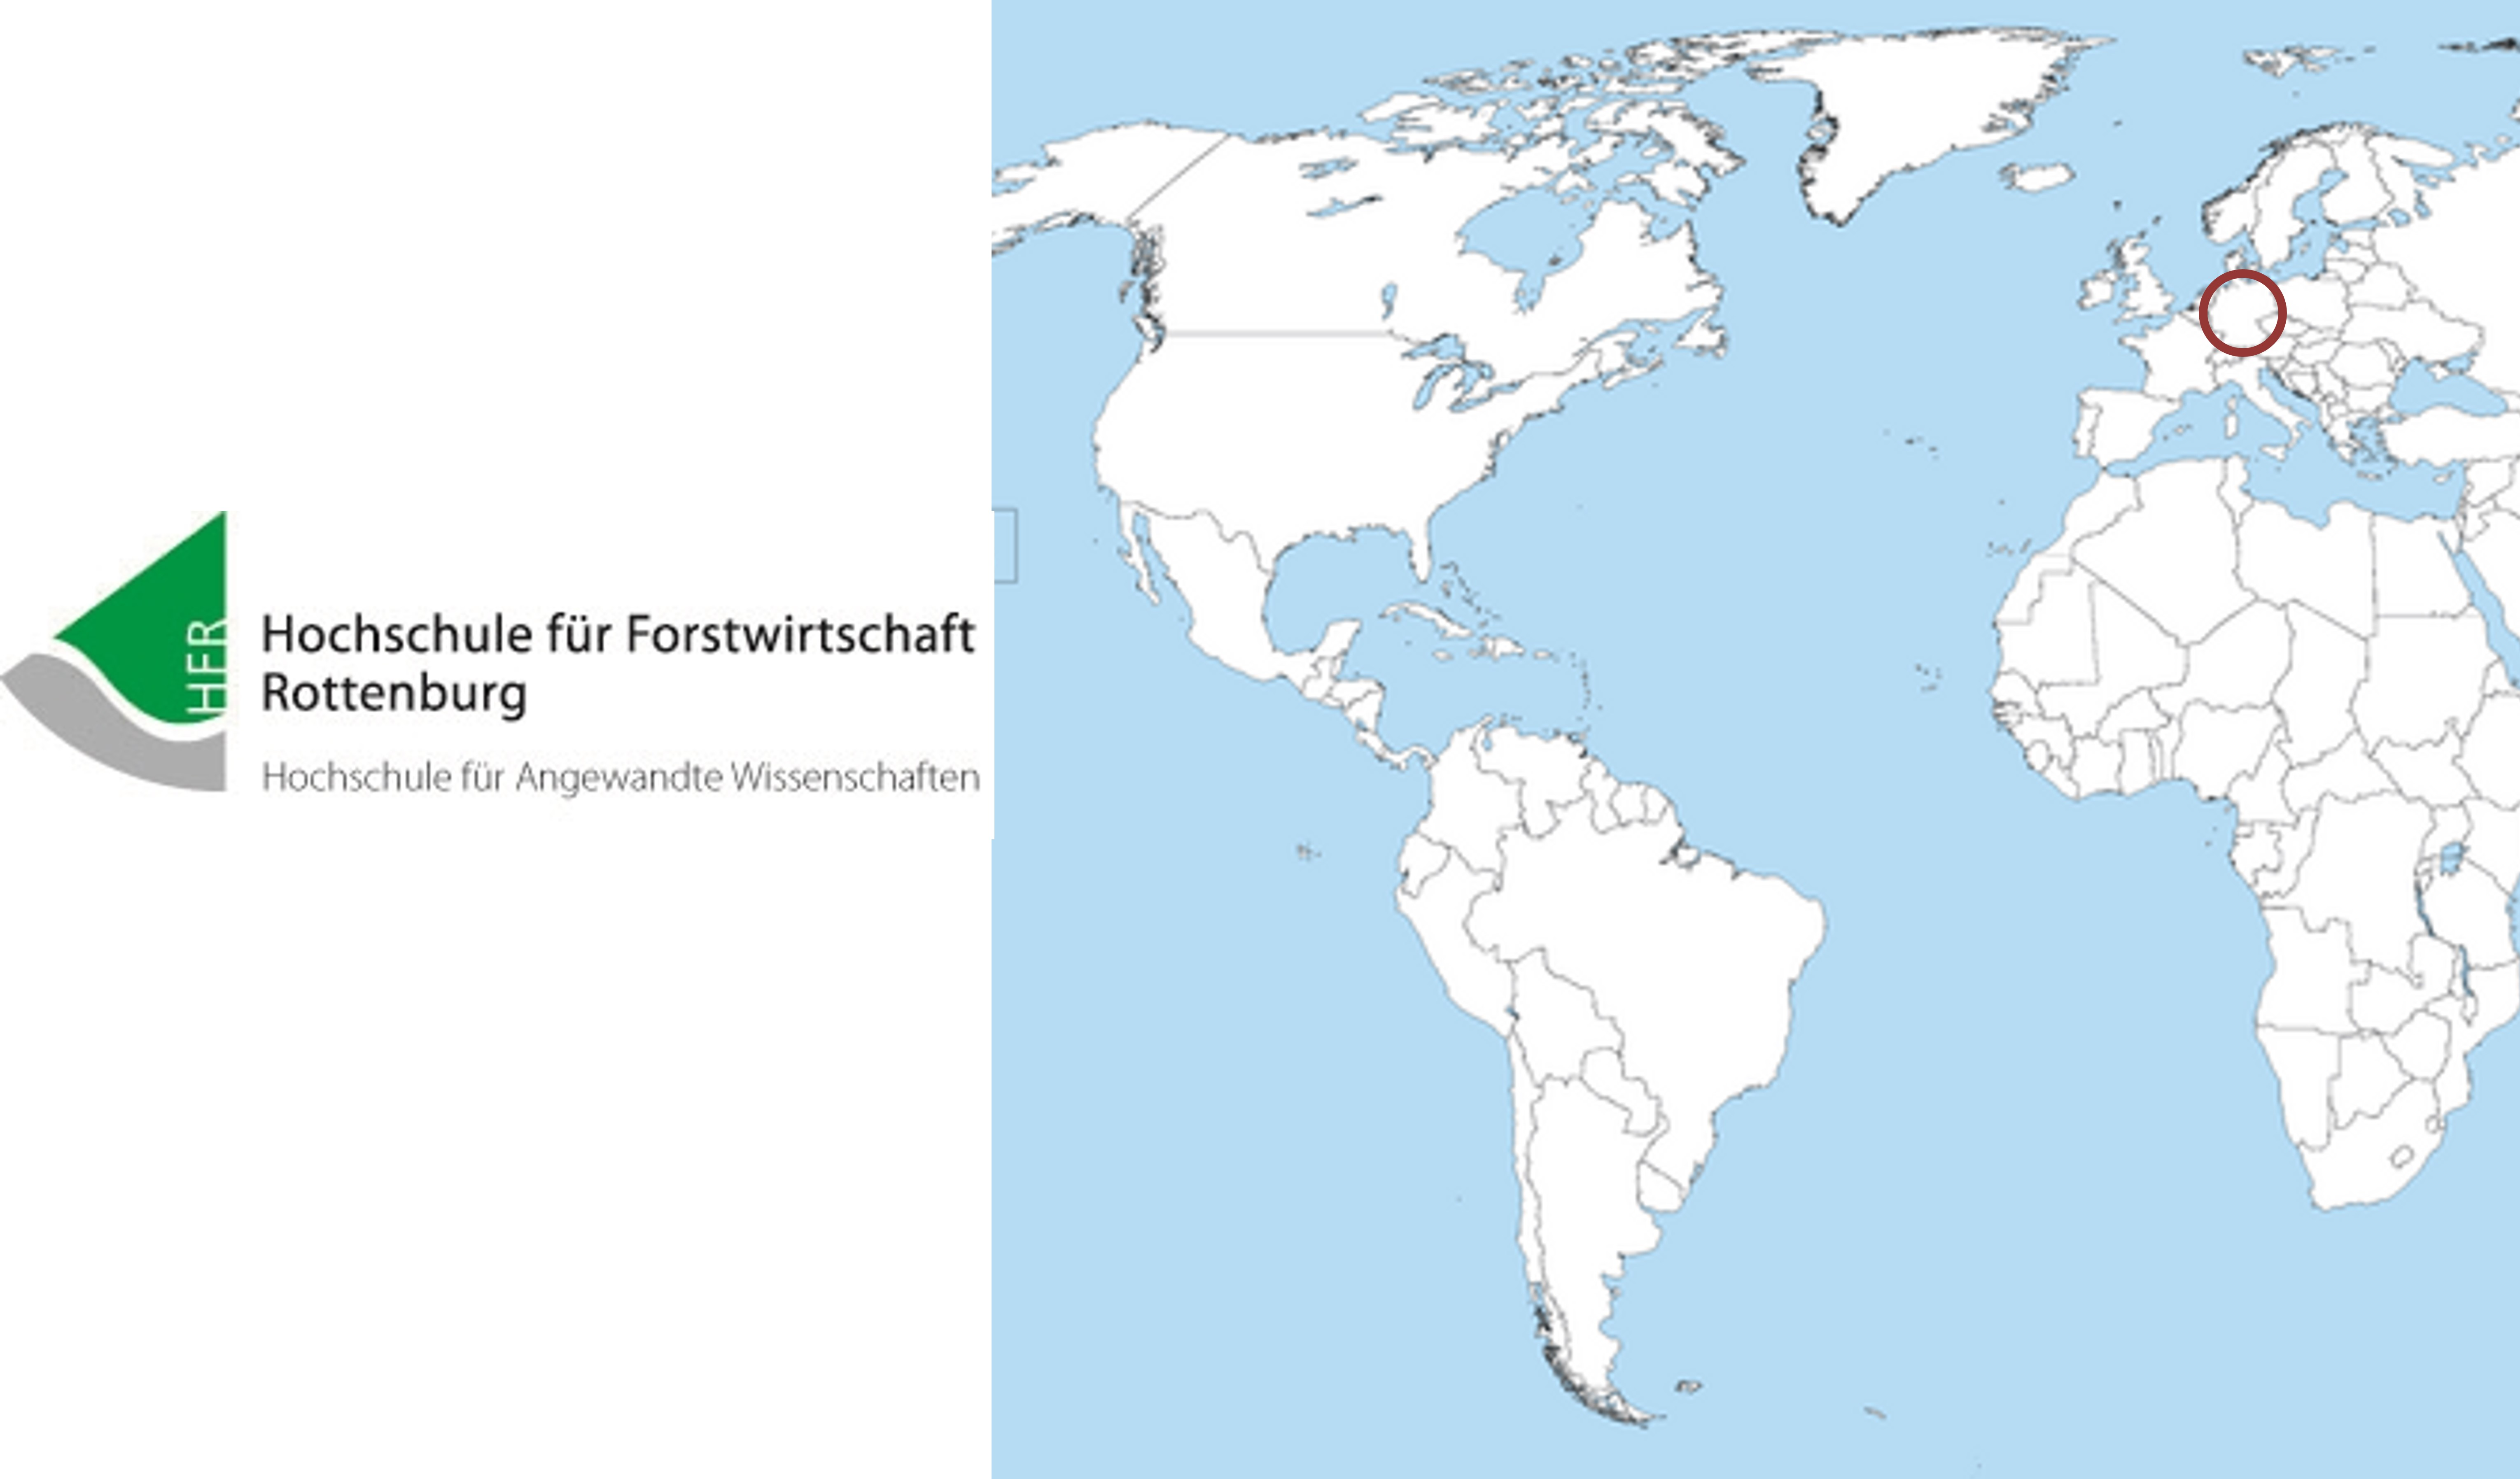
\includegraphics[width = 10cm, height = 4.5cm]{pic/germany.jpg}
       \end{figure}
\end{frame}

\begin{frame}{Personal background}
PhD
\begin{itemize}
    \item Assessment of the uncertainty from different sources in forest inventories
    \item hybrid estimators
    \item volume and biomass
    \item Team: Professors Sylvio, Alexandre, Rubén
\end{itemize}

\begin{figure}
        \centering
        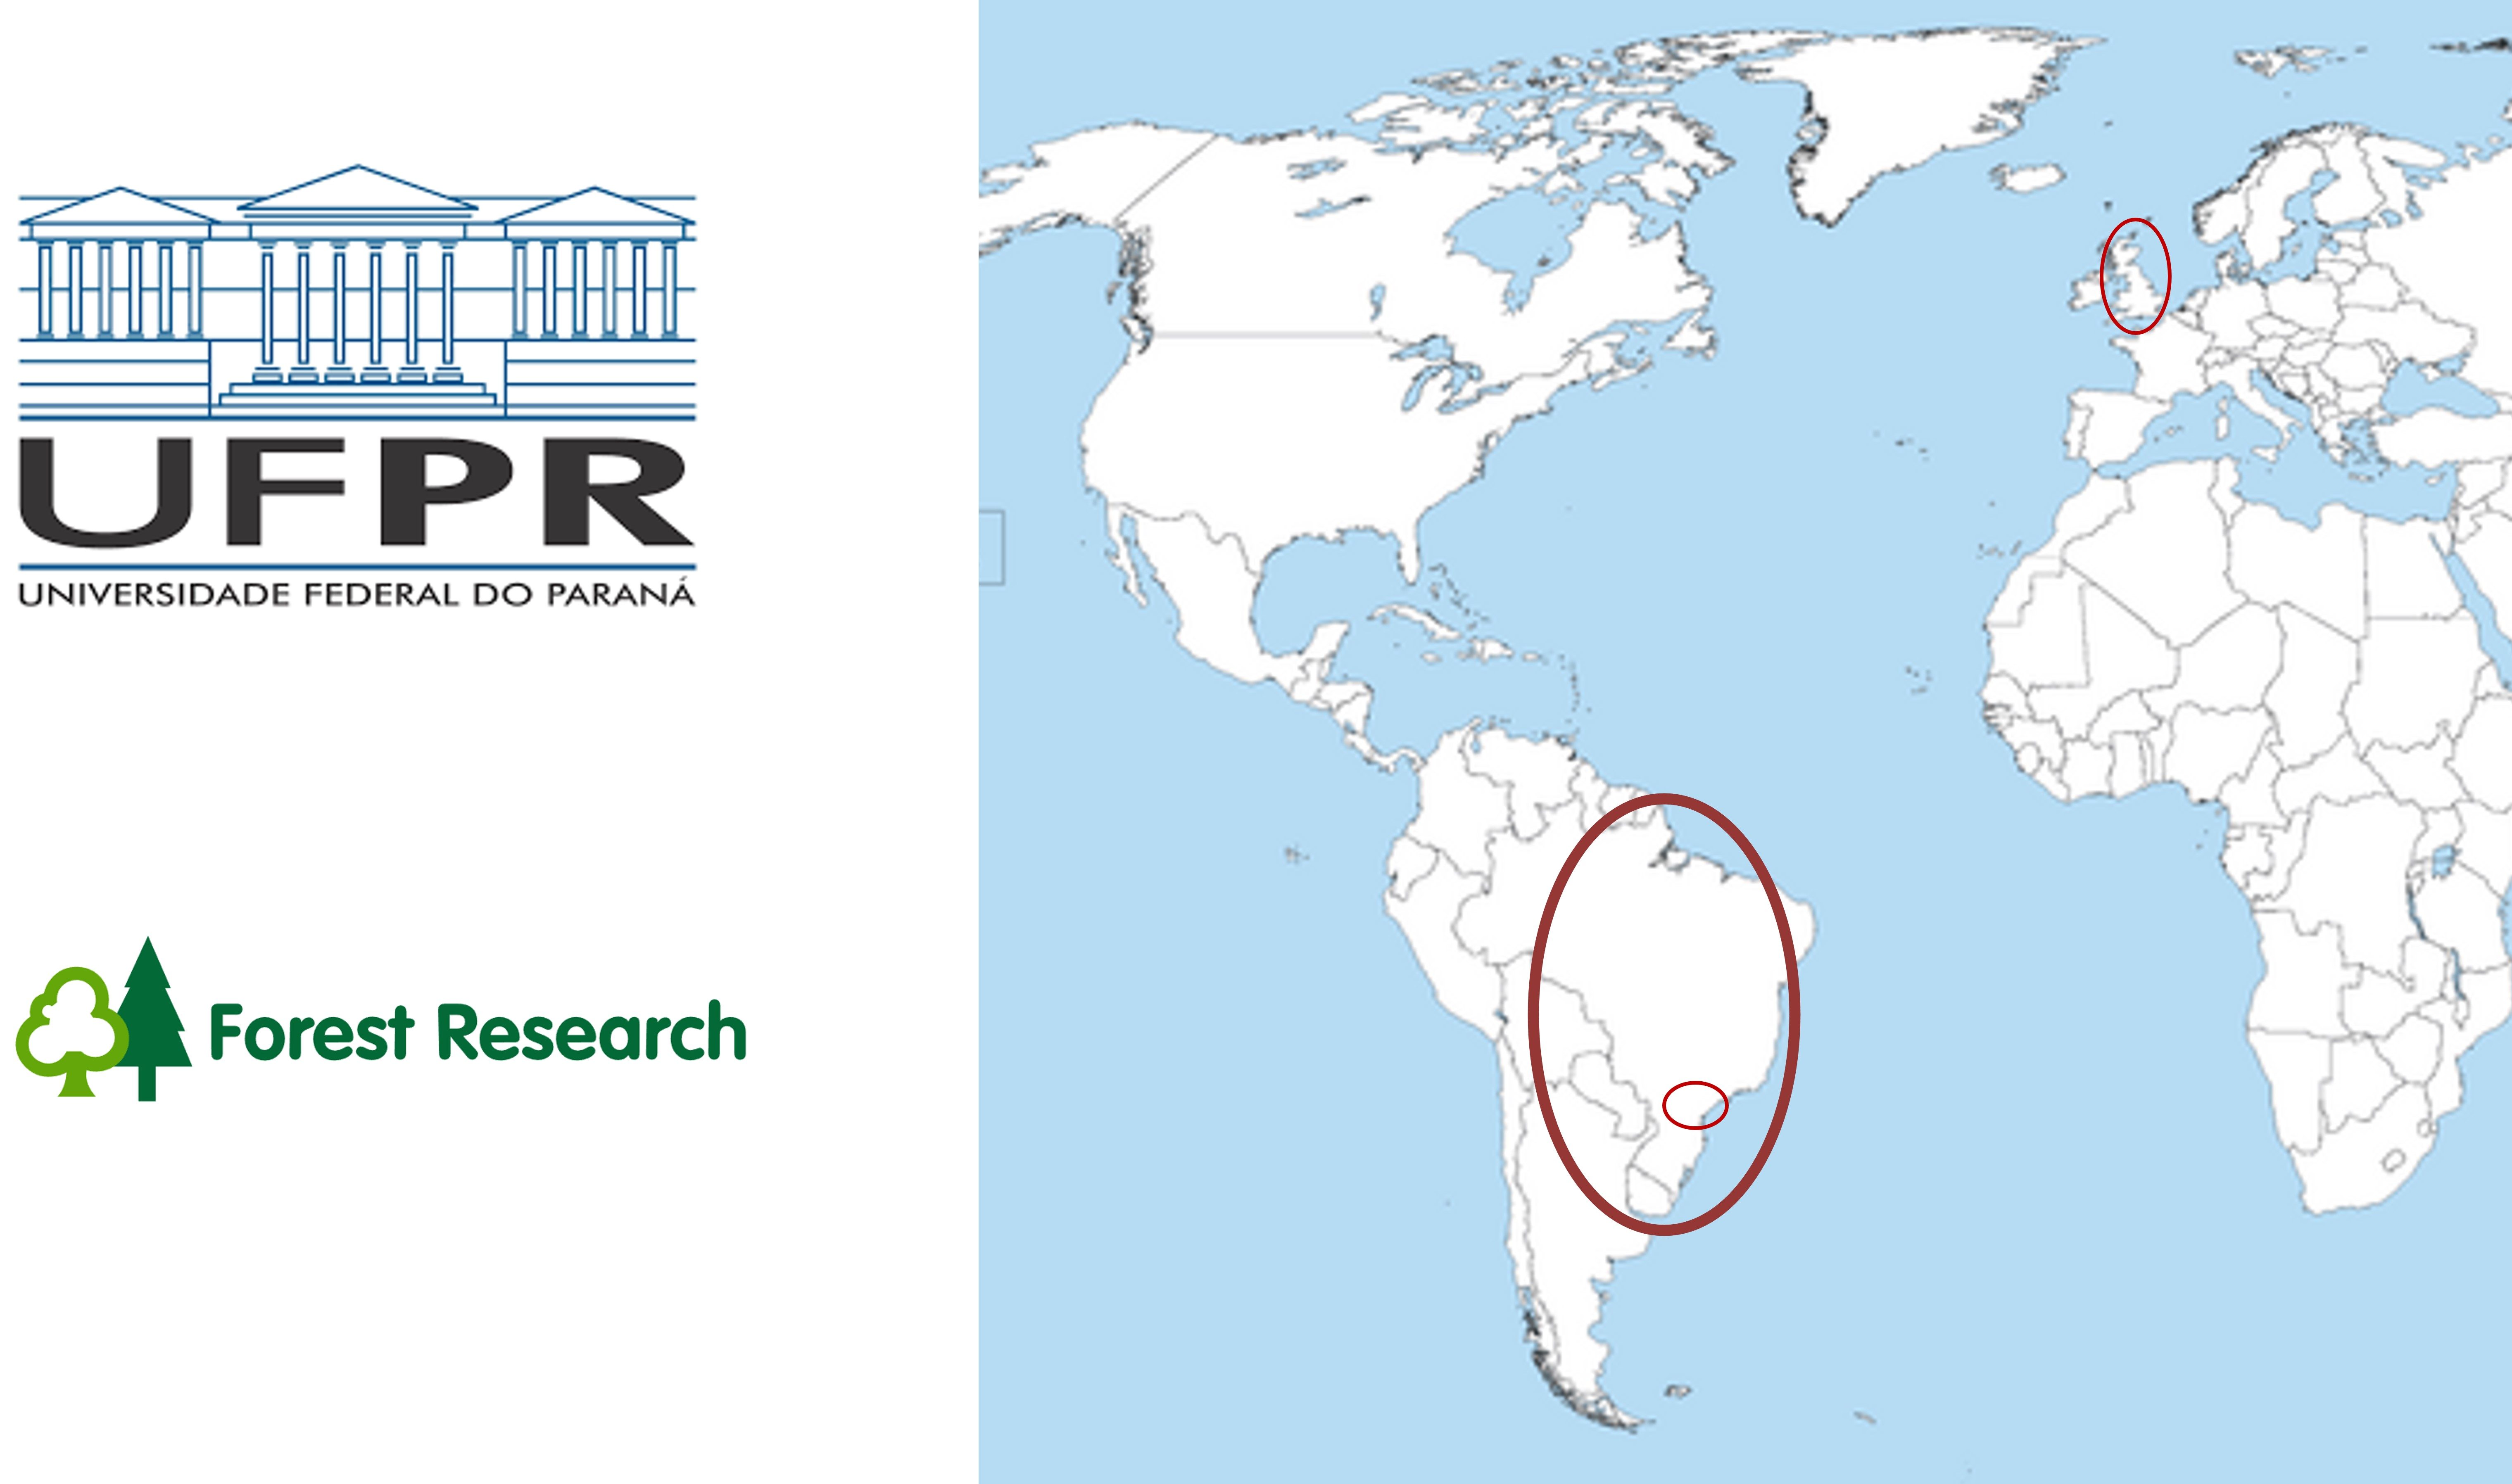
\includegraphics[width = 10cm, height = 4.5cm]{pic/vrasil-uk.jpg}
       \end{figure}
\end{frame}

\begin{frame}{Personal background}
Master:
\begin{itemize}
    \item Competition between trees
    \item different densities
    \item forest inventory
    \item Team: Professors Sylvio, Alexandre
\end{itemize}


\begin{figure}
        \centering
        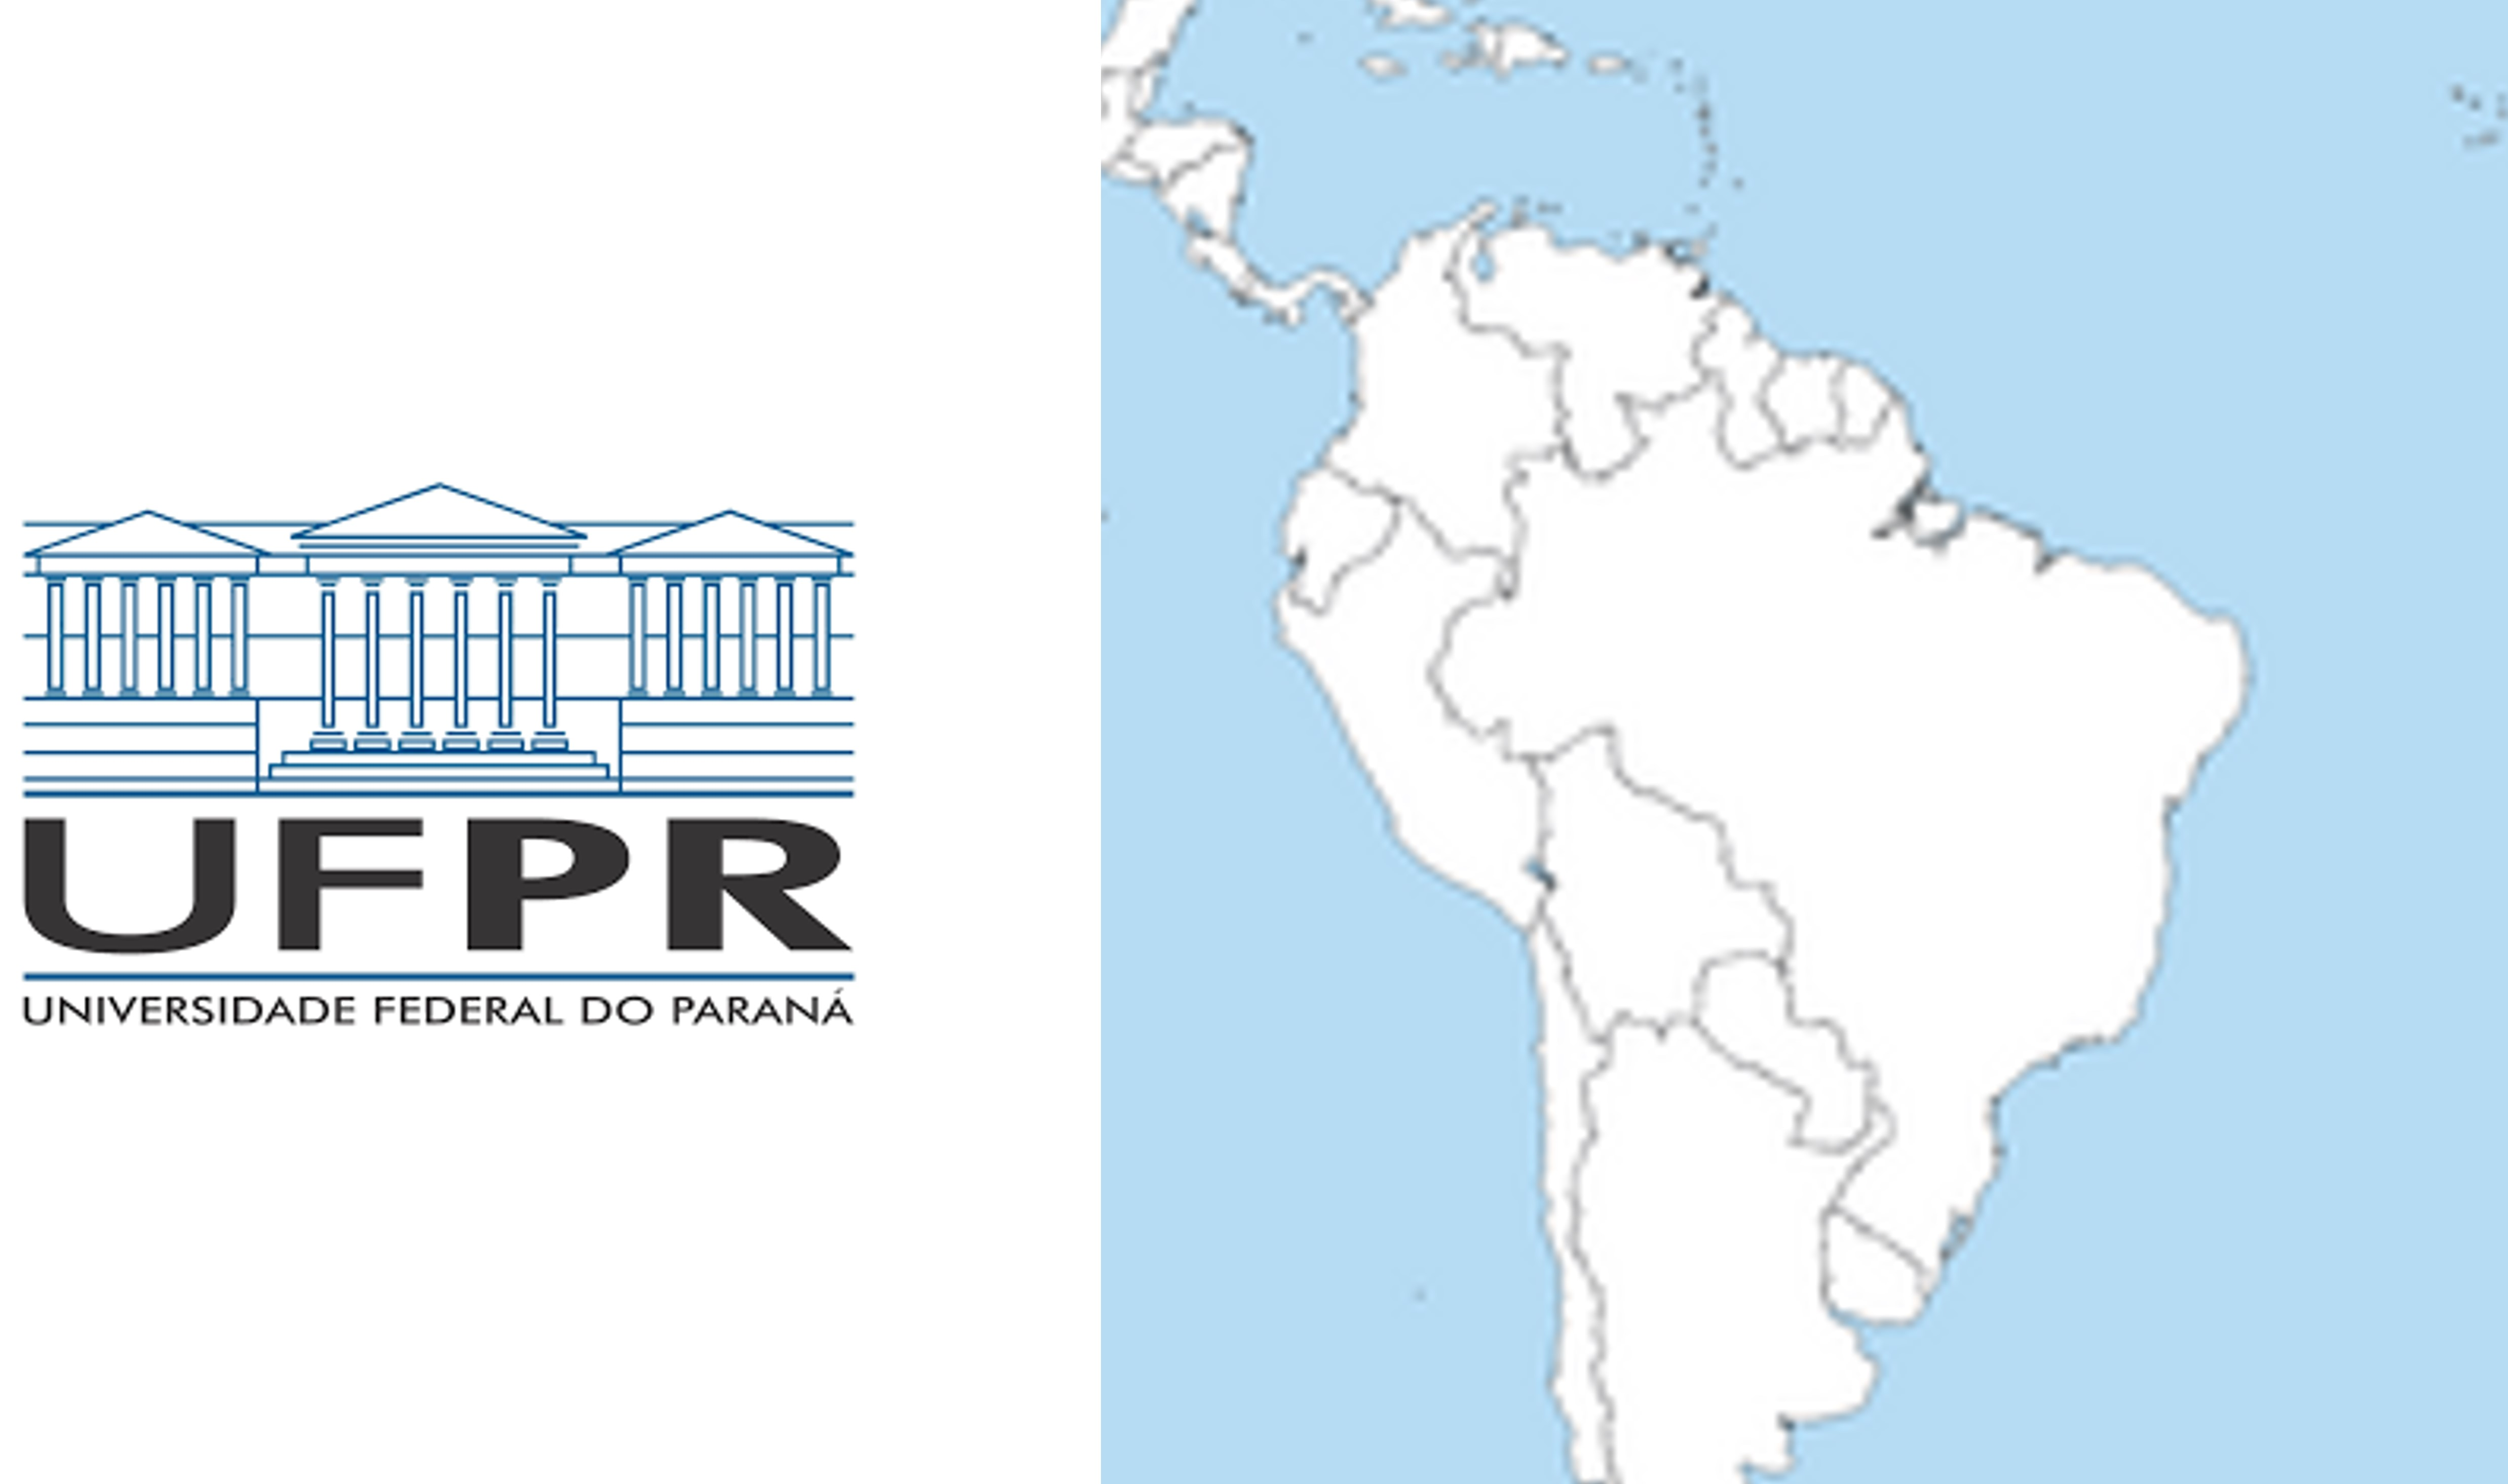
\includegraphics[width = 10cm, height = 4.5cm]{pic/curitiba.jpg}
       \end{figure}
\end{frame}

\begin{frame}{Introduction}
\begin{itemize}
    \item Why is there uncertainty in forest estimates?
\end{itemize}
\end{frame}

\begin{frame}{Introduction}
\begin{figure}
        \centering
        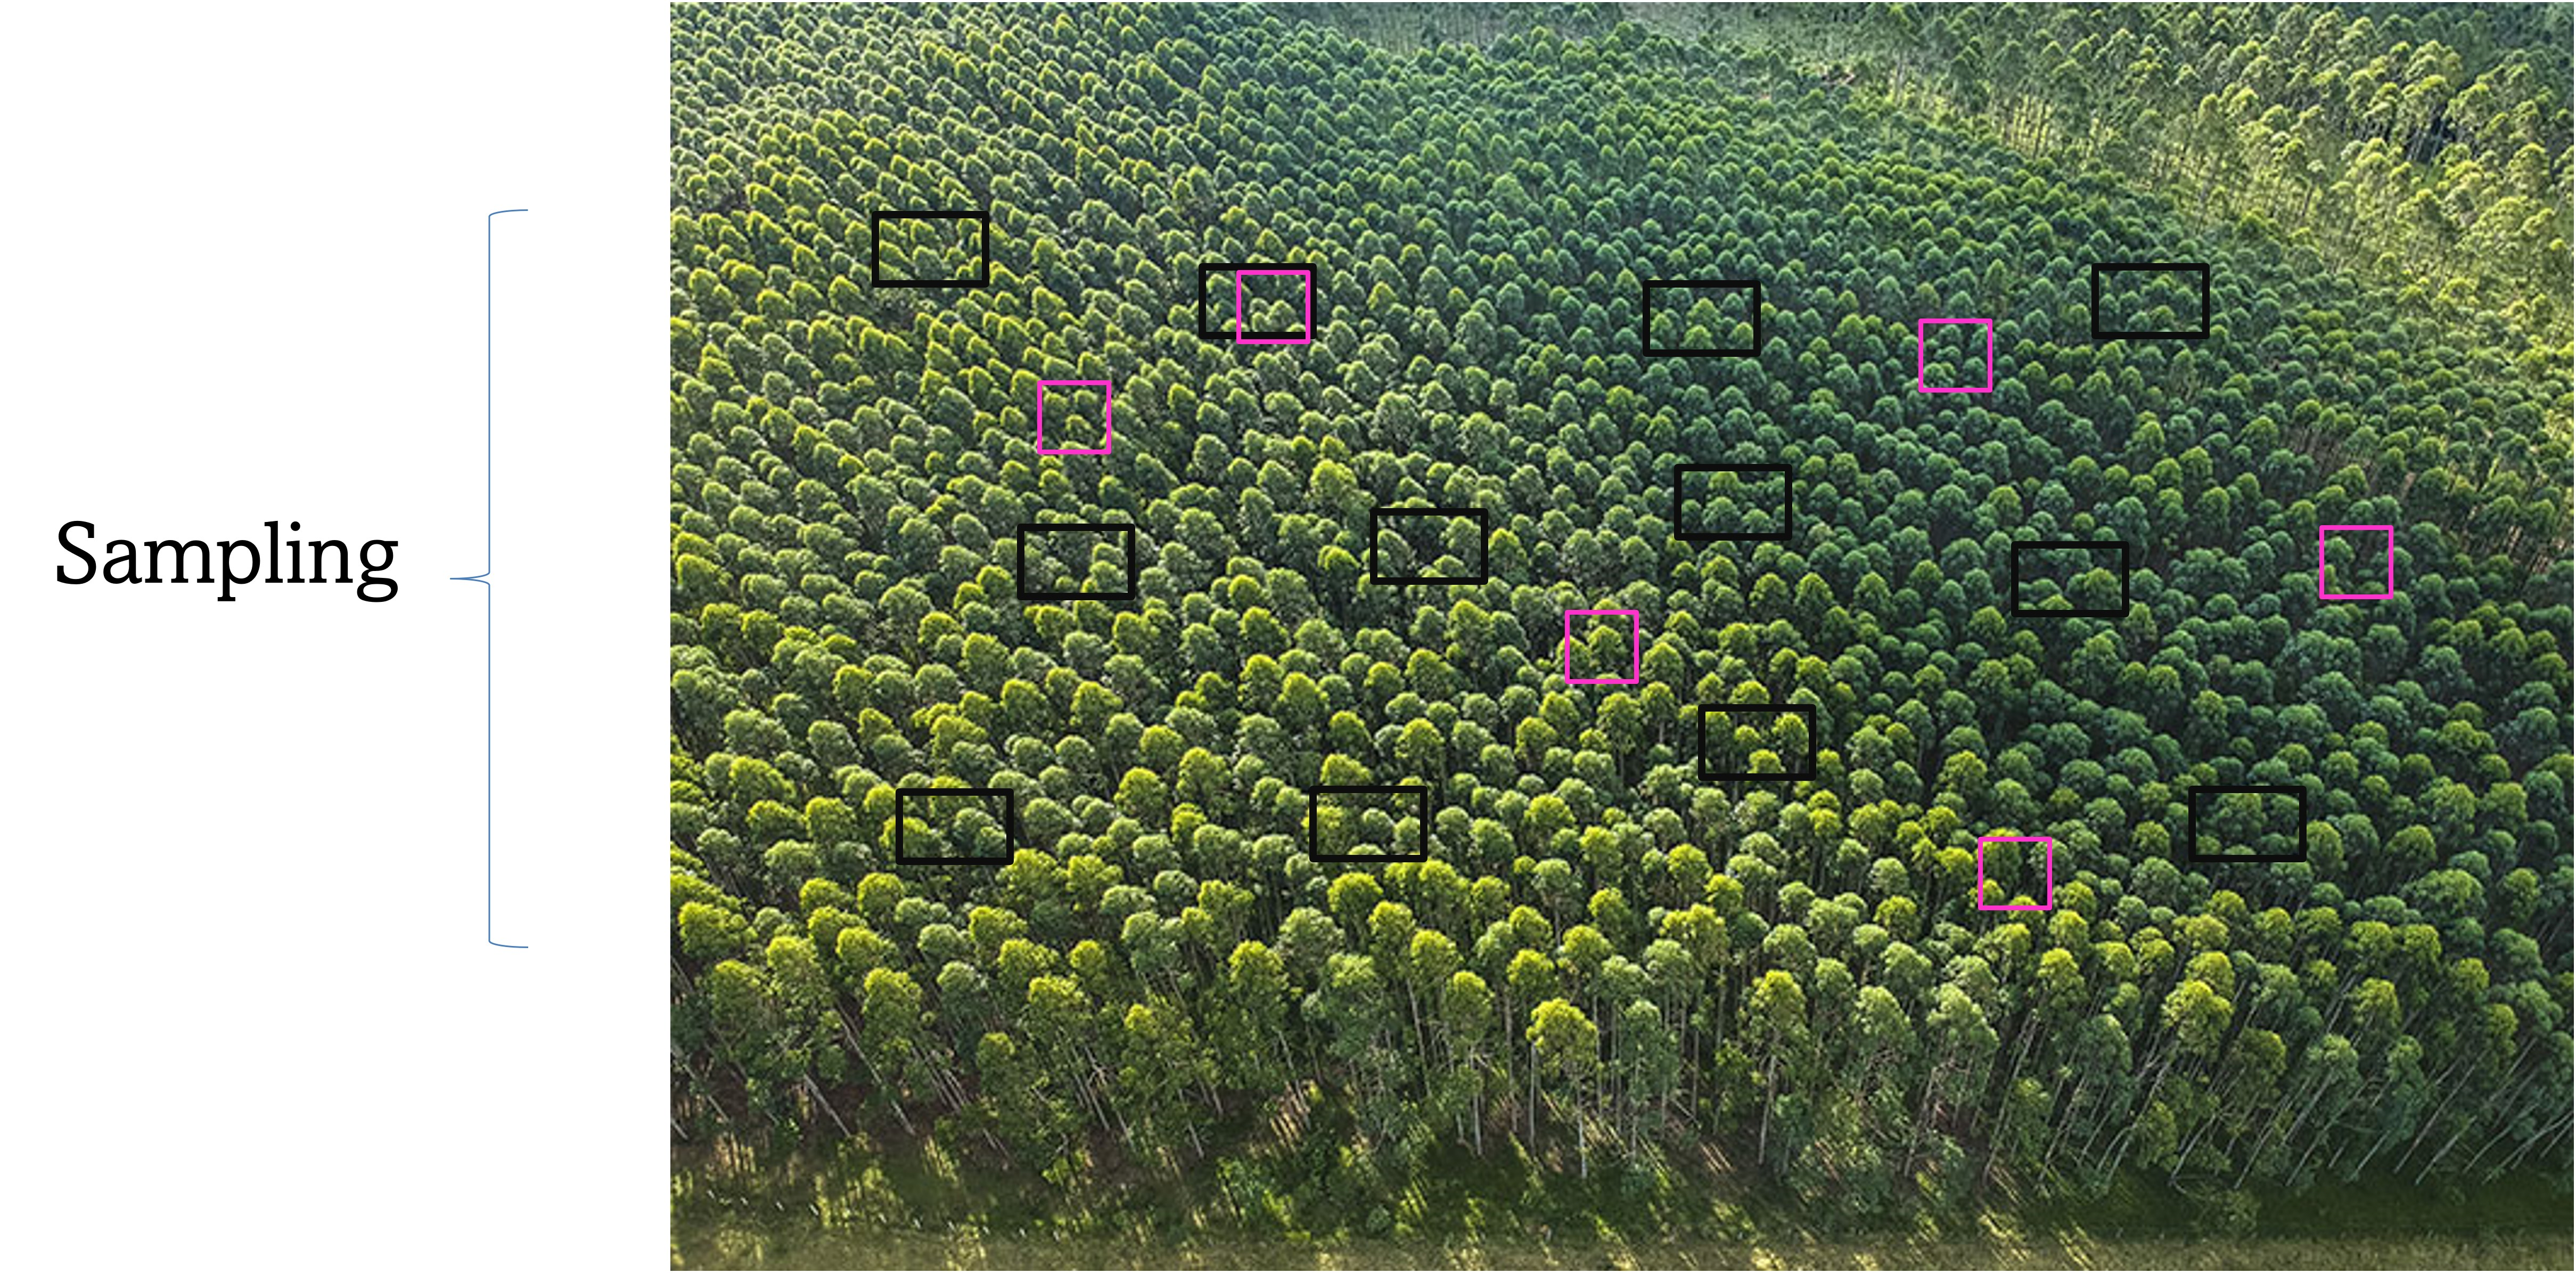
\includegraphics[width = 10cm, height = 5cm]{pic/Imagem1.jpg}
        \end{figure}
\begin{itemize}
    \item Inability to measure the variables of interest across the population.
    \item Random variability around a measurement, estimation or prediction as a result of unknown information.
\end{itemize}

\end{frame}

\begin{frame}{Introduction}
\begin{figure}
        \centering
        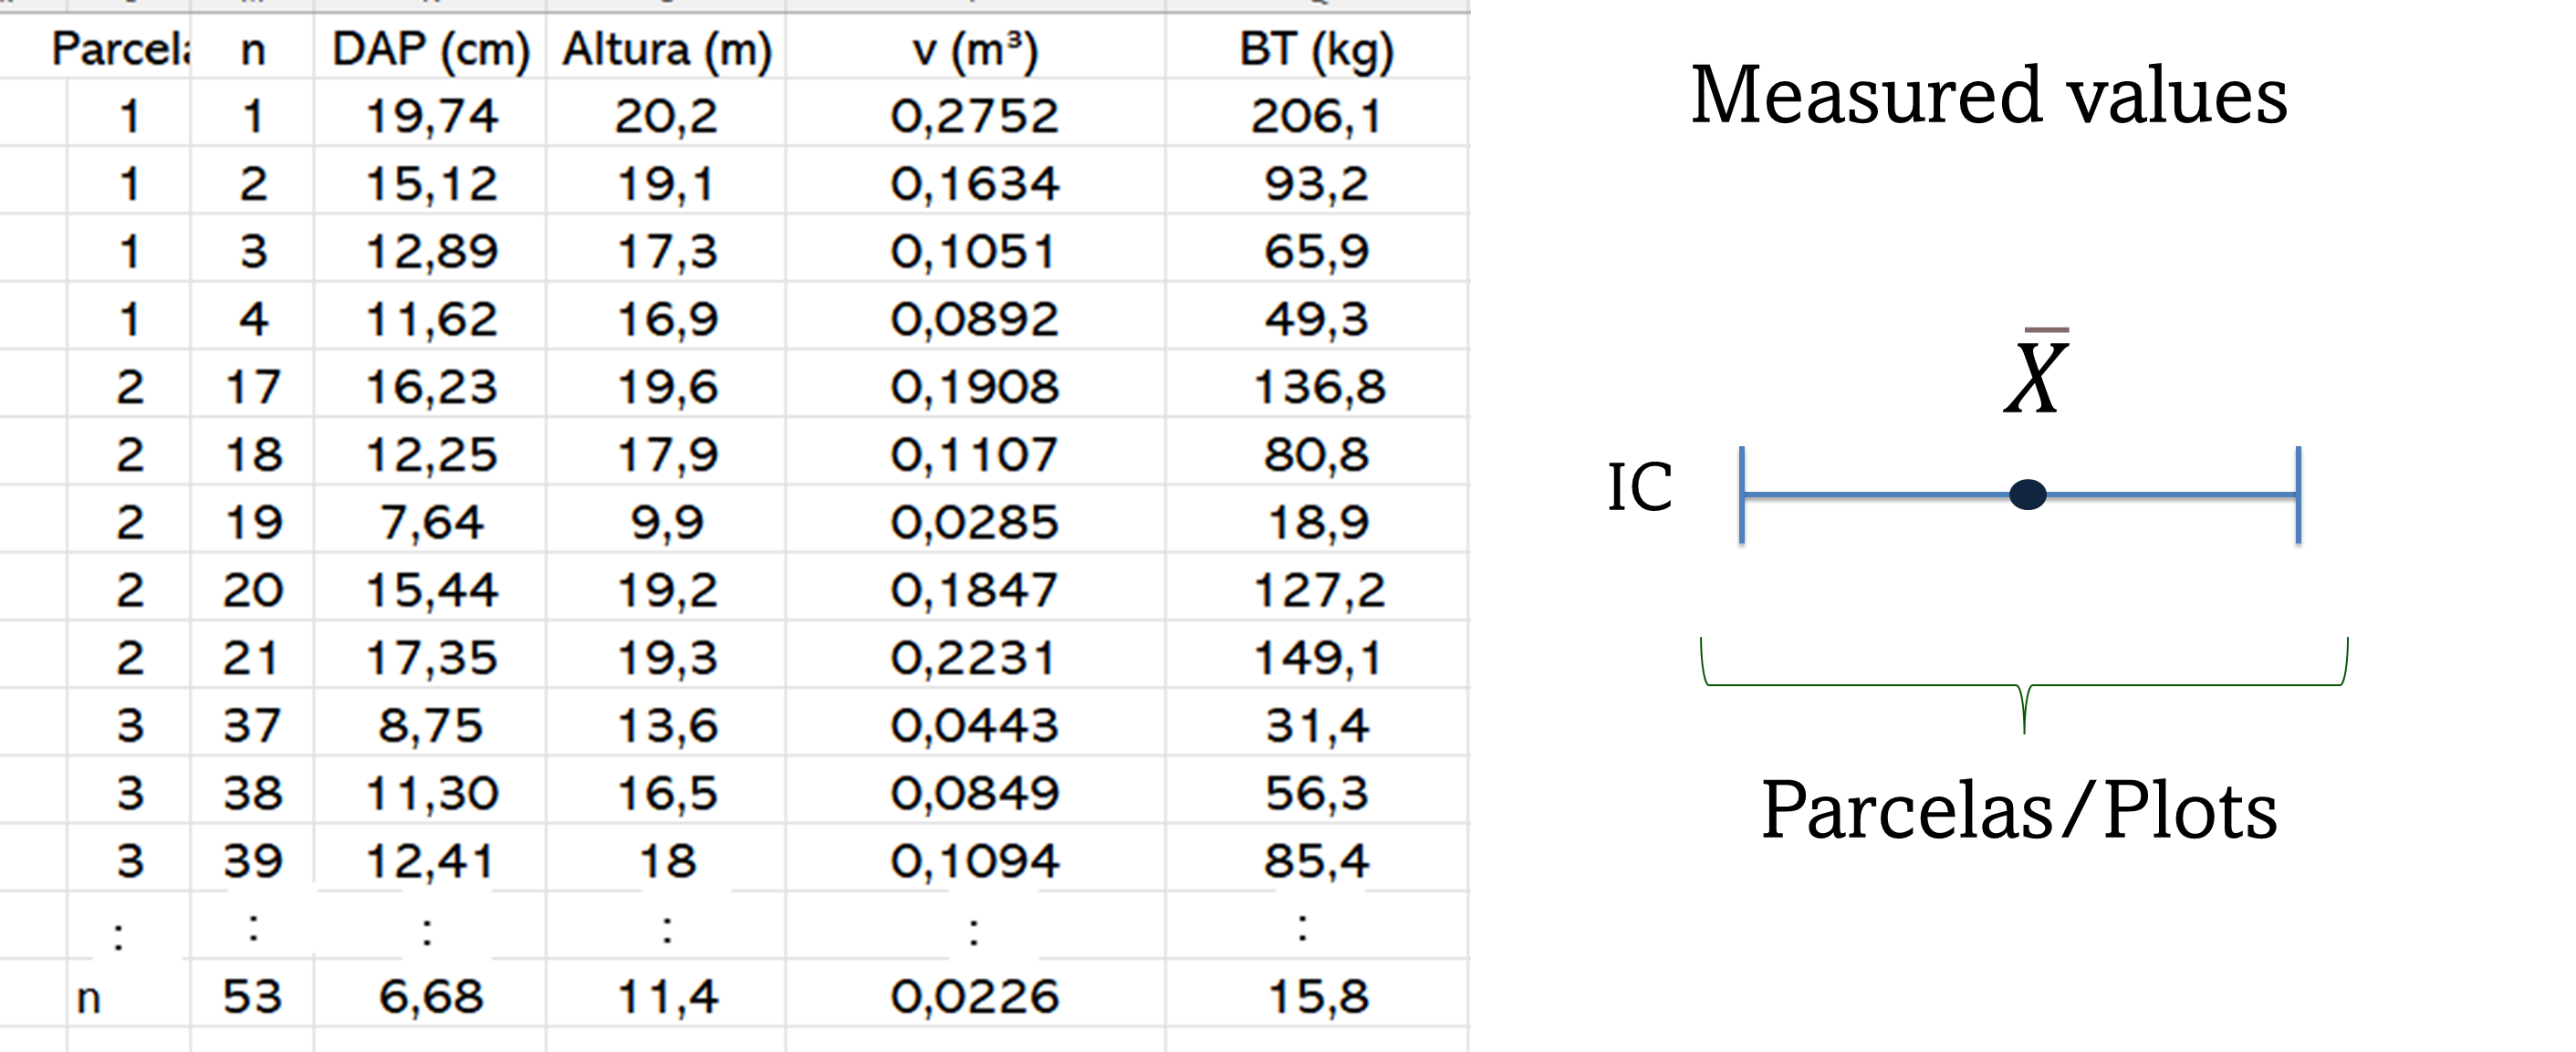
\includegraphics[width = 12cm, height = 5cm]{pic/Imagem2.png}
        \end{figure}
\begin{itemize}
    \item Inability to measure the variables of interest across the population.
\end{itemize}
\end{frame}

\begin{frame}{Introduction}
\begin{figure}
        \centering
        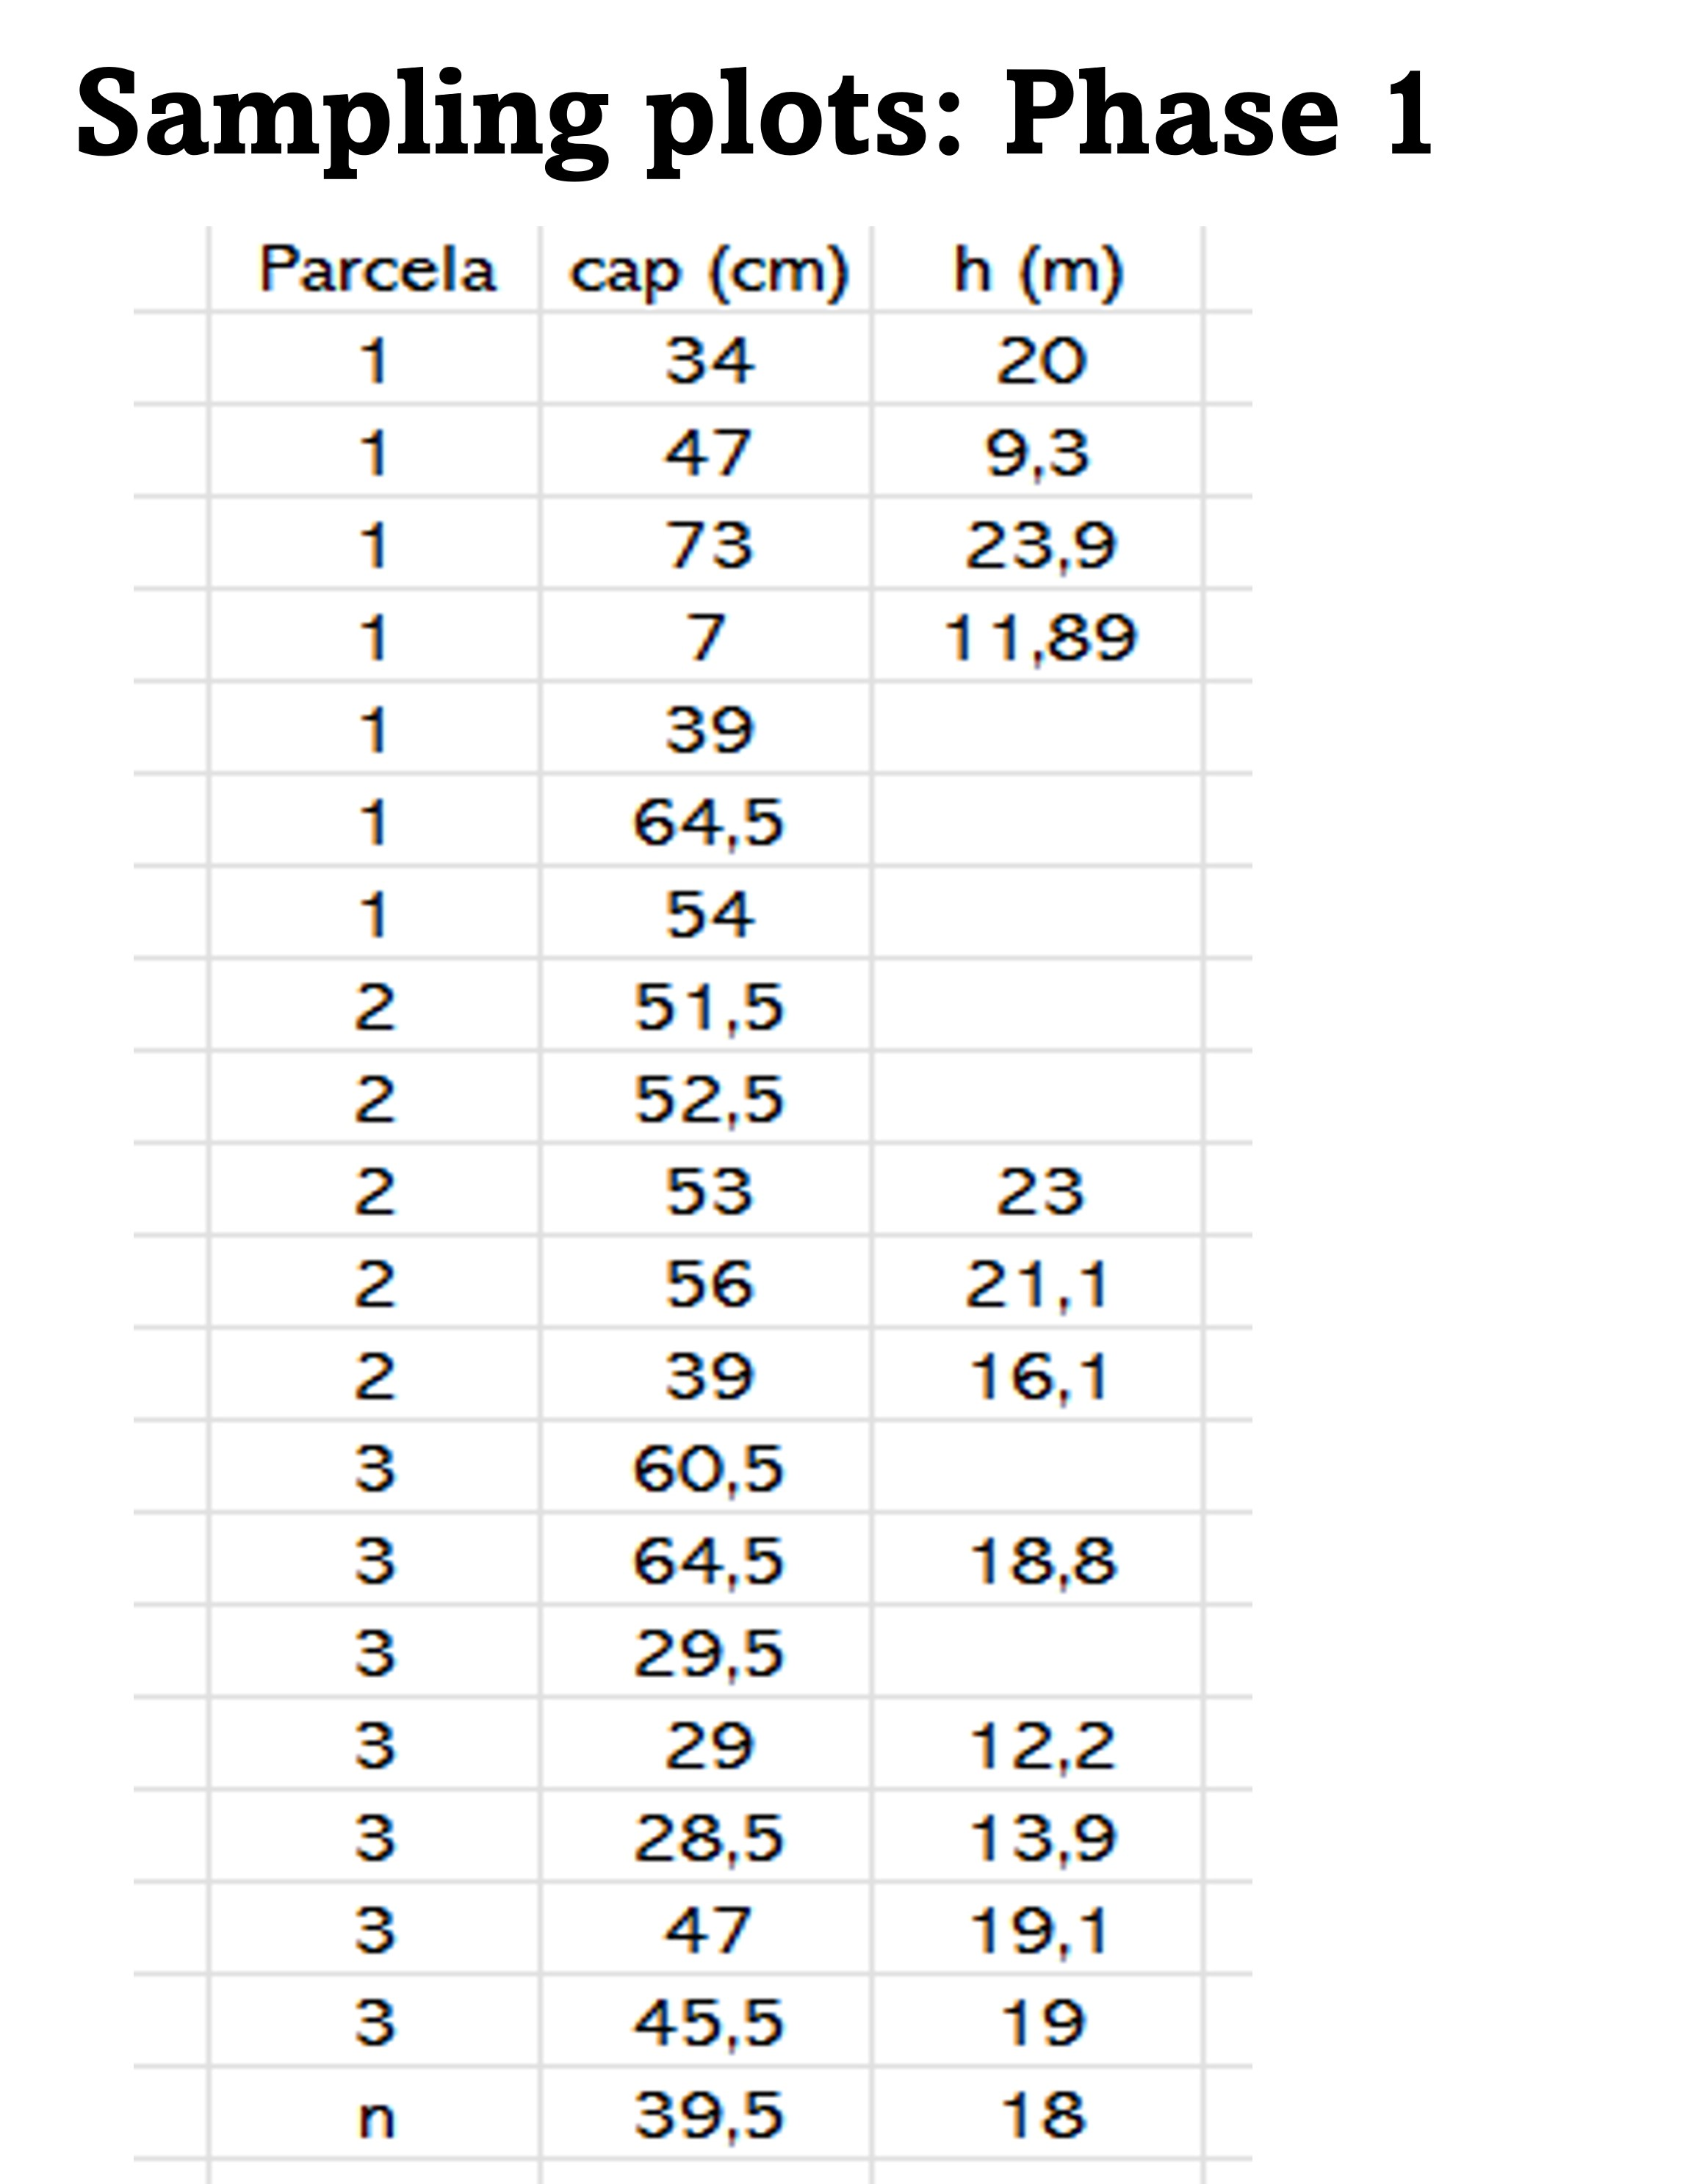
\includegraphics[width = 6cm, height = 6.2cm]{pic/imagem 3.jpg}
        \end{figure}
\begin{itemize}
    \item Inability to measure the variables of interest across the population.
\end{itemize}
\end{frame}

\begin{frame}{Introduction}
\begin{figure}
        \centering
        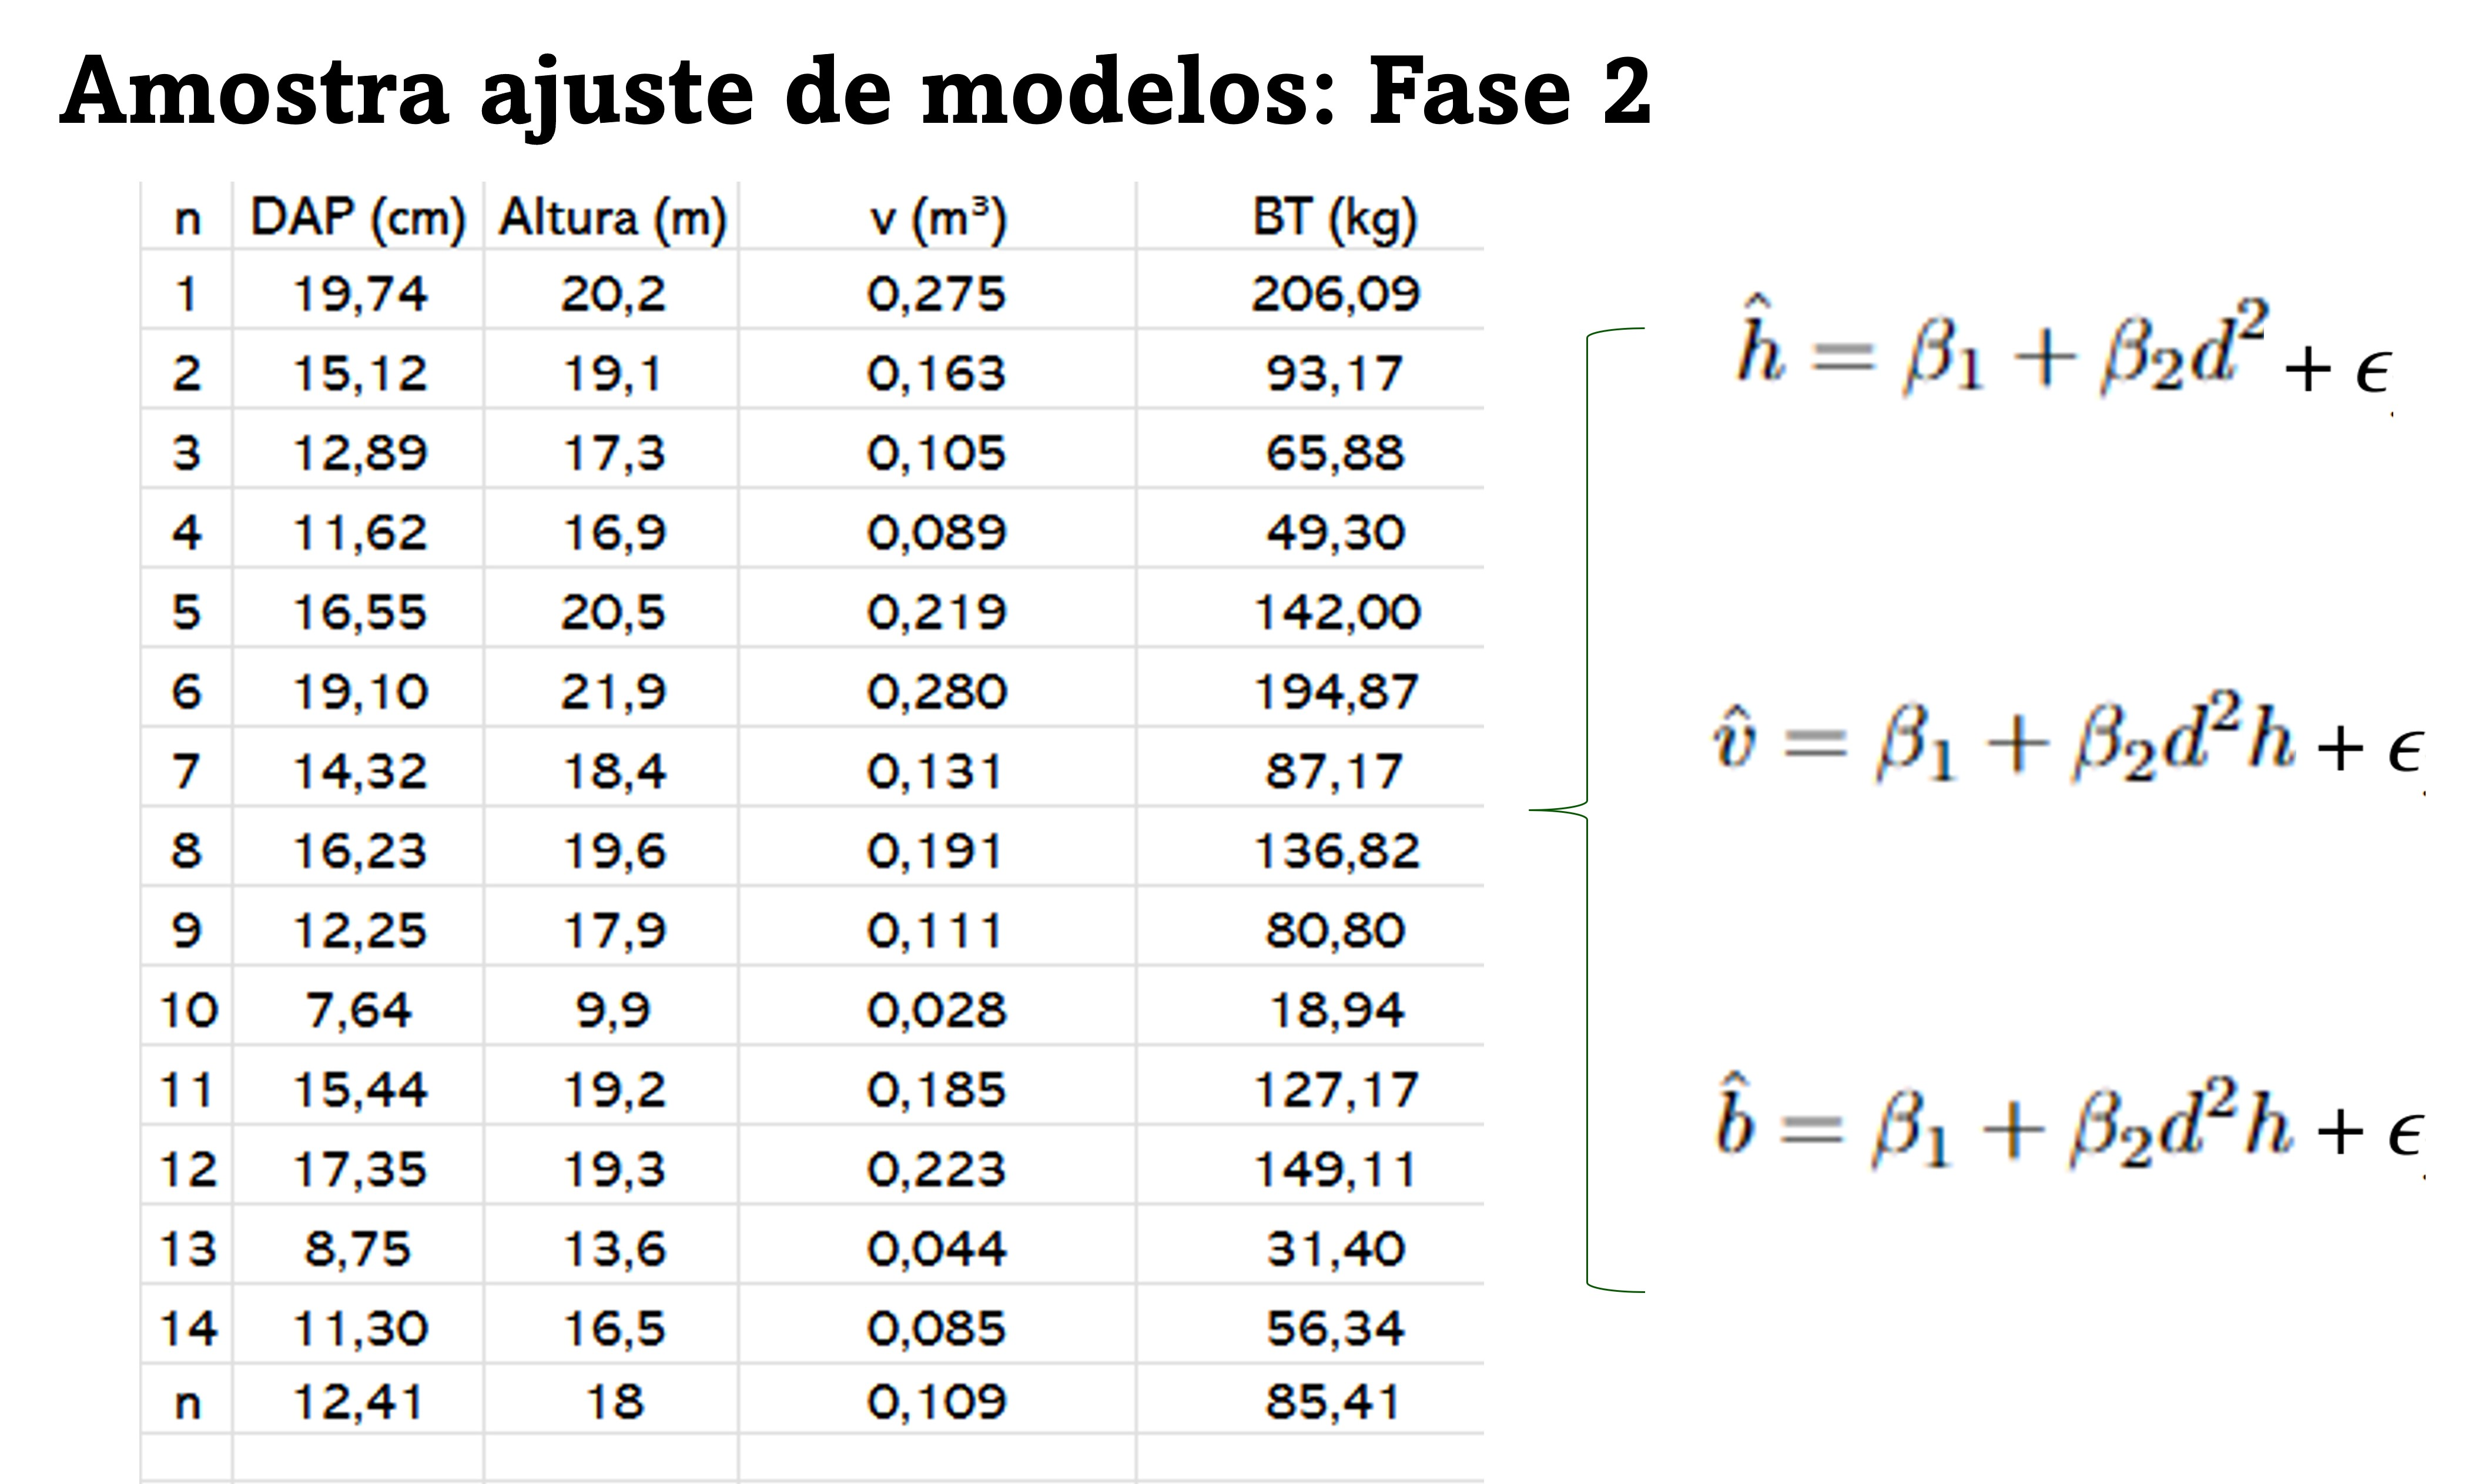
\includegraphics[width = 10cm, height = 6cm]{Imagem4.jpg}
        \end{figure}
\begin{itemize}
    \item Inability to measure the variables of interest across the population.
\end{itemize}
\end{frame}

\begin{frame}{Introduction}
\begin{figure}
        \centering
        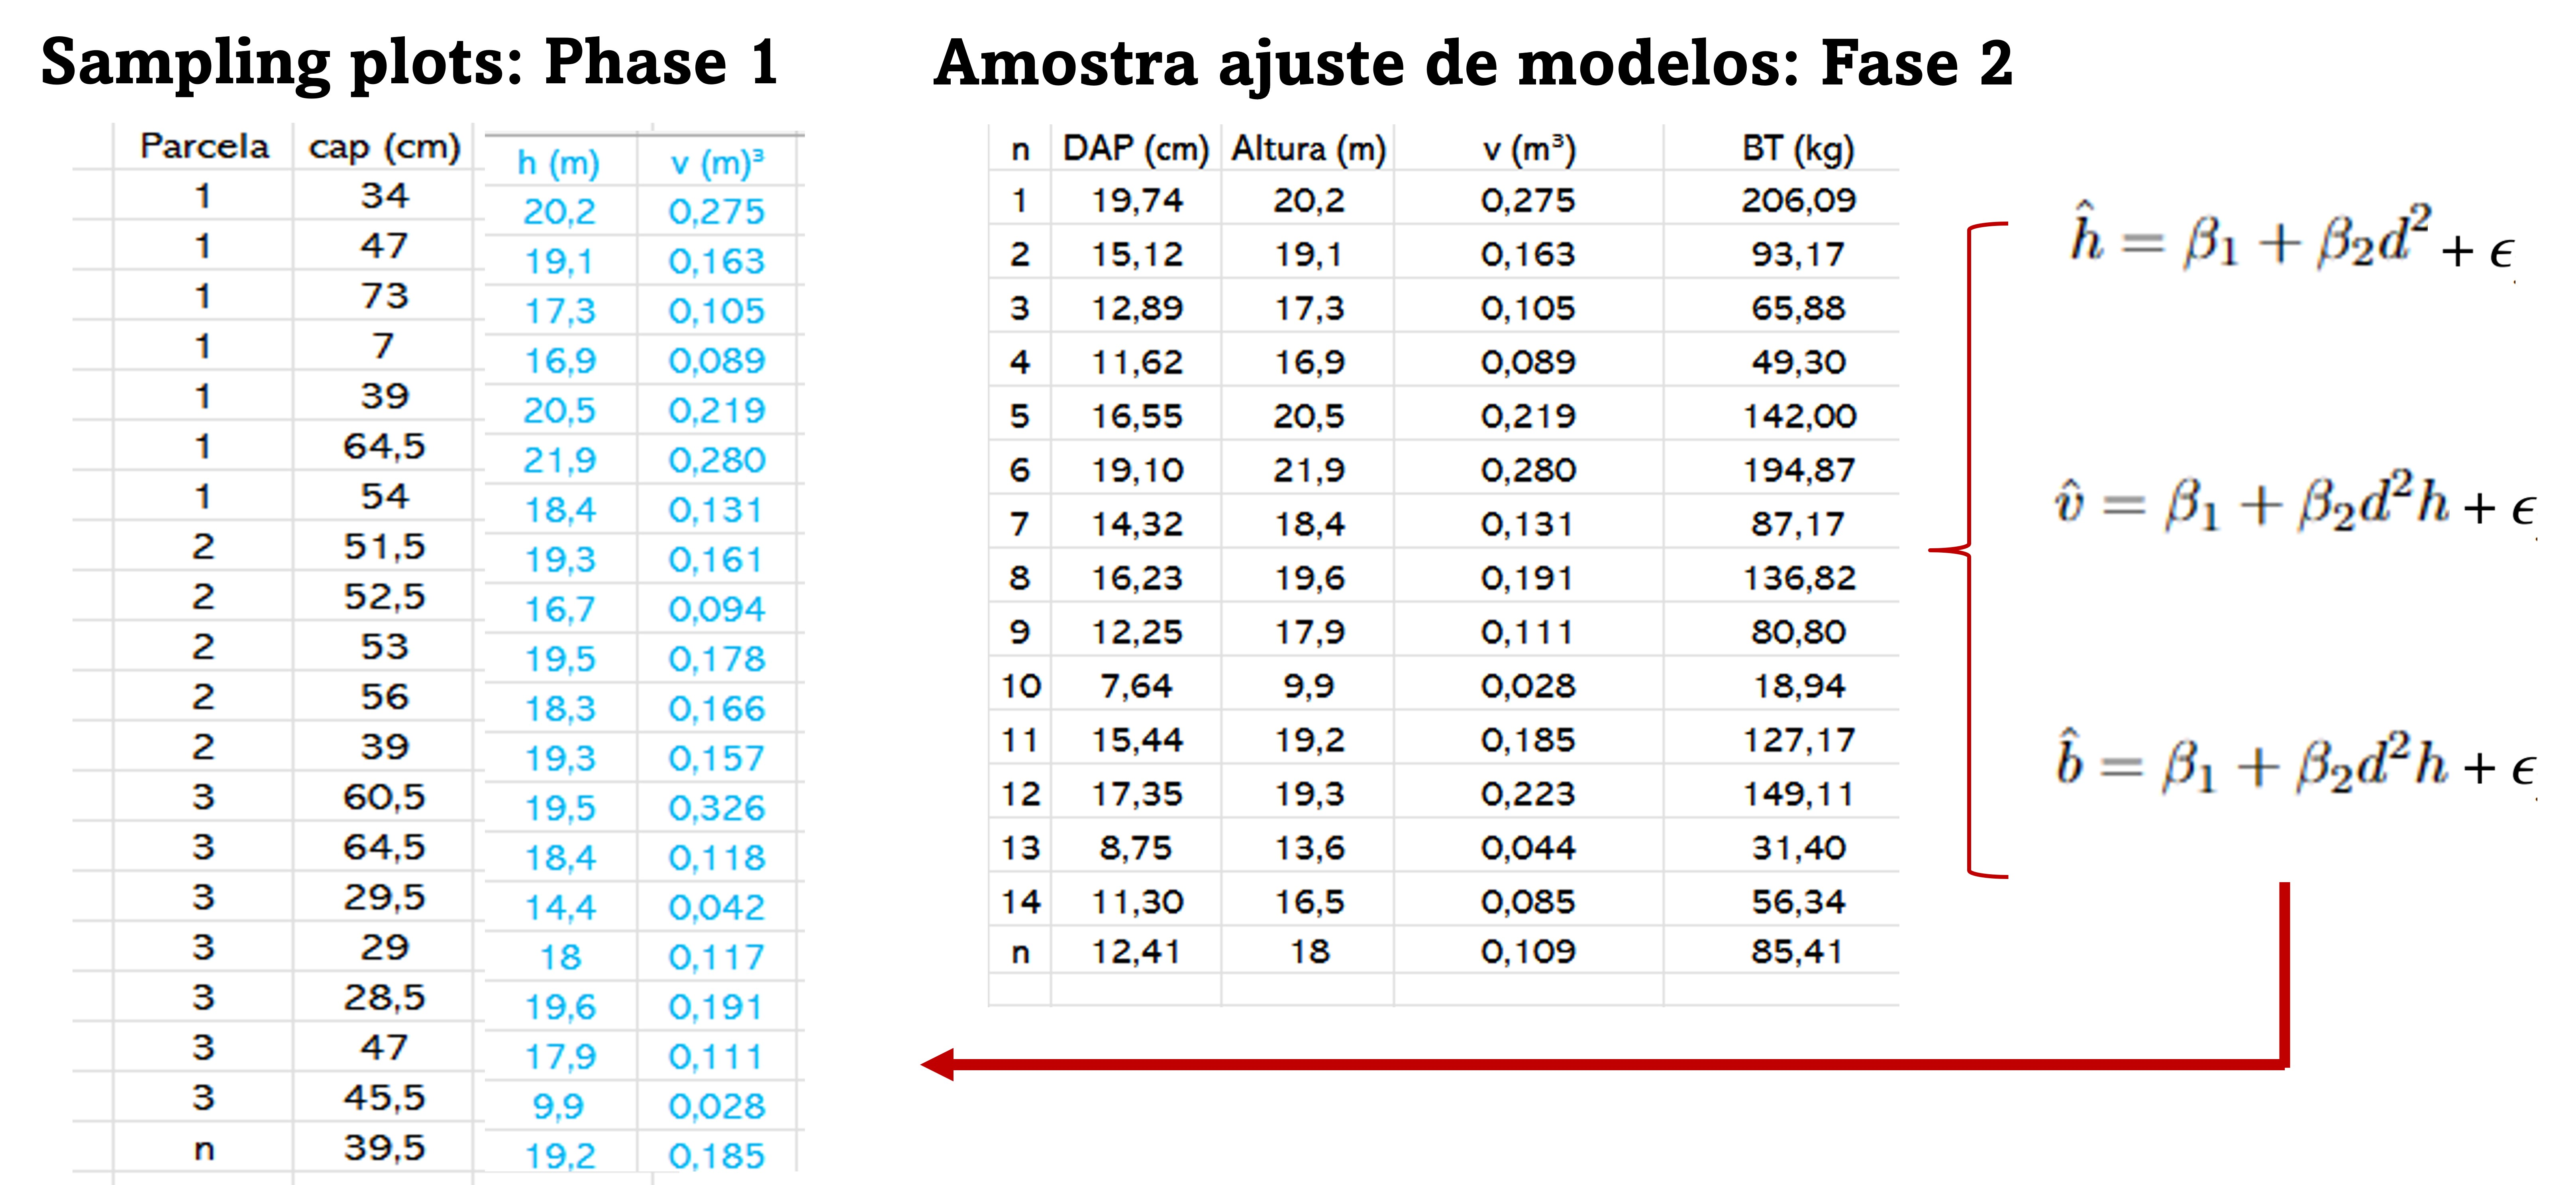
\includegraphics[width = 11cm, height = 5.5cm]{Imagem9.jpg}
        \end{figure}
\begin{itemize}
    \item Inability to measure the variables of interest across the population.
\end{itemize}
\end{frame}

\begin{frame}{Why should we not ignore uncertainty? }
Example
\begin{itemize}
    \item 100 $ha^{-1}$ forest 
    \item Management objectives: Timber extraction
    \item Management strategy: Not to cut if stand density is below 100 $m³/ha^{-1}$
    \item Forest inventory to determine current stand density
\end{itemize}
\begin{figure}
        \centering
        
\includegraphics[width = 12cm, height = 4cm]{pic/Imagem6.jpg}
        \end{figure}
\end{frame}

\begin{frame}{Why should we not ignore uncertainty?}
\begin{itemize}
    \item 100 $ha^{-1}$ forest 
    \item Management strategy: Not to cut if stand density is below 100 $m^3/ha^{-1}$
  \end{itemize}
\begin{figure}
        \centering
        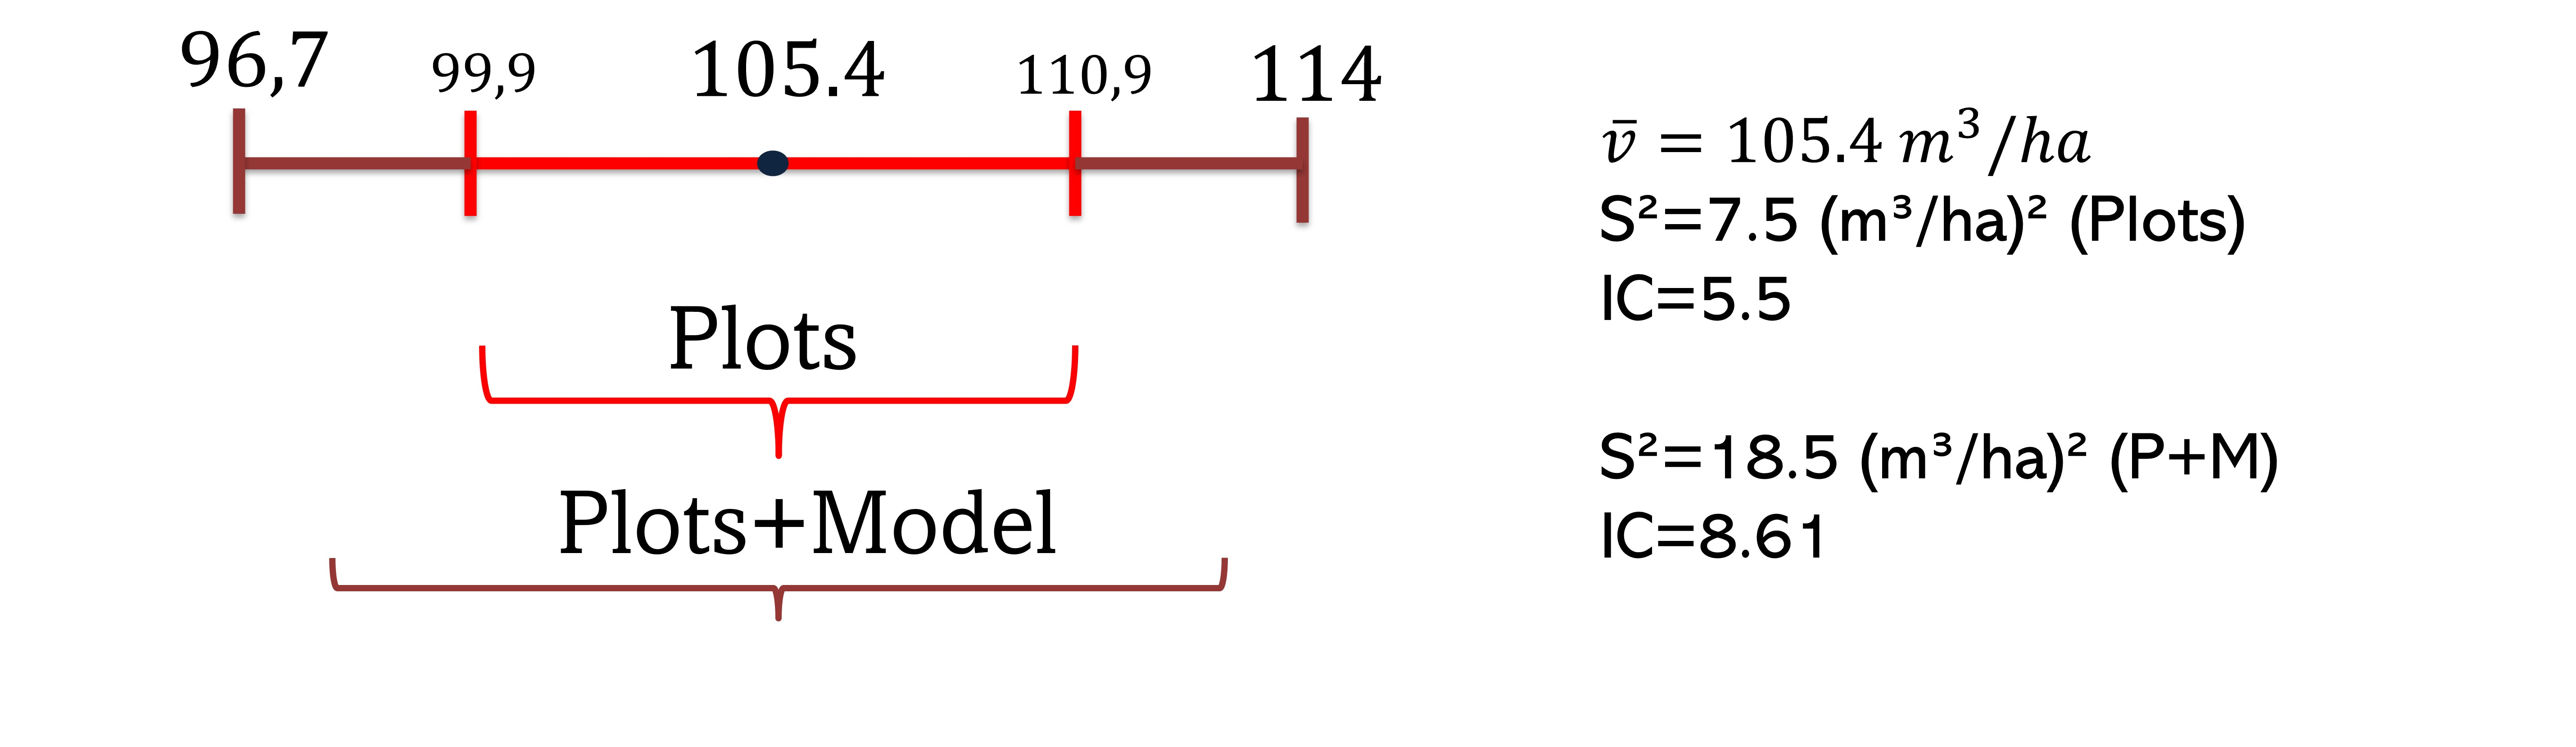
\includegraphics[width = 12cm, height = 4cm]{pic/exemplo.jpg}
        \end{figure}

95$\%$ probability that the true 
value $(\mu )$ is within the confidence 
interval
\end{frame}

\begin{frame}{Why should we not ignore uncertainty?}
\begin{figure}
        \centering
        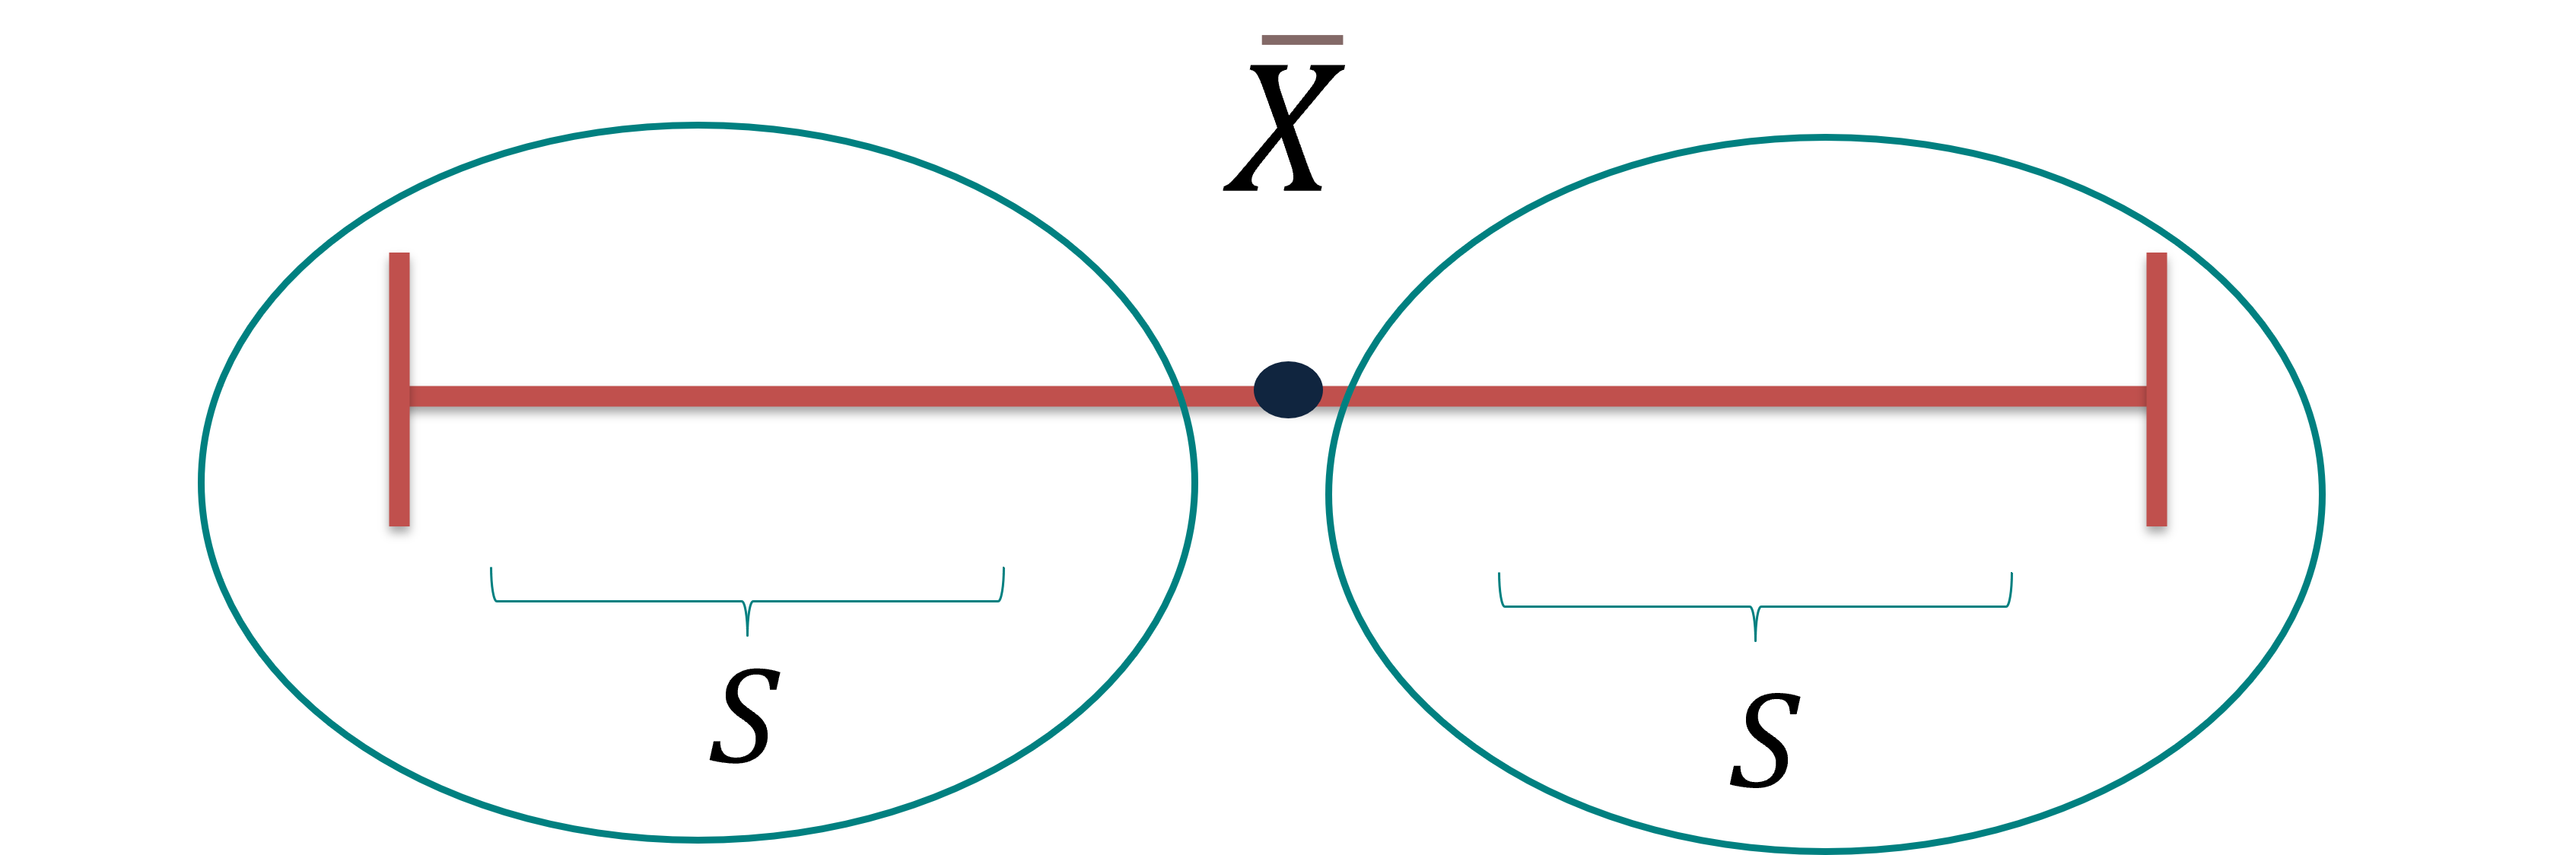
\includegraphics[width = 12cm, height = 4cm]{Imagem7.jpg.png}
        \end{figure}
\begin{itemize}
    \item Two main pieces of information from the inventory.
    \item Properly establish the confidence segment around the mean.
\end{itemize}
\end{frame}

\section{Uncertainty Sources}
\begin{frame}{Uncertainty Sources}

\begin{itemize}
    \item Sampling selection. Plot size, shape and number.
    \item Model: Sampling selection.
    \item Landscape-level heterogeneity
\end{itemize}
\begin{figure}
        \centering
        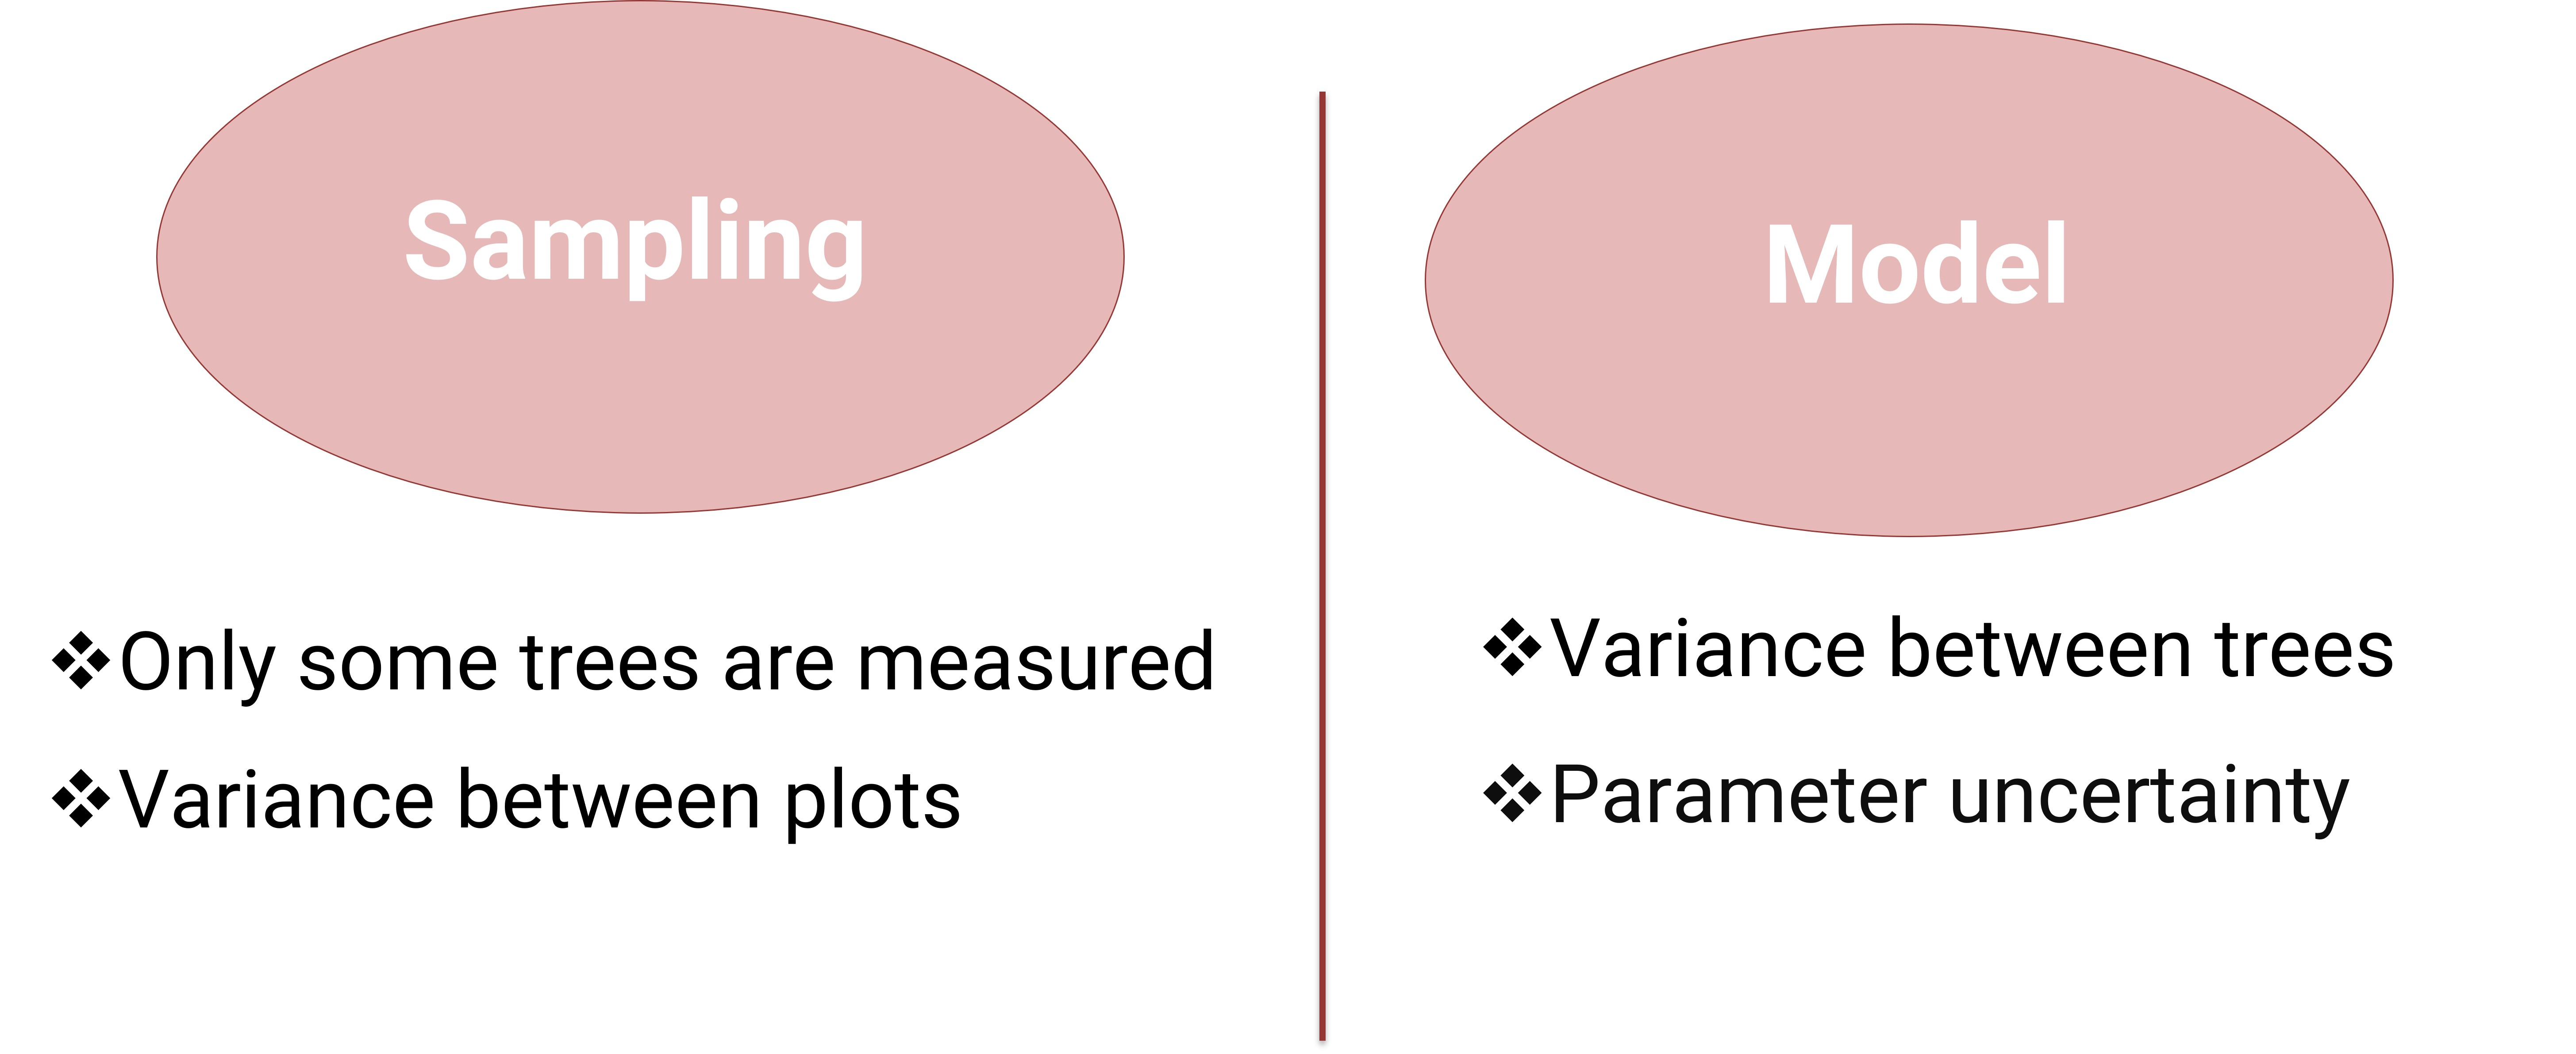
\includegraphics[width = 10cm, height = 4cm]{pic/Imagem8.jpg}
        \end{figure}  
\end{frame}

\begin{frame}{Uncertainty Sources}
\begin{itemize}
    \item Sampling
    \item Model
\end{itemize}
\begin{figure}
        \centering
        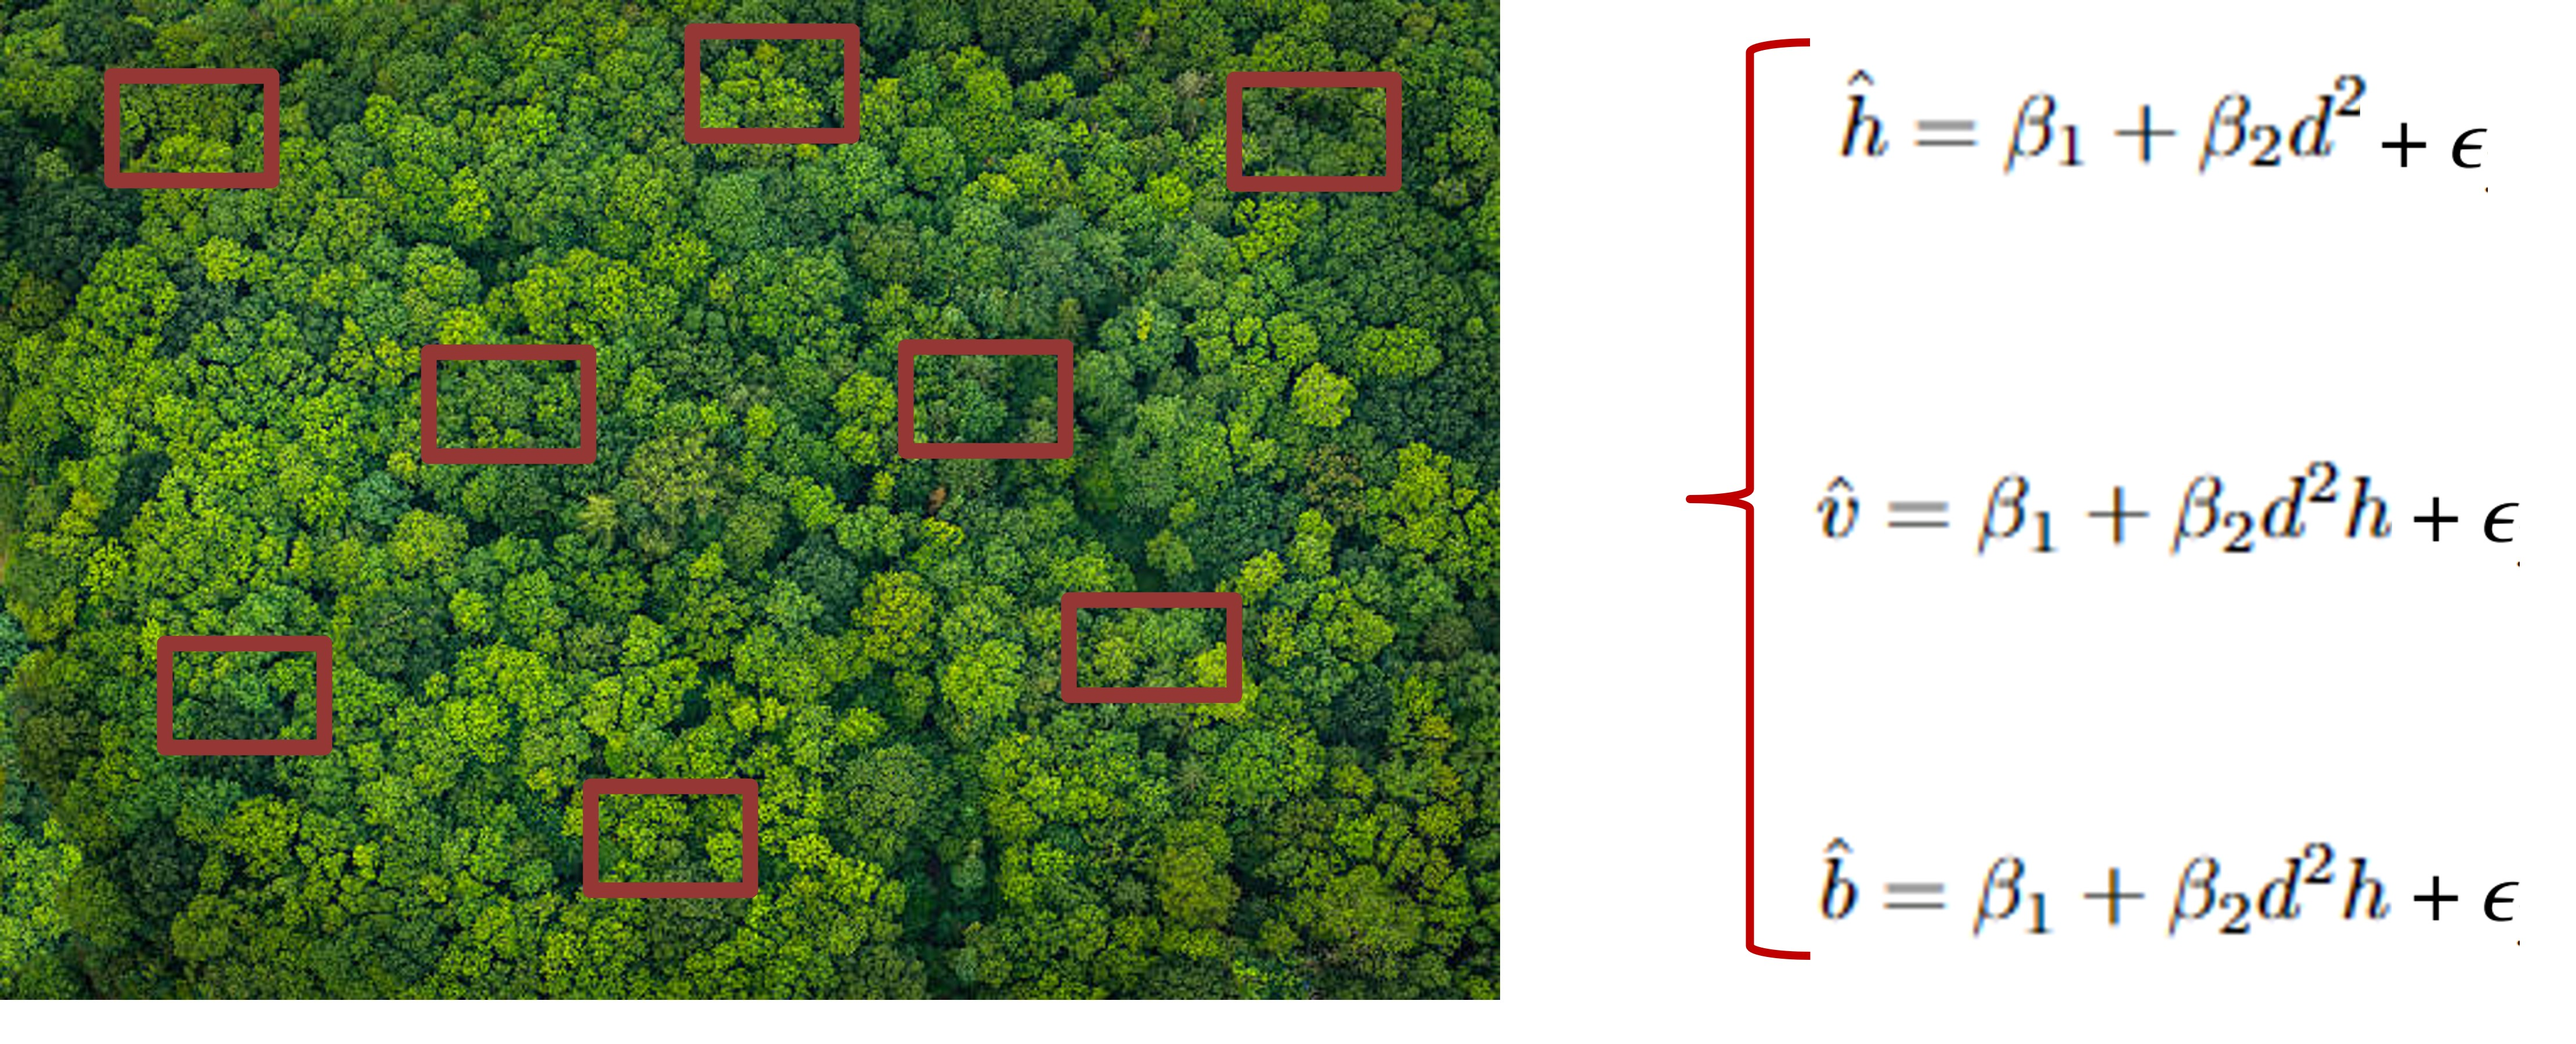
\includegraphics[width = 10cm, height = 4cm]{pic/primeirodia.jpg}
        \end{figure} 
\begin{itemize}
    \item Mean predictions for the forest.
    \item Production quantification: $volume (m^3), biomass (kg)$
\end{itemize}
\end{frame}

\begin{frame} {Uncertainty Sources} 
\begin{itemize}
    \item Model
\end{itemize}
\begin{figure}
        \centering
        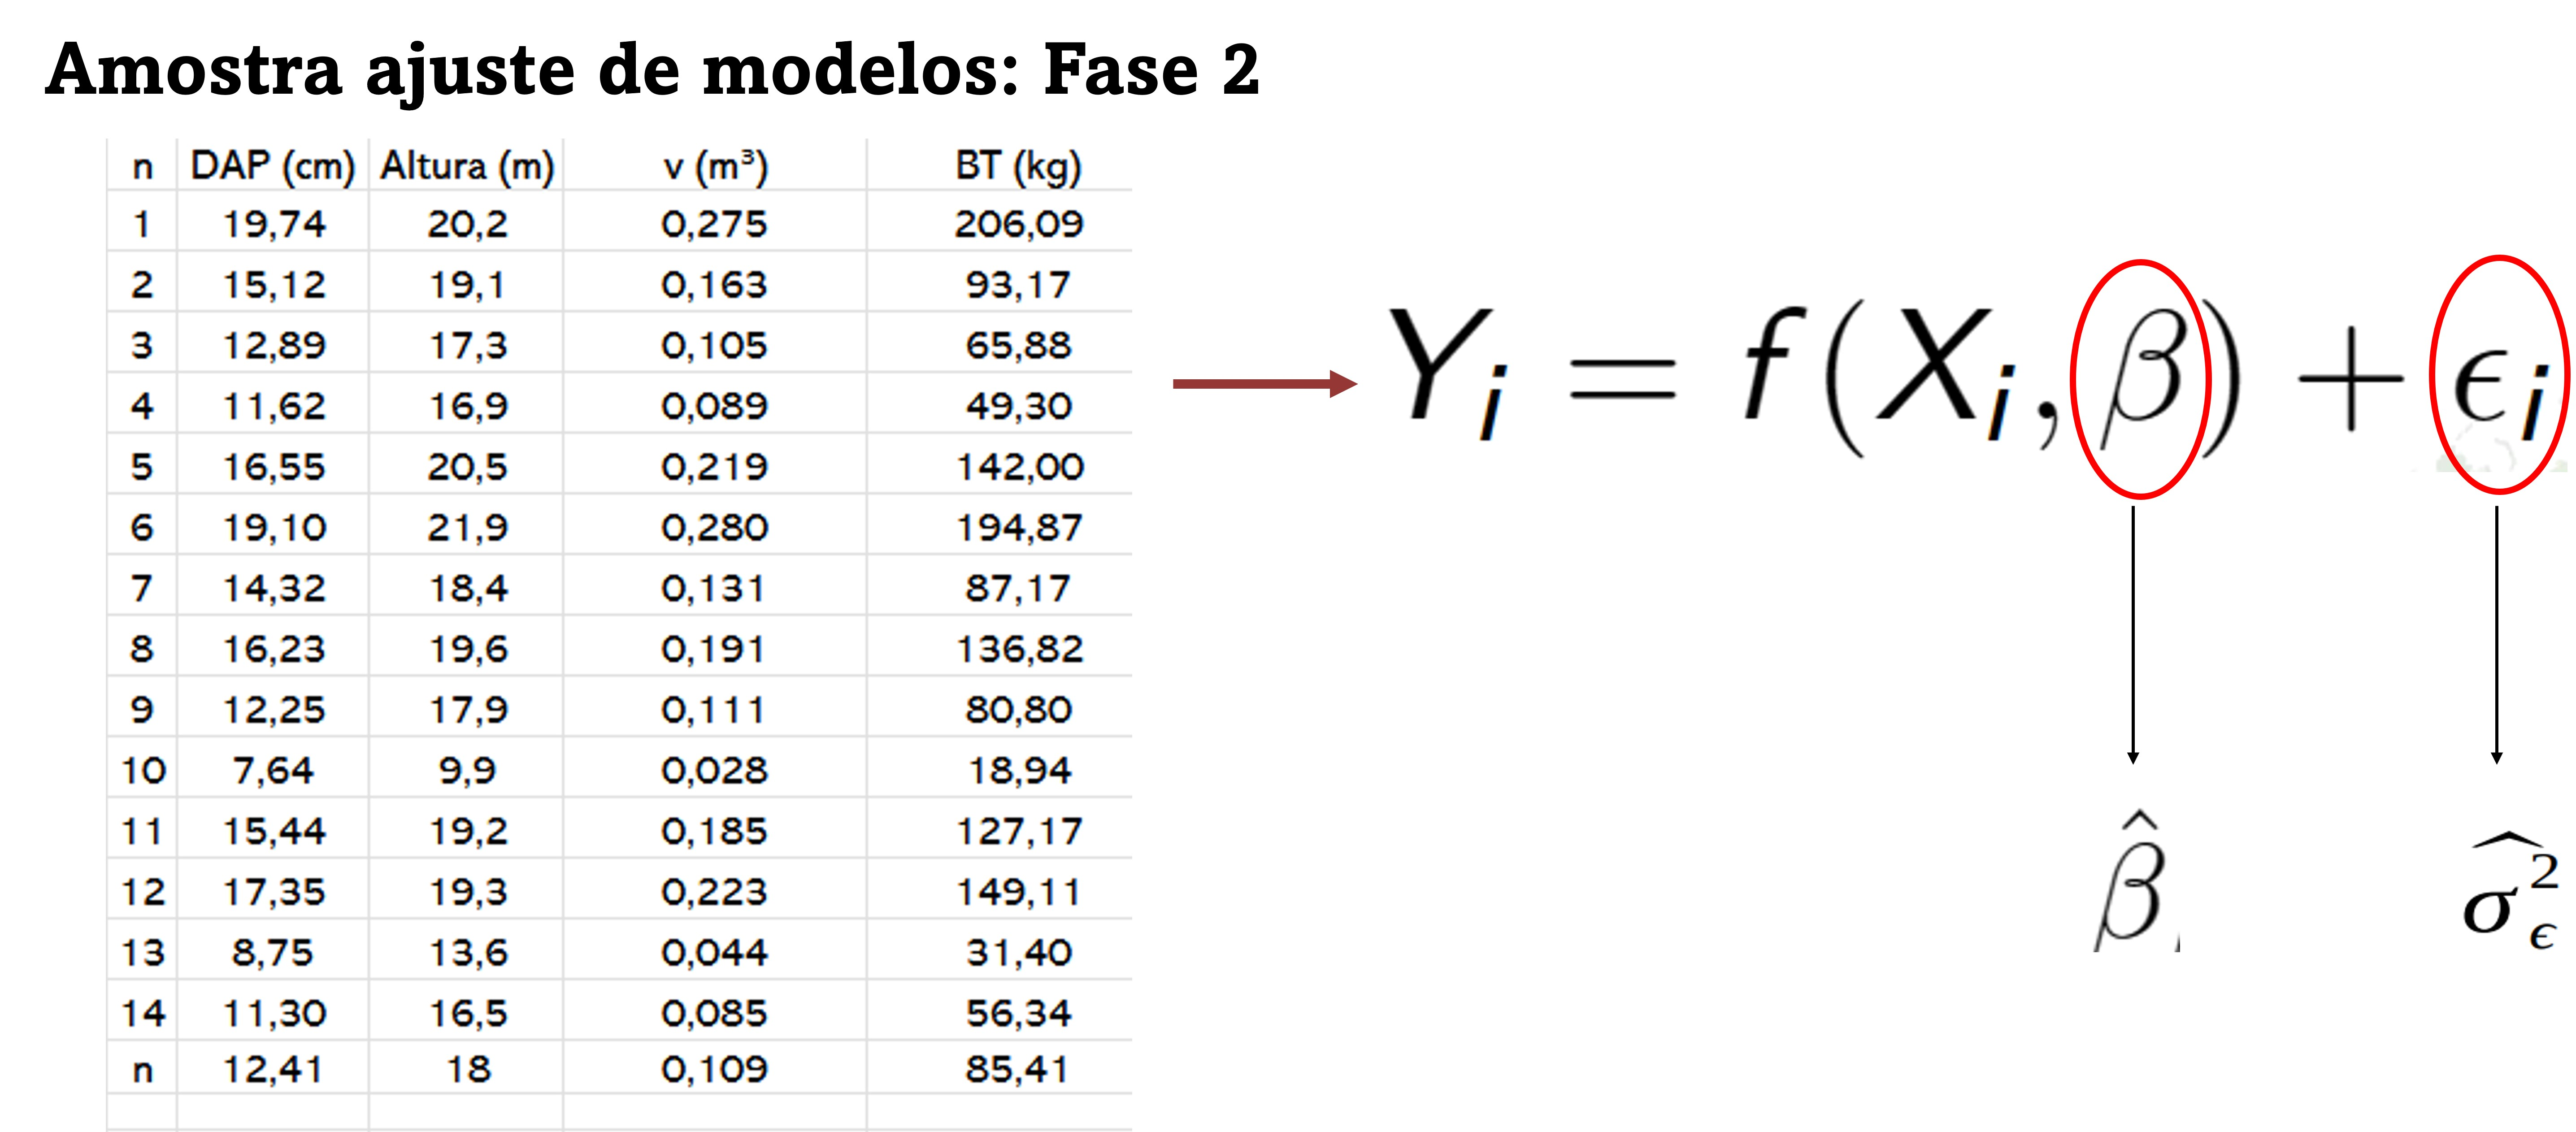
\includegraphics[width = 10cm, height = 4.5cm]{pic/sumodel.jpg}
        \end{figure} 
\end{frame}

\begin{frame} {Uncertainty Sources} 
\begin{itemize}
    \item Model
\end{itemize}
\begin{figure}
        \centering
        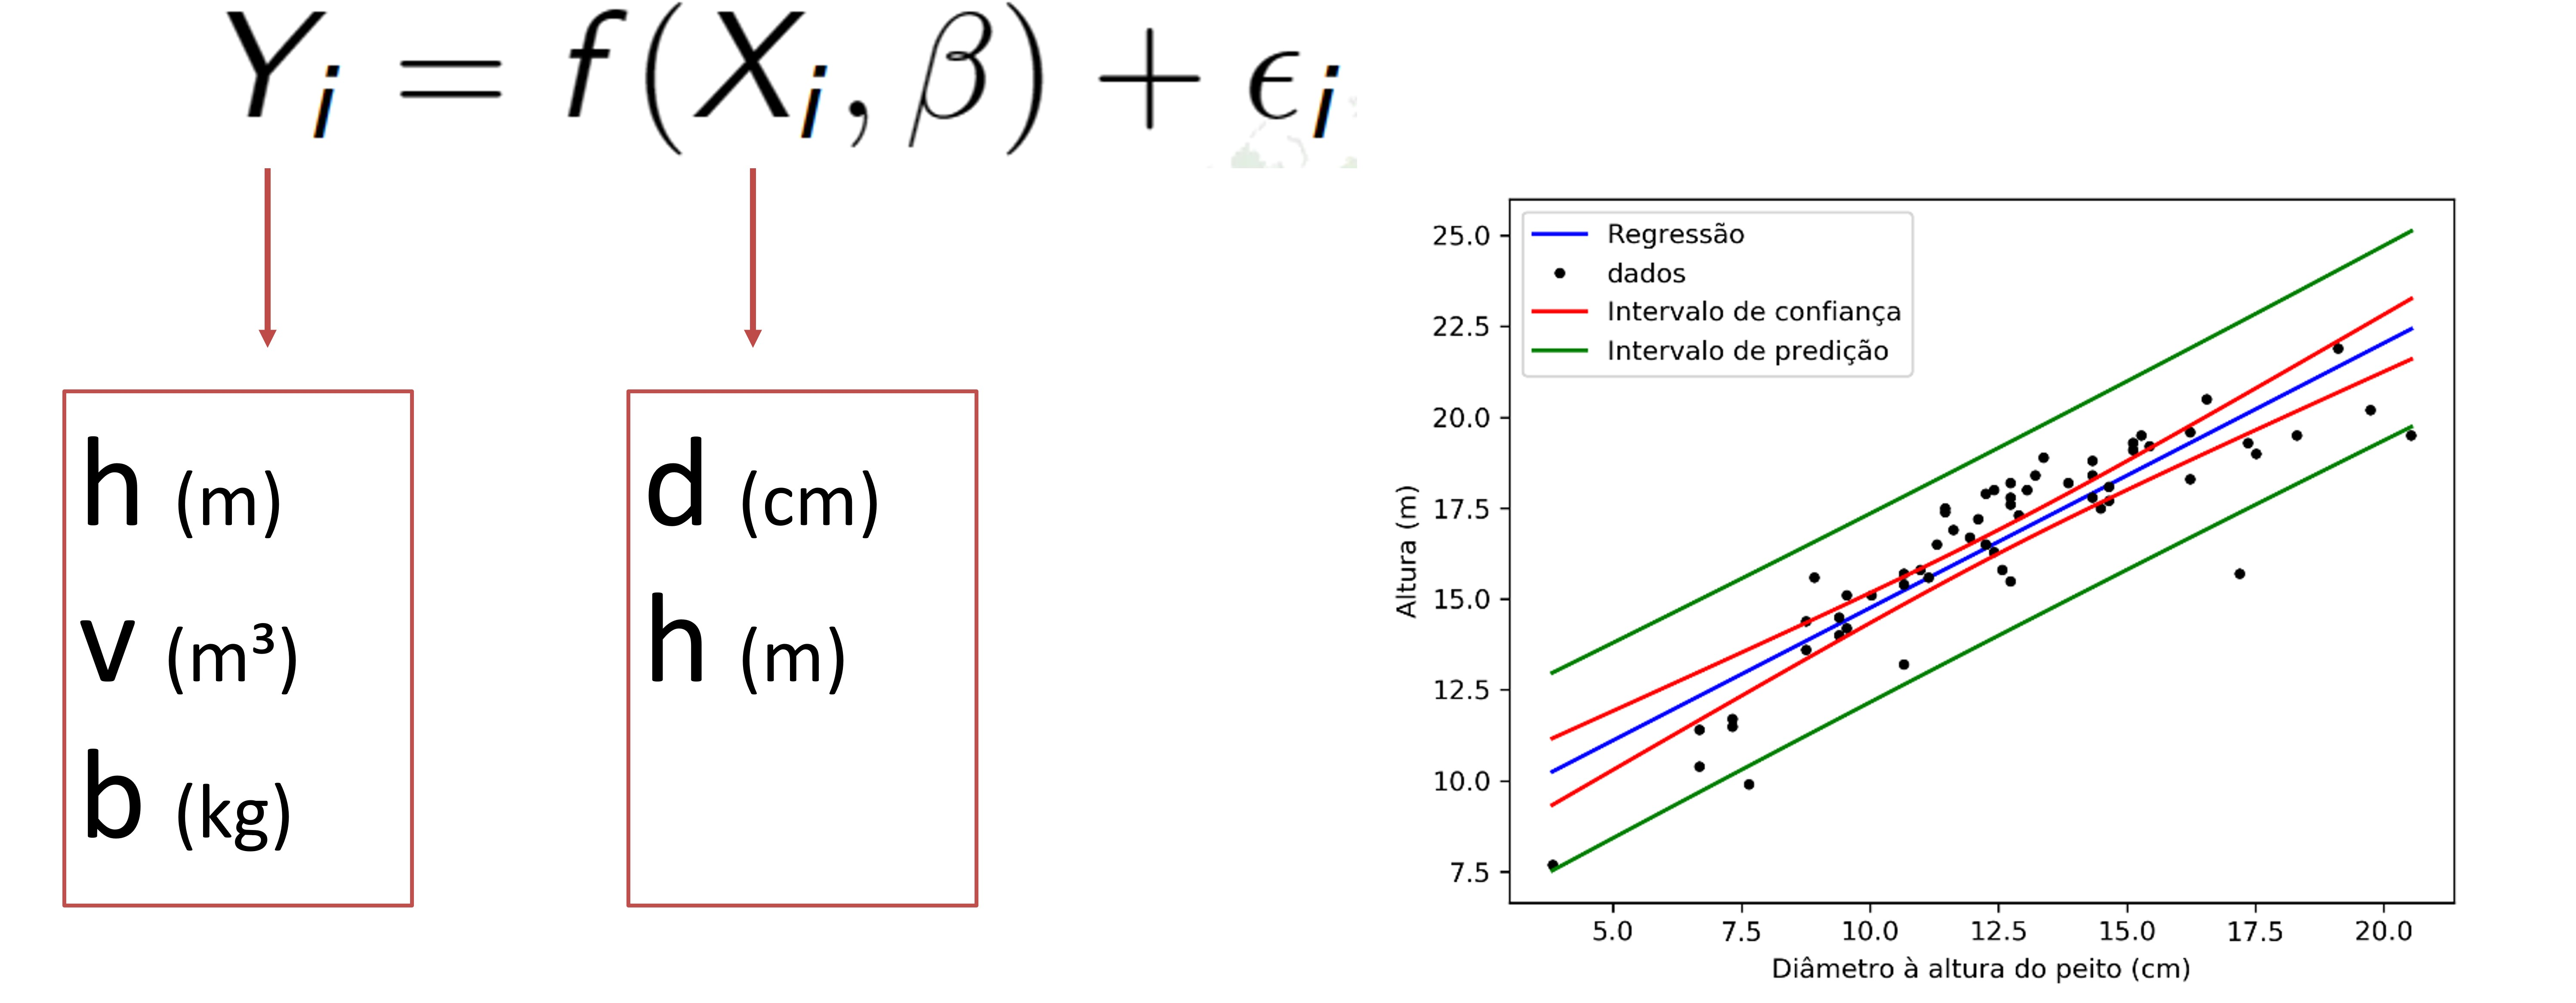
\includegraphics[width = 12cm, height = 4.5cm]{pic/suncertainty1.jpg}
        \end{figure} 
\end{frame}

\begin{frame} {Uncertainty Sources} 
\begin{itemize}
    \item Model
    \end{itemize}
\begin{figure}
        \centering
        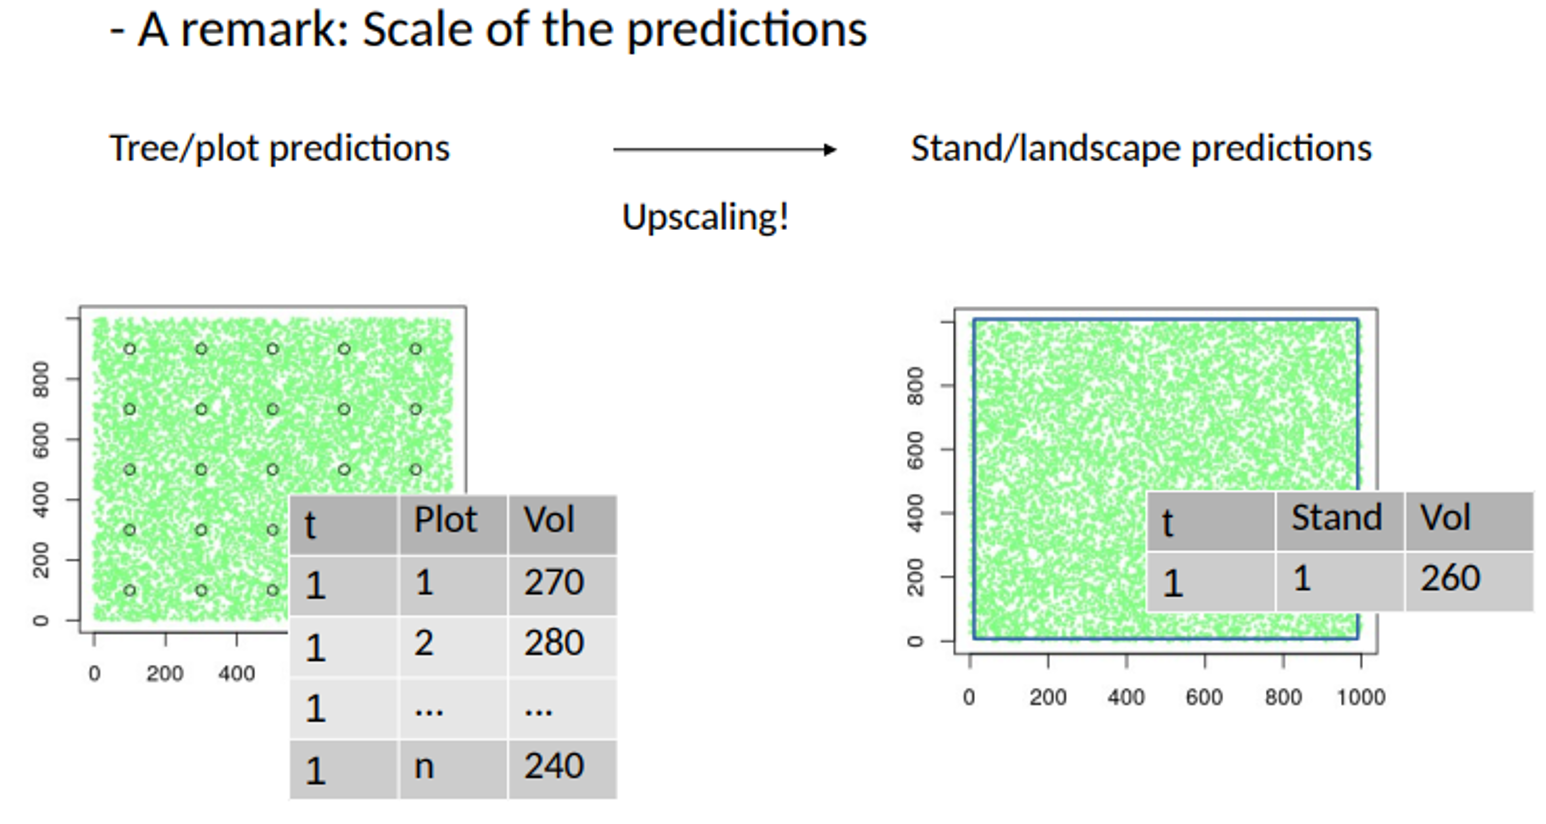
\includegraphics[width = 11cm, height = 6cm]{pic/sources.png}
        \end{figure} 
\end{frame}

\begin{frame} {Uncertainty Sources} 
\begin{figure}
        \centering
        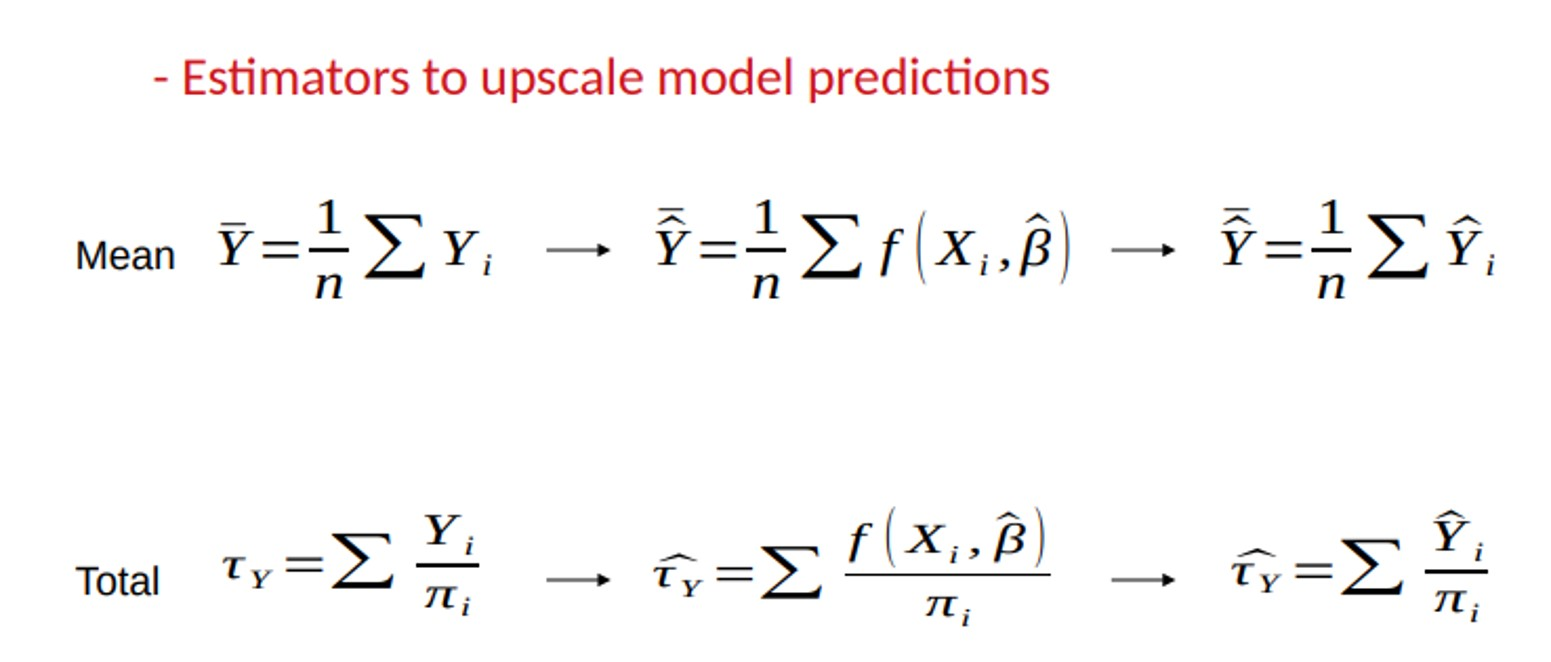
\includegraphics[width = 11cm, height = 6cm]{pic/meanandtotal.jpg}
        \end{figure} 
\end{frame}


\begin{frame} {Uncertainty Sources} 
\begin{itemize}
    \item Sampling
    \end{itemize}
\begin{figure}
        \centering
        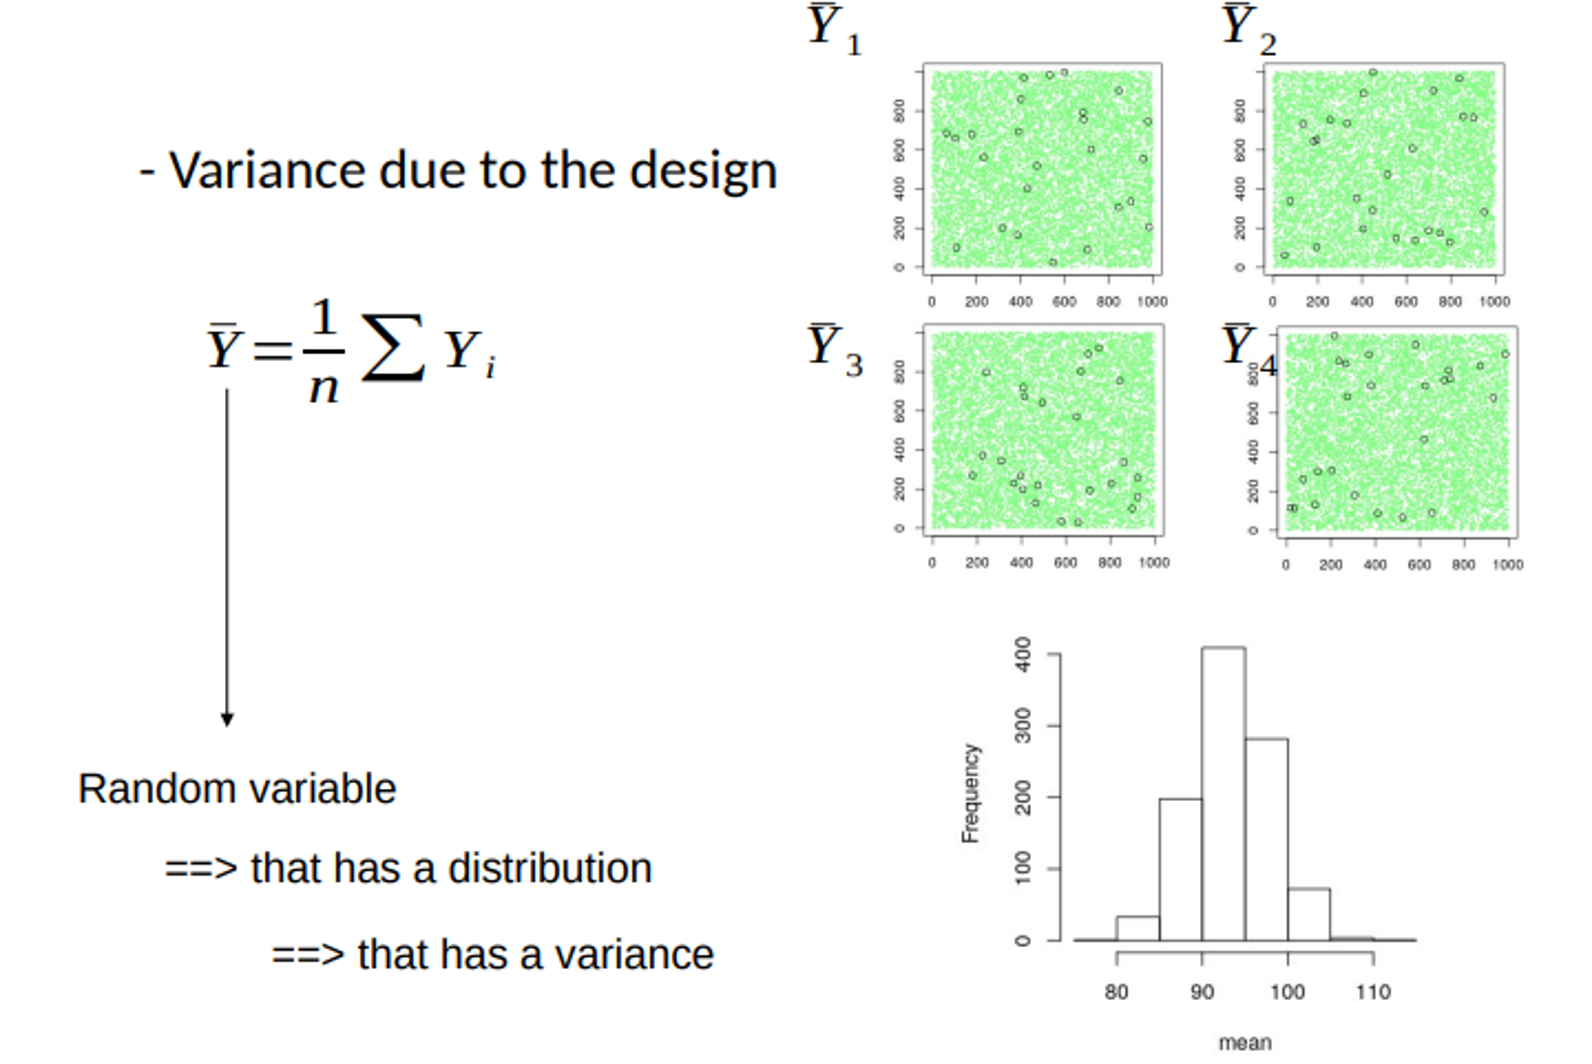
\includegraphics[width = 11cm, height = 6cm]{pic/varinv.png}
        \end{figure} 
\end{frame}

\begin{frame} {Uncertainty Sources} 
\begin{itemize}
    \item What metric do we use to measure uncertainty?
    \end{itemize}
\end{frame}

\begin{frame} {Uncertainty Sources} 
\begin{figure}
        \centering
        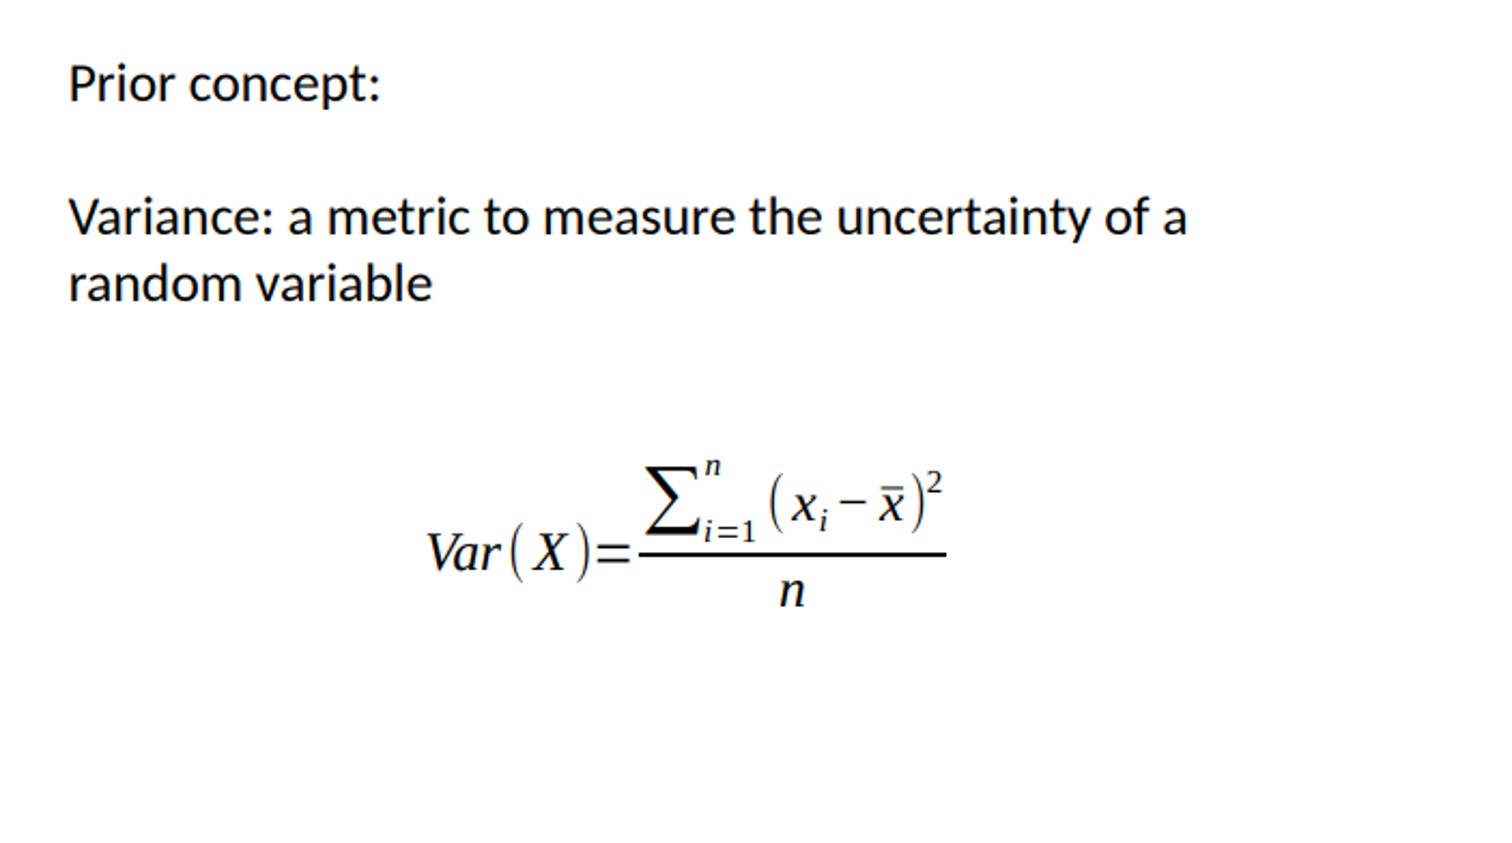
\includegraphics[width = 11cm, height = 7.5cm]{pic/variancia.jpg}
        \end{figure} 
\end{frame}

\begin{frame} {Uncertainty Sources} 
\begin{figure}
        \centering
        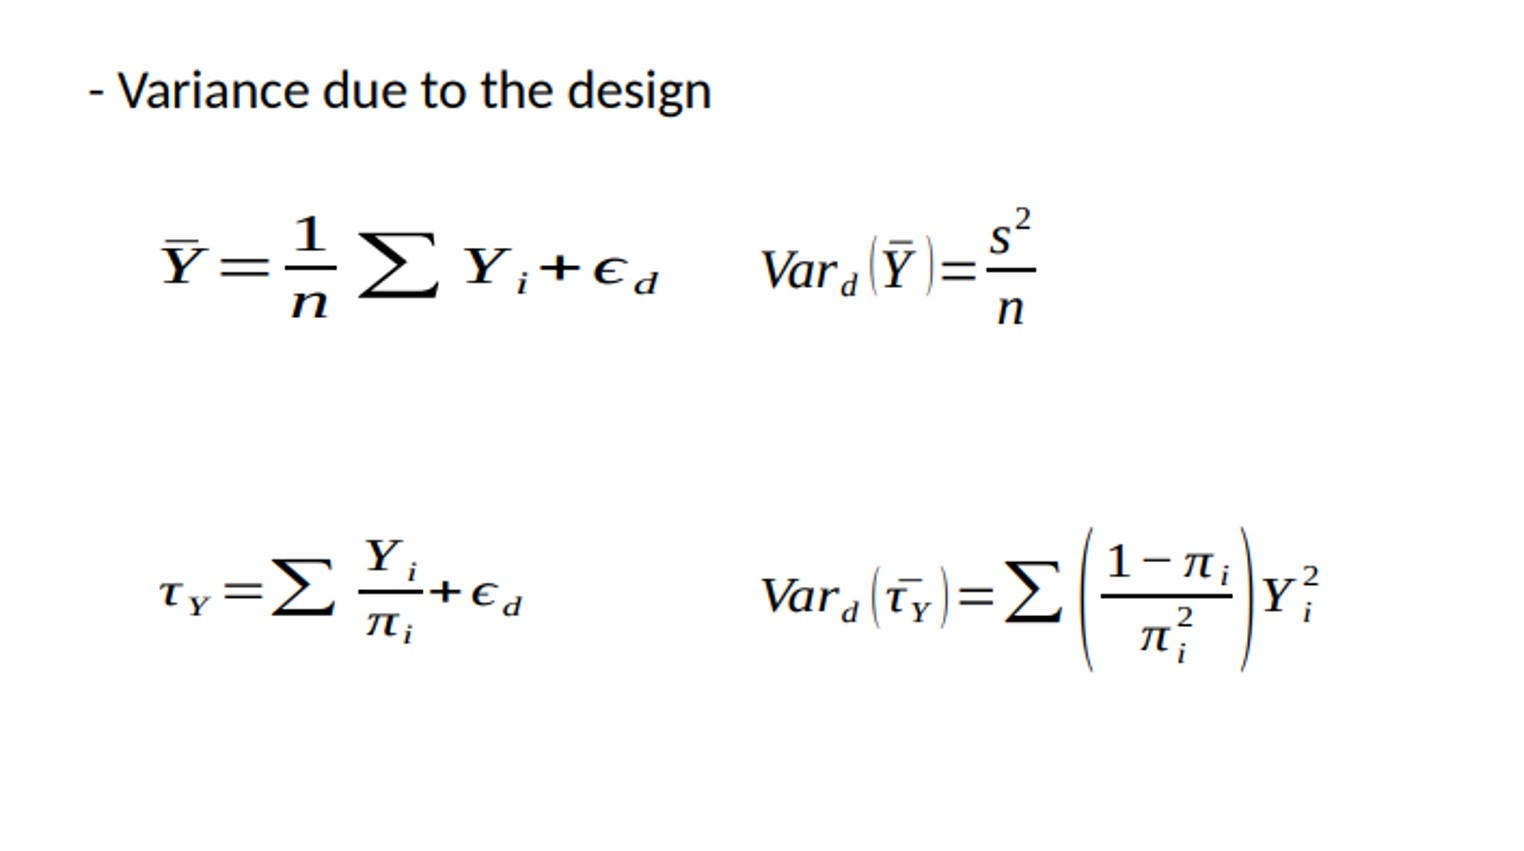
\includegraphics[width = 11cm, height = 6cm]{pic/variduedesign.jpg}
        \end{figure} 
\end{frame}

\begin{frame} {Uncertainty Sources} 
\begin{figure}
        \centering
        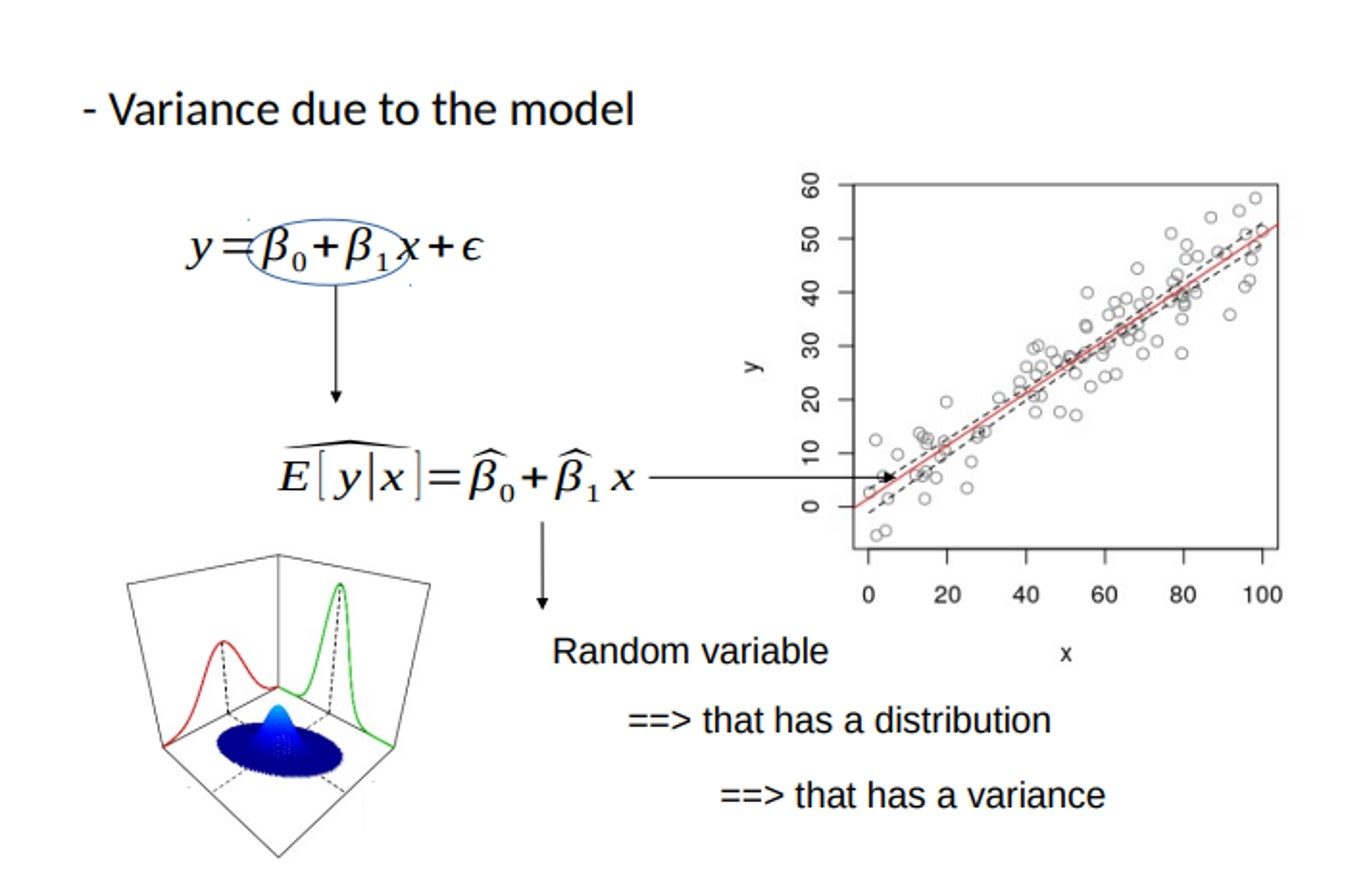
\includegraphics[width = 11cm, height = 6cm]{pic/duemodel.jpg}
        \end{figure} 
\end{frame}

\begin{frame} {Uncertainty Sources} 
\begin{figure}
        \centering
        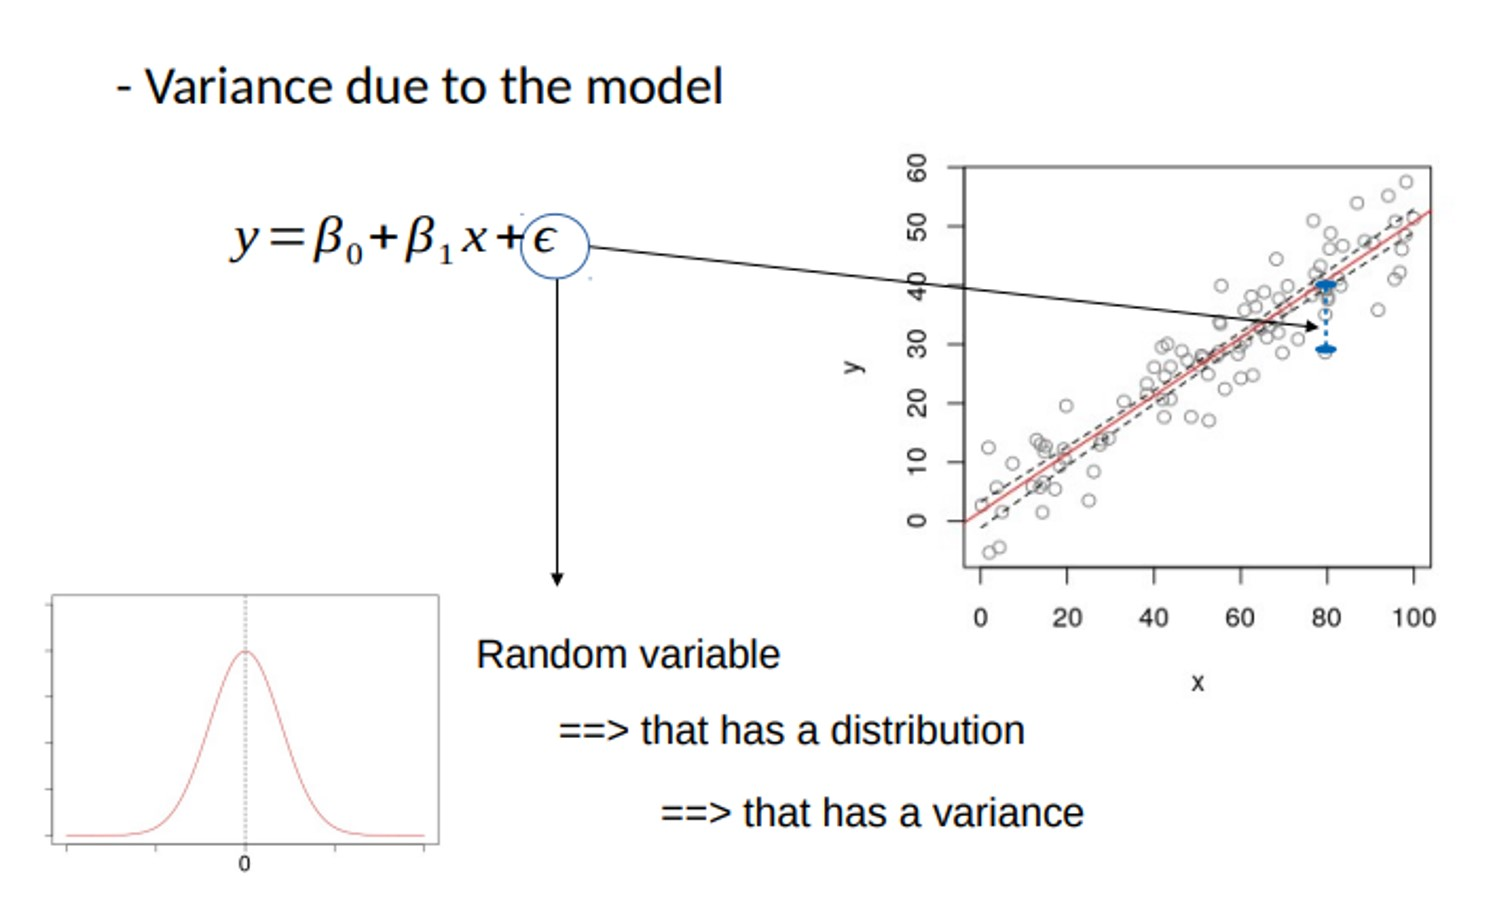
\includegraphics[width = 11cm, height = 6cm]{pic/duethemodel.jpg}
        \end{figure} 
\end{frame}

\begin{frame} {Uncertainty Sources} 
Uncertainty in the estimates 
\begin{figure}
        \centering
        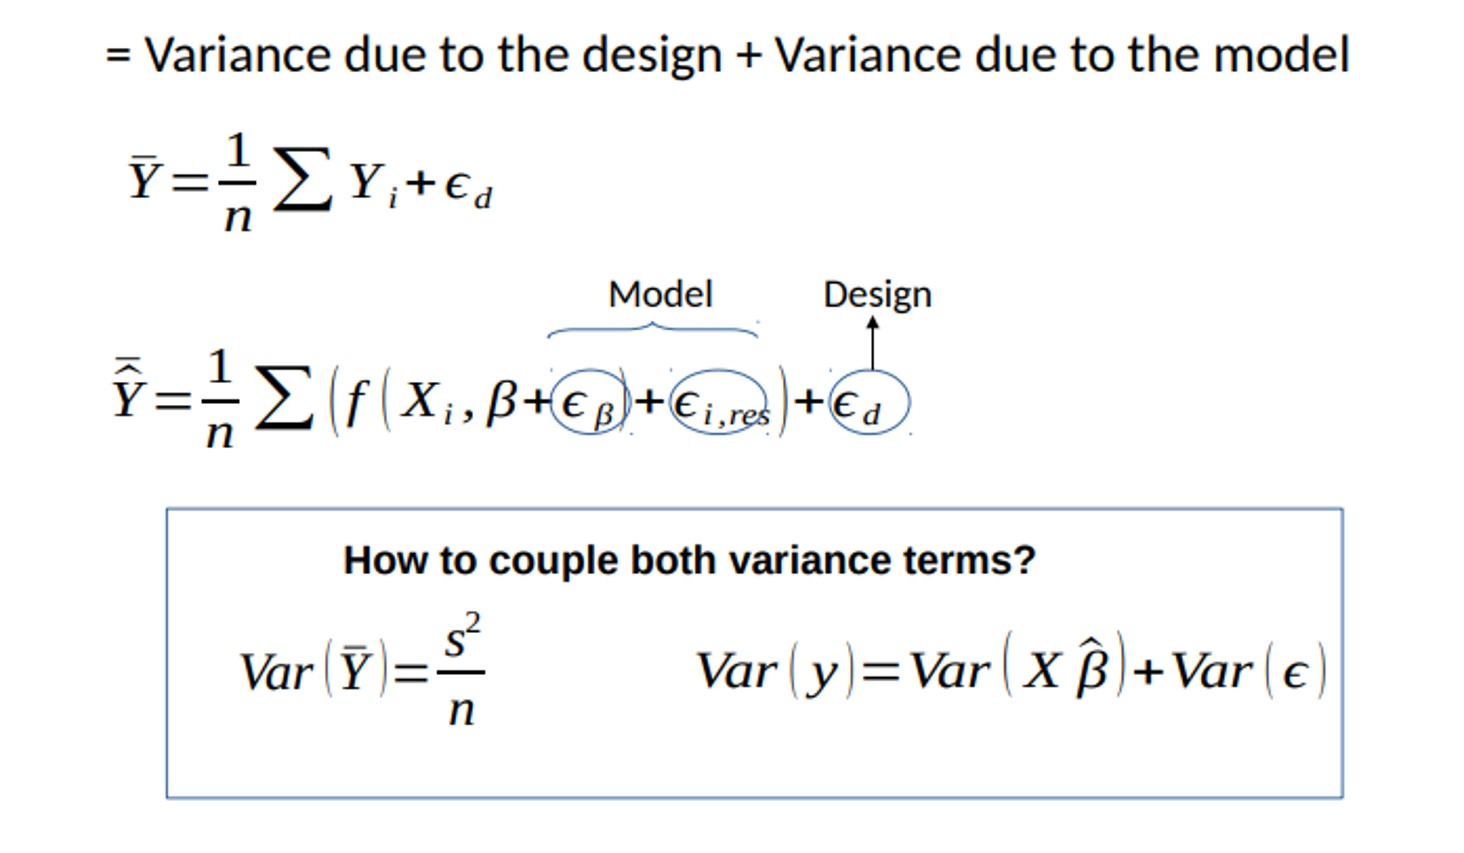
\includegraphics[width = 11cm, height = 6cm]{pic/modelinv.jpg}
        \end{figure} 
\end{frame}

\section{Methods}
\begin{frame}{Quantifying the uncertainty}
Hybrid variance estimators
\begin{itemize}
    \item Analytics
    \item Computacional - Bootstrap, MC 
\end{itemize}

\begin{figure}
        \centering
        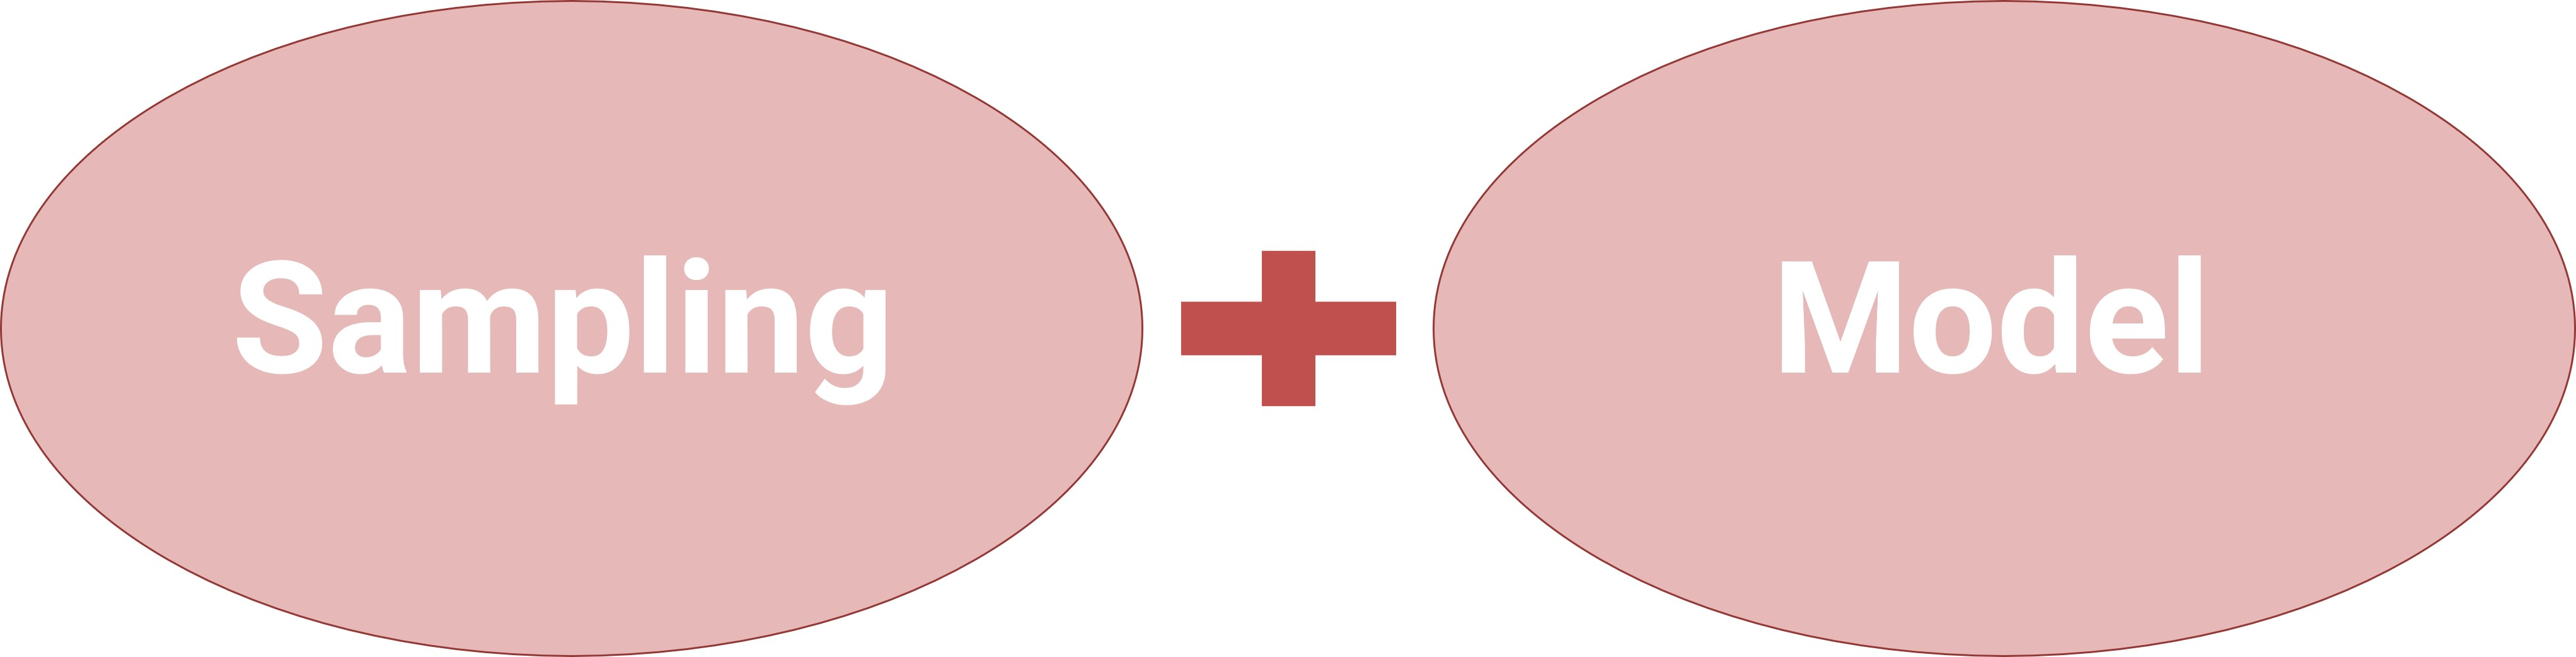
\includegraphics[width = 10cm, height = 3cm]{pic/fontes.jpg}
        \end{figure}  
    
\end{frame}

\begin{frame}{Quantifying the uncertainty}
\begin{figure}
        \centering
        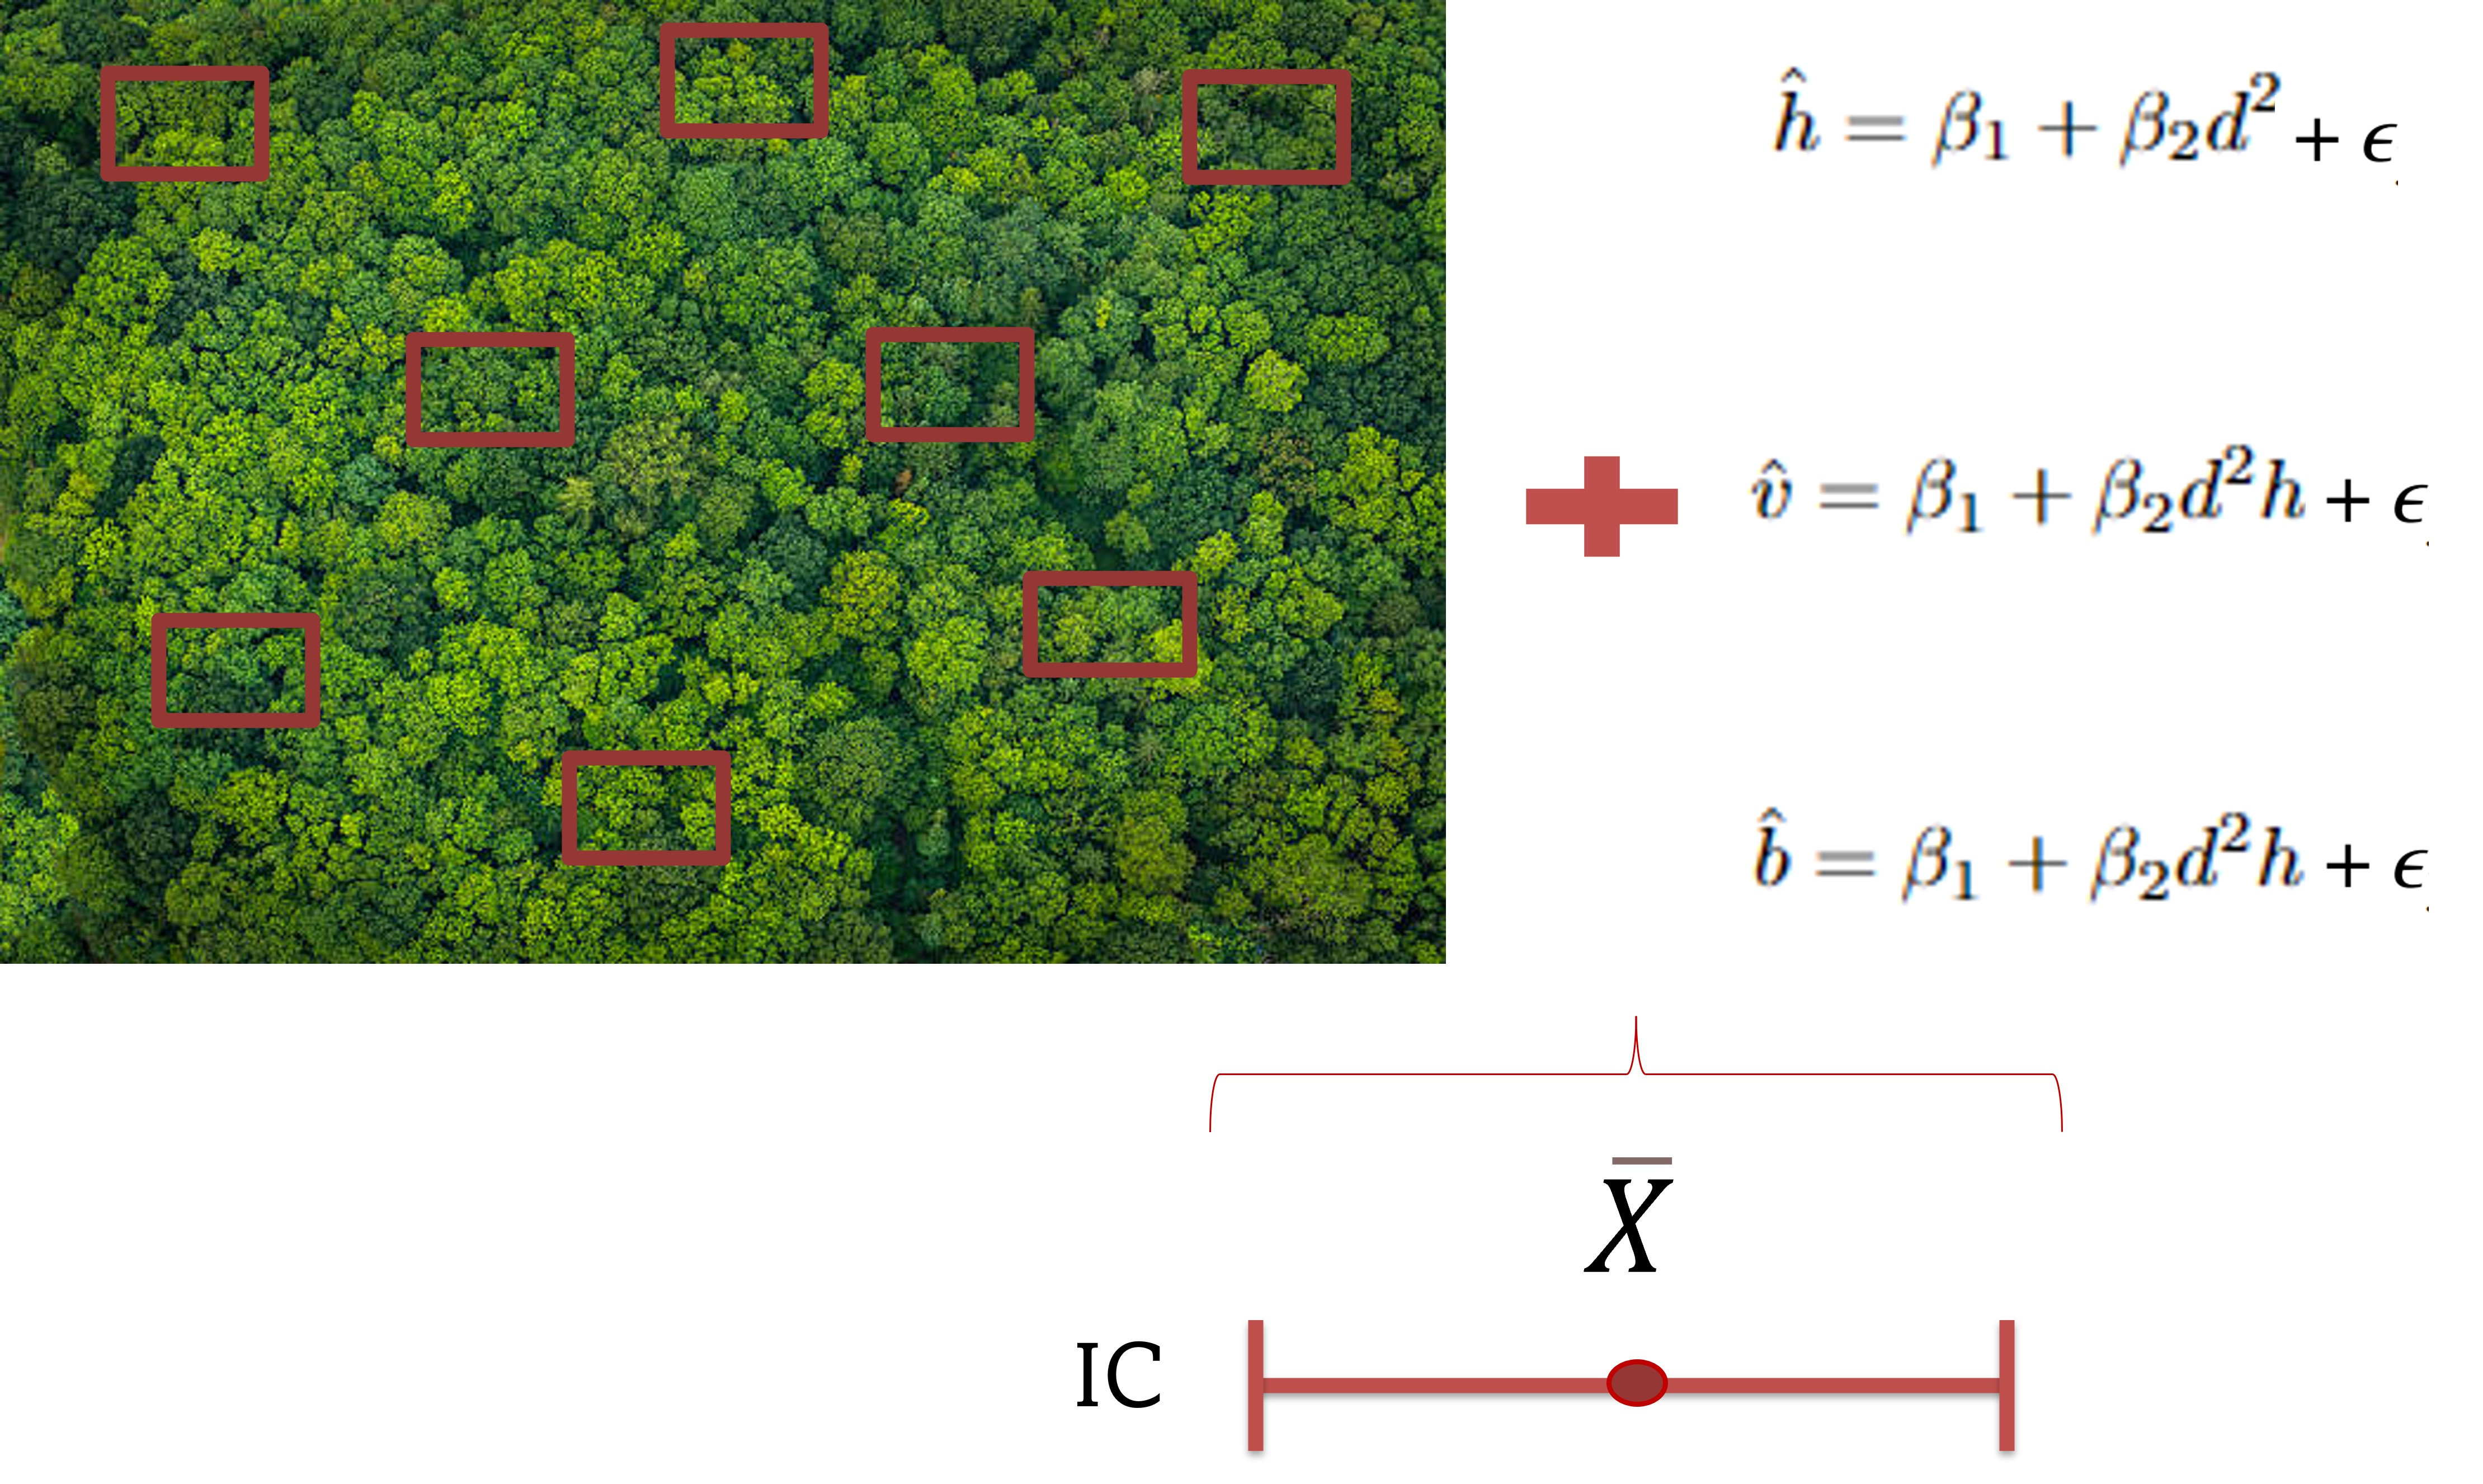
\includegraphics[width = 10cm, height = 5.5cm]{pic/fontes2.jpg}
        \end{figure}          
\end{frame}


\begin{frame}{Quantifying the uncertainty}
Analytic
\begin{itemize}
    \item Mathematical treatment of algebraic form
    \item Obtain the variance value for each tree 
\end{itemize}

\begin{figure}
        \centering
        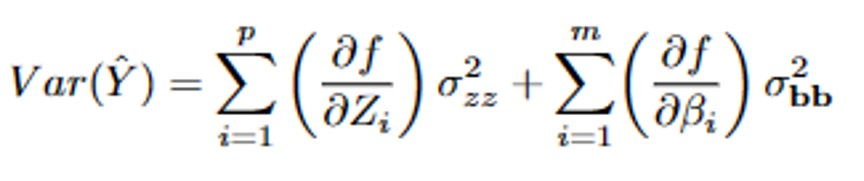
\includegraphics[width = 8cm, height = 1.5cm]{pic/analitico1.jpg}
        \end{figure}  
    
\end{frame}


\begin{frame}{Quantifying the uncertainty}
Analytic
\begin{itemize}
    \item Linear model
\end{itemize}

\begin{figure}
        \centering
        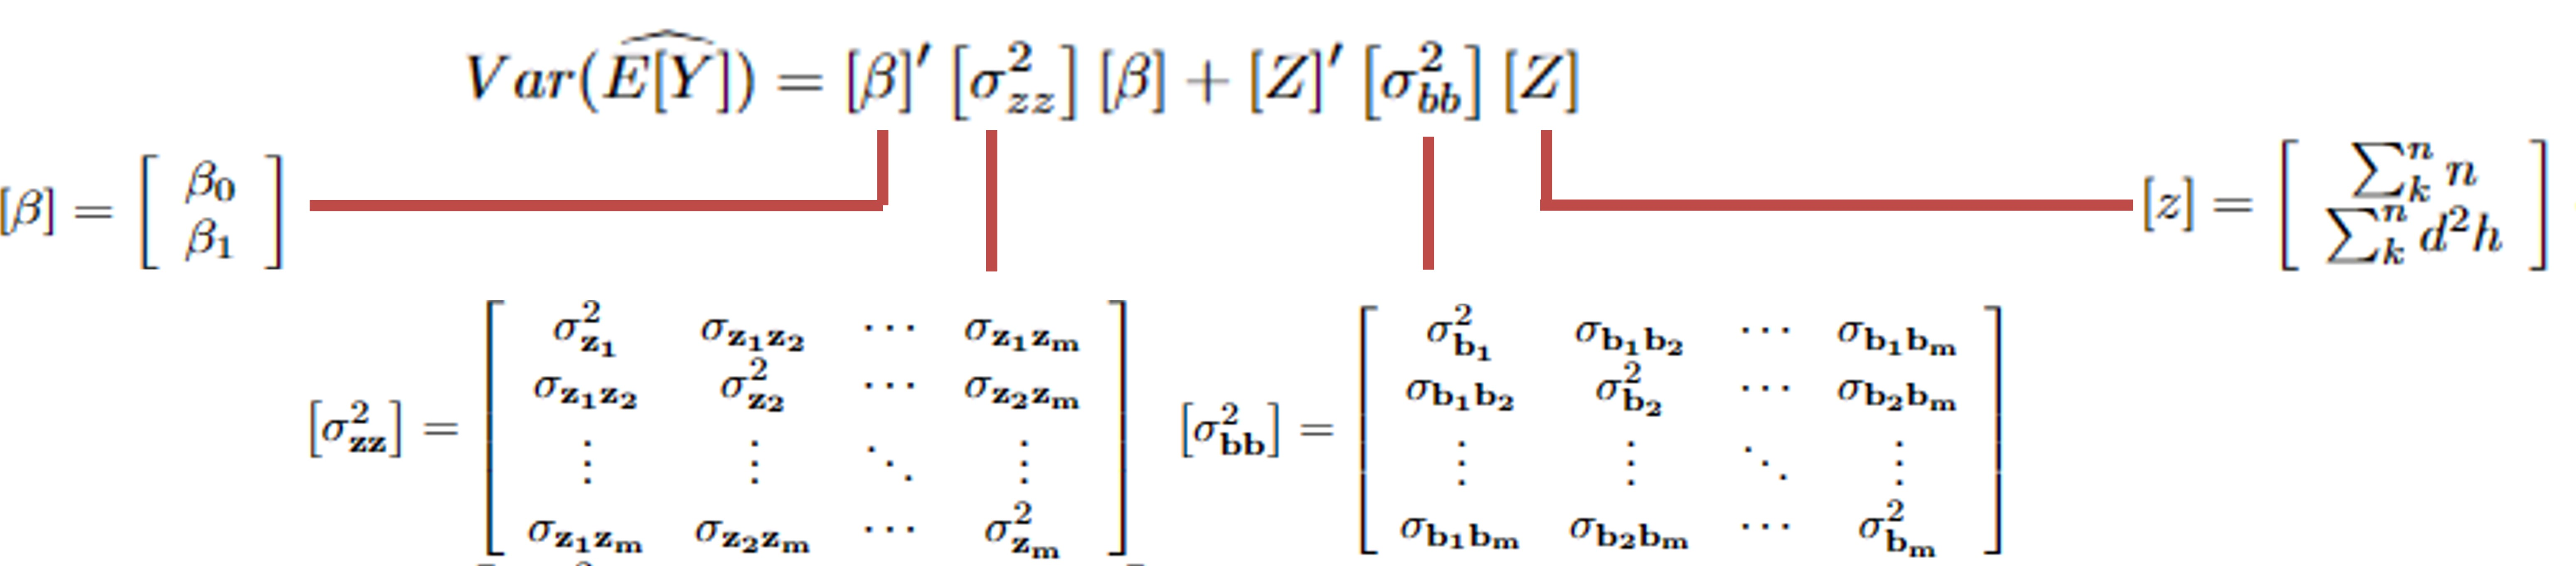
\includegraphics[width = 10cm, height = 3cm]{pic/analitico.jpg}
        \end{figure}  
    
\end{frame}

\begin{frame}{Quantifying the uncertainty}
Analytic
\begin{itemize}
    \item Nonlinear model
\end{itemize}

\begin{figure}
        \centering
        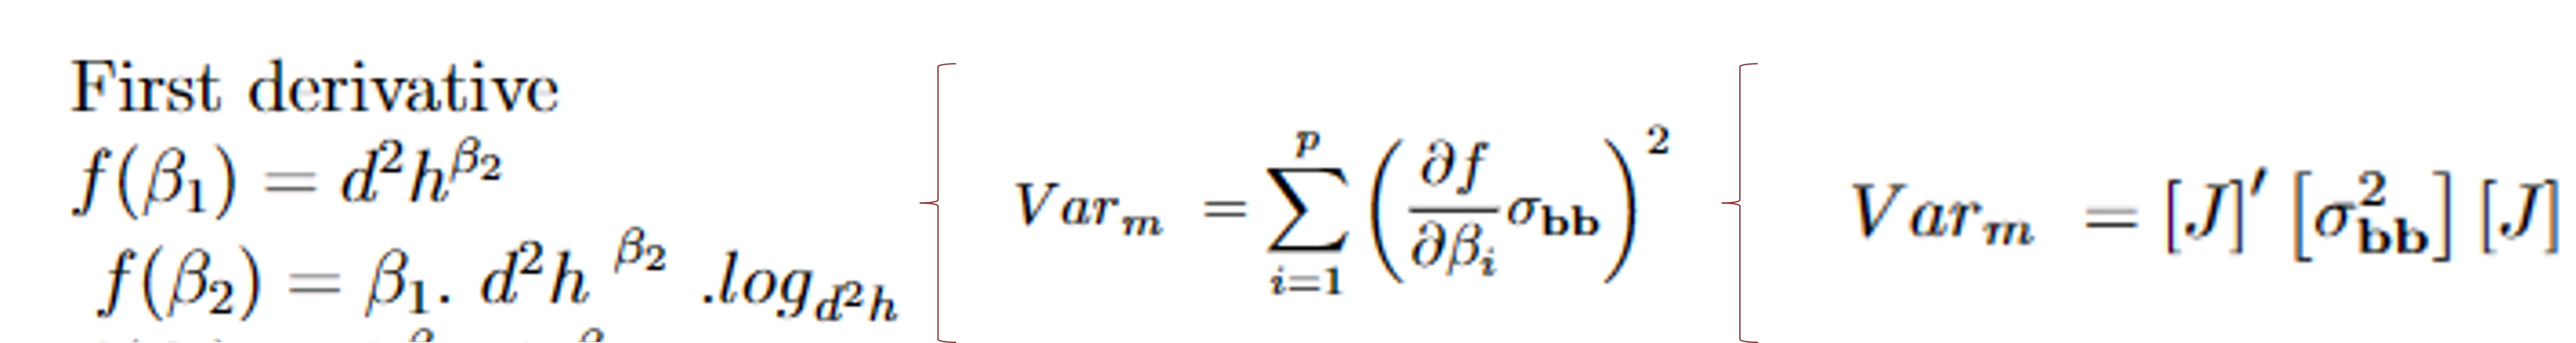
\includegraphics[width = 10cm, height = 1.5cm]{pic/Imagem3.jpg}
        \end{figure}  
    
\end{frame}

\begin{frame}{Quantifying the uncertainty}
Computational - Bootstrap
\begin{itemize}
    \item Requires more computing resources
    \item Large number of simulations of random variables in order to reproduce the variability of a process
    \item Recreation of the variability of a complex process through resampling 
\end{itemize}

\begin{figure}
        \centering
        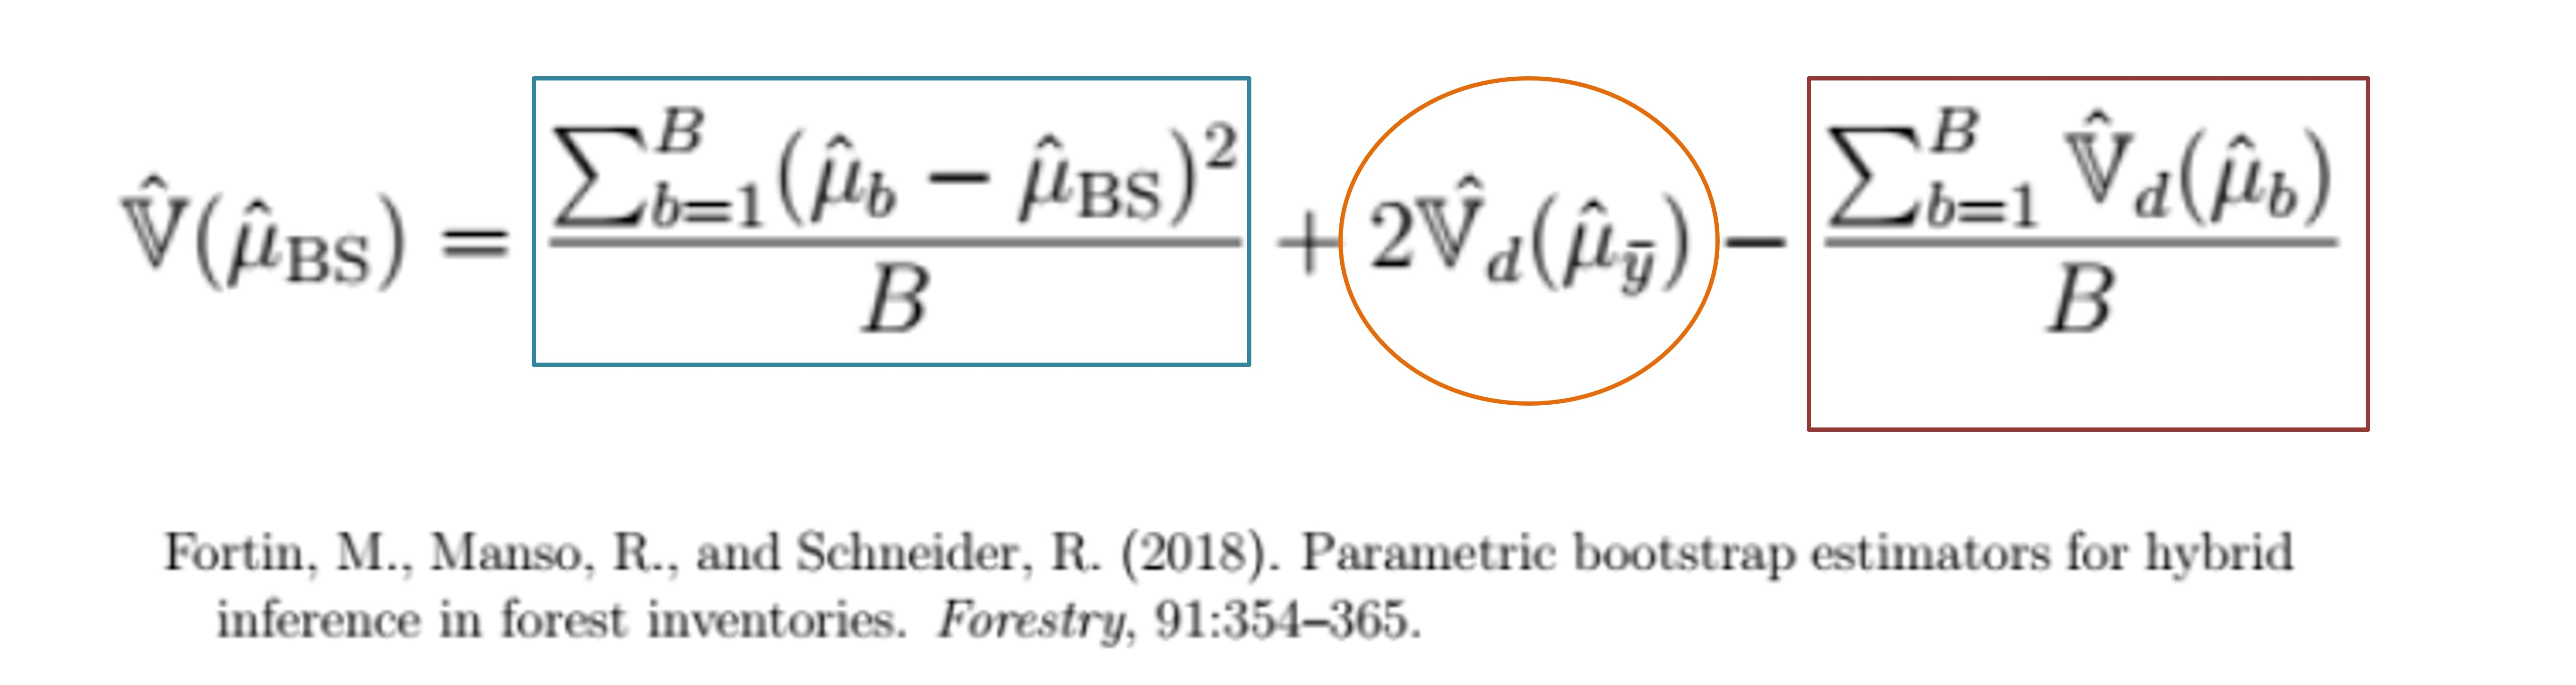
\includegraphics[width = 10cm, height = 2cm]{pic/bootstrap.jpg}
        \end{figure}      
\end{frame}

\begin{frame}{Quantifying the uncertainty}
Computational - Bootstrap
\begin{figure}
        \centering
        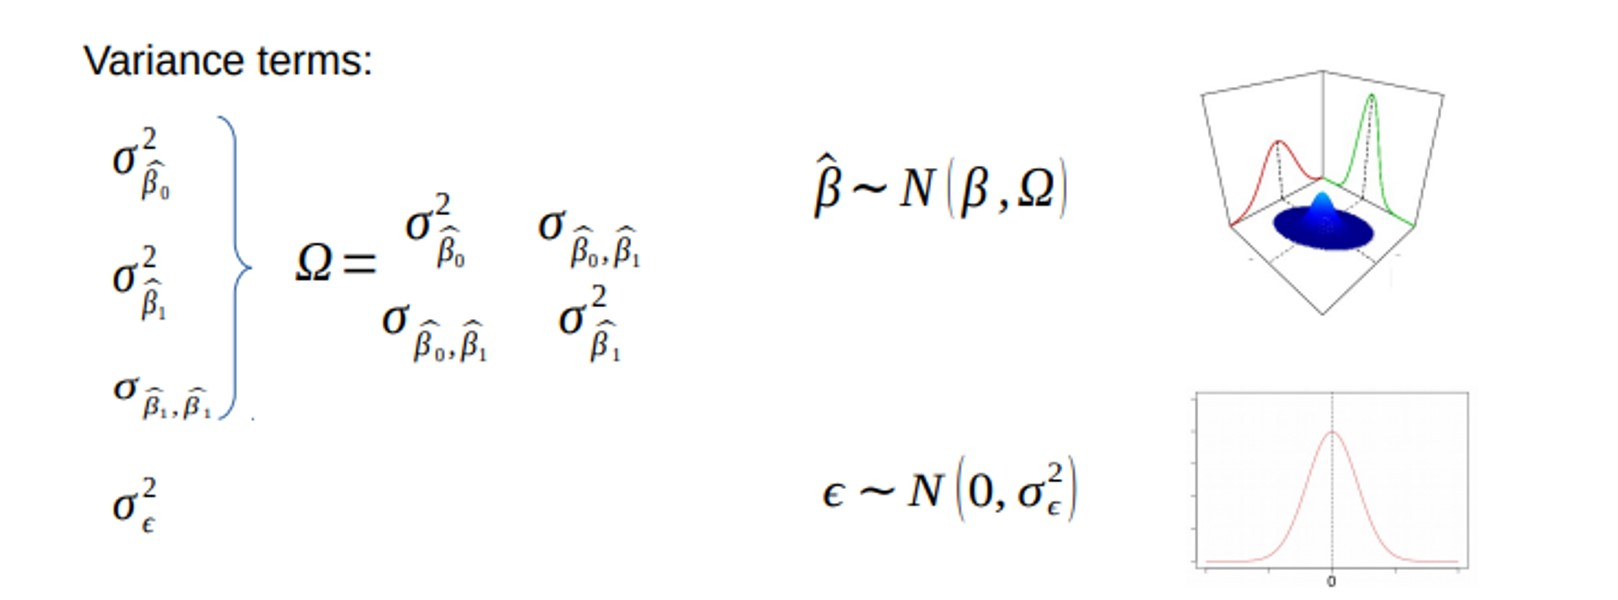
\includegraphics[width = 10cm, height = 4cm]{pic/bootstrap1.jpg}
        \end{figure}      
\end{frame}

\begin{frame}{Quantifying the uncertainty}
Computational - Bootstrap
\begin{figure}
        \centering
        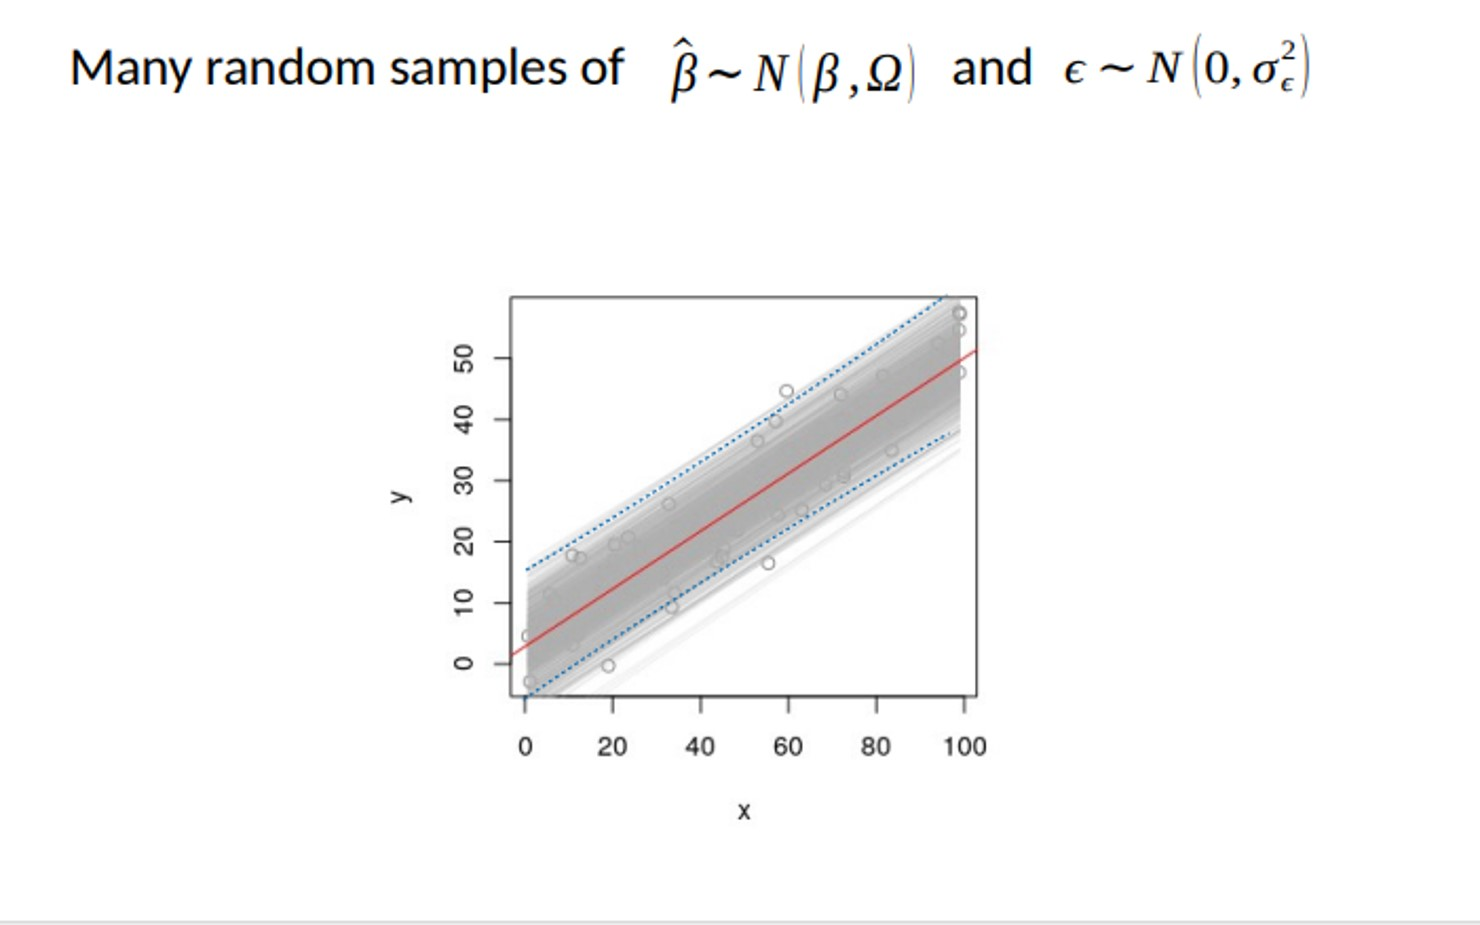
\includegraphics[width = 10cm, height = 5cm]{pic/bootstrap2.jpg}
        \end{figure}      
\end{frame}

\section{Practical Exercice}
\begin{frame}{}
\begin{block}{What we will do?}
    \begin{itemize}
\item Processing and application of methods (BS)
\item Graphs - Results
    \end{itemize}
\end{block}
\begin{block}{What we will use?}
    \begin{itemize}
\item Rstudio
\item Biomass
\item Model: $\hat{y}=\beta_1+\beta_2 d^2h$ 
\item Database: Stands of \textit{Acacia mearnsii}
    \end{itemize}
\end{block}
\end{frame}


\begin{frame}
\begin{block}{Questions to answer}
       \begin{itemize}
           \item What influences model-related uncertainty?
             \begin{itemize}
           \item Evaluate the influence of the number of trees to fit the model.
       \end{itemize}
        \end{itemize}
\begin{itemize}
    \item What influences sampling-related uncertainty?
    \begin{itemize}
        \item Evaluate the influence of sampling size on the uncertainty.
    \end{itemize}
 \end{itemize}
\end{block} 
\end{frame}

\begin{frame}
\begin{figure}
        \centering
        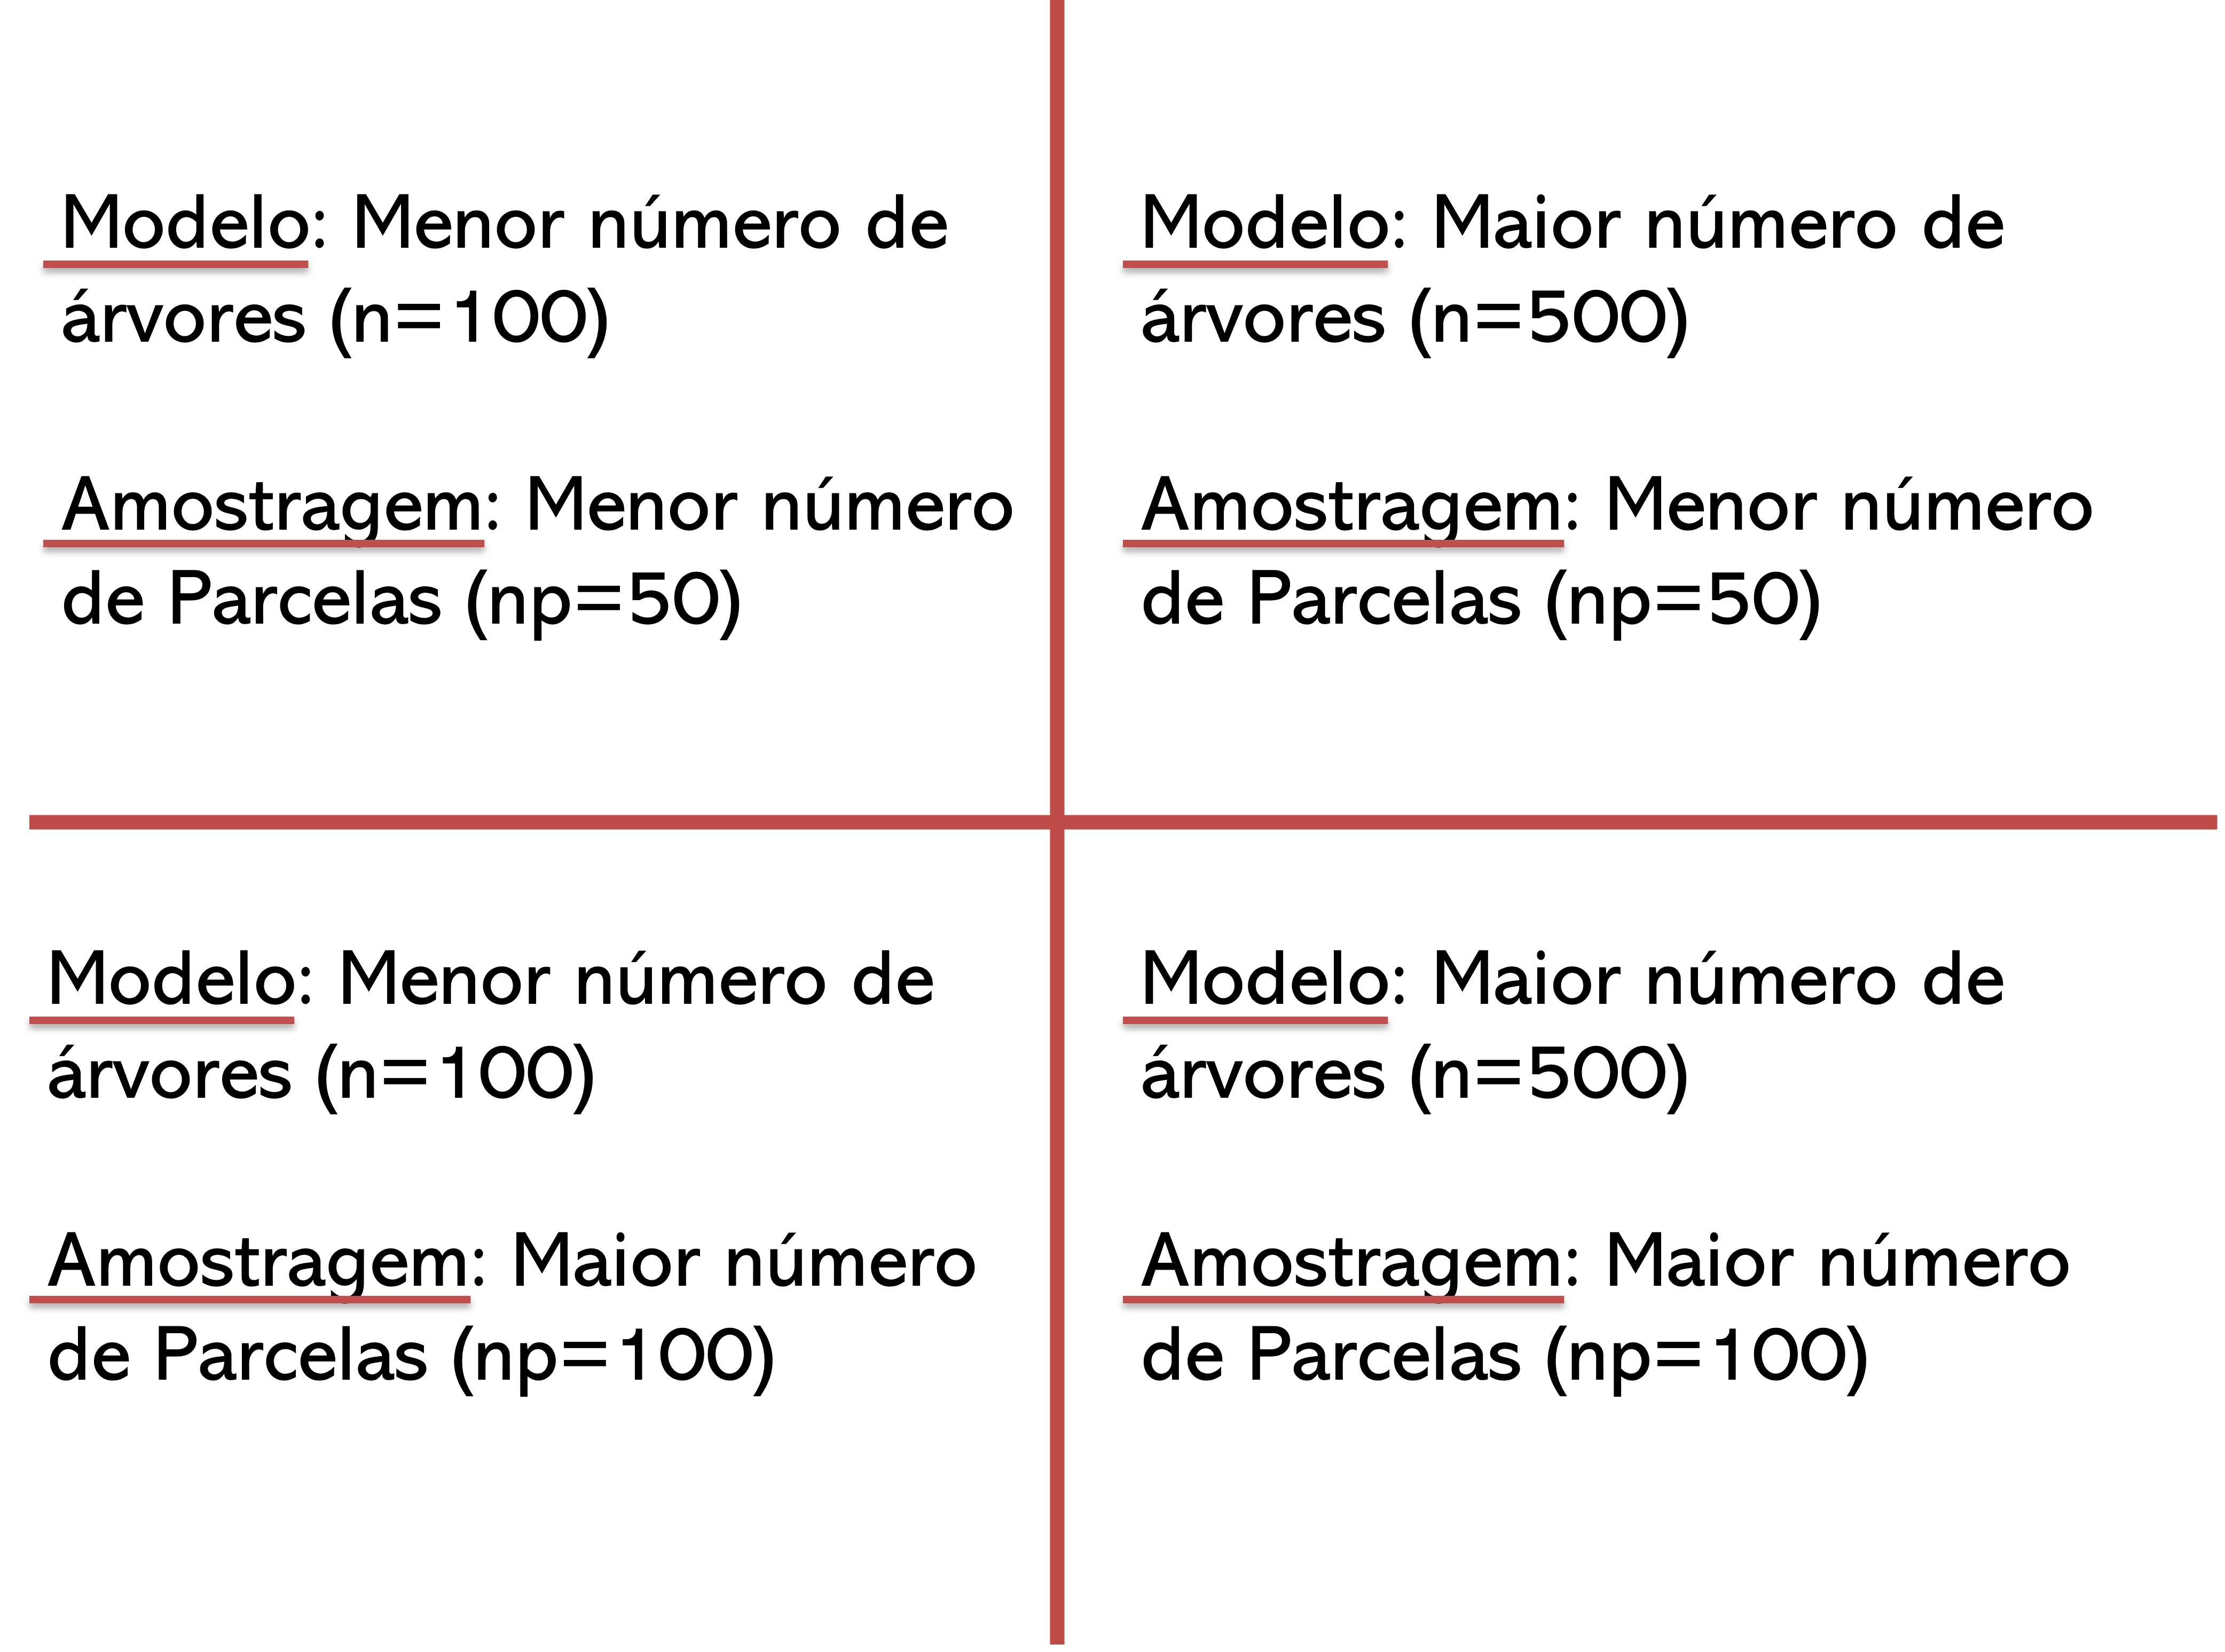
\includegraphics[width = 10cm, height = 8cm]{pic/pratico.jpg}
        \end{figure}
\end{frame}

\section{Results}
\begin{frame}{Results}
\begin{table}[]
\caption{Uncertainty results.}
\begin{tabular}{lllll}
\hline
                & Model & Sampling & CI       & Mean     \\
                \hline
Uncertainty 1   & 8.45  & 91.55    & 15068.69 & 246436.7 \\
Uncertainty 2   & 2.85  & 97.15    & 13933.46 & 238360.3 \\
Uncertainty 3   & 15.56 & 84.43    & 9528.58  & 231240.5 \\
Uncertainty   4 & 5.01  & 94.99    & 9203.42  & 223731.9\\
\hline
\end{tabular}
\end{table}
\end{frame}



\begin{frame}{Results}
The confidence interval around the mean.
\begin{figure}
        \centering
        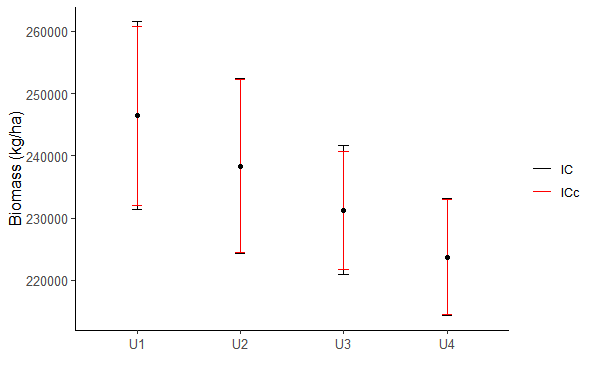
\includegraphics[width = 10cm, height = 6cm]{pic/resultado1.png}
        \end{figure}
\end{frame}

\begin{frame}{Resultados}
Contribution of each source - modelling and sampling - to the total uncertainty.
\begin{figure}
        \centering
        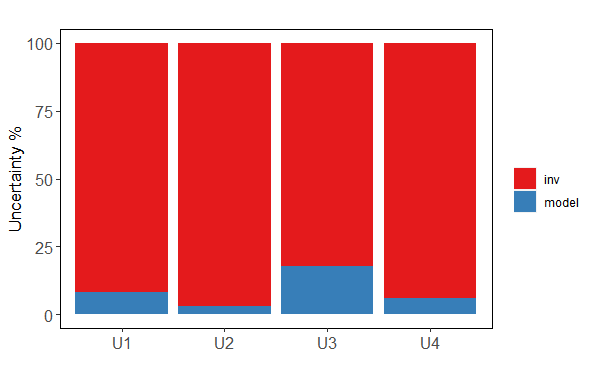
\includegraphics[width = 10cm, height = 6cm]{pic/Resultado2.png}
        \end{figure}
\end{frame}

\section{Q\&A}
\begin{frame}{Q\&A}
\begin{itemize}
    \item Questions and discussions on the topics presented.
\end{itemize}
\begin{figure}
        \centering
        
\includegraphics[width = 10cm, height = 6cm]{pic/q&a.jpg}
        \end{figure}
\end{frame}

\begin{frame}
\centering
\resizebox{!}{1cm}{Thank you!}
\resizebox{!}{1cm}{Obrigada!}
\resizebox{!}{1cm}{Gracias!}
\begin{figure}
        \centering
        
\includegraphics[width = 7cm, height = 3cm]{polyu.png}
\end{figure}
\end{frame}



\end{document}
